%%%%%%%%%%%%%%%%%%%%%%%%%%%%%%%%%%%%%%%%%%%%%%%%
% This is the official Latex template prepared by the
% Vanderbilt University Graduate School for submission of dissertations.
% It is based on a template originally prepared by
% Eli Hooten and updated by Haley Adams.

% Using the template is no guarantee that you pass format review with your
% first submission, but it should save you significant amount of time.

% This template is correct as of March 2021.
%%%%%%%%%%%%%%%%%%%%%%%%%%%%%%%%%%%%%%%%%%%%%%%%

\listfiles
\documentclass[10pt]{report}  %%% Changed from 12pt.

%%% From template

\usepackage[intoc]{nomencl}

\textwidth=6in \oddsidemargin=0.5in \topmargin=-0.5in
\textheight=9in  % 9in must include page numbers
\textfloatsep = 0.4in \addtocontents{toc}{\vspace{0.4in} \hfill
Page\endgraf} \addtocontents{lof}{\vspace{0.2in} \hspace{0.13in} \
Figure\hfill Page\endgraf} \addtocontents{lot}{\vspace{0.2in}
\hspace{0.13in} \ Table\hfill Page\endgraf}

% We've already imported some of the most commonly used packages for inserting
% formulas, images, tables, and references.
% If you need more, you can find a list of Latex packages
% here: https://www.ctan.org/pkg/

%\usepackage{textcomp}
\usepackage{array}
\usepackage{listings}
\usepackage{setspace}
%\usepackage{mathptmx}
\usepackage[table, svgnames]{xcolor}
\usepackage{colortbl}
\usepackage{graphicx}
\usepackage{amssymb,amsmath}
\usepackage{subfig}
\usepackage{epsfig}
\usepackage{times}
\usepackage{float}
\usepackage{rotating}
\usepackage{makeidx}
\usepackage{url}
\usepackage{multirow}
\usepackage{booktabs}
\usepackage{tabularx}

\usepackage[subfigure,titles]{tocloft}
\usepackage{acronym}
\usepackage{datetime}

%%another algorithm package
\usepackage{algorithm}
\usepackage{algorithmic}

\makenomenclature

\graphicspath{{Figures/}}
\DeclareGraphicsExtensions{.pdf,.jpeg,.png,.PNG,.eps,.tiff}

\urlstyle{same}

\usepackage{makecell}
\usepackage[nottoc]{tocbibind}
\usepackage{titletoc}
\usepackage{sfchap}
\usepackage{sfsection}
\usepackage[authoryear]{natbib}
%\usepackage{apacite}
\usepackage{appendix}
%\usepackage{tocbibind}

%\usepackage[nottoc]{tocbibind}
\setcounter{secnumdepth}{7}
\setcounter{tocdepth}{7}

\usepackage{tikz}
\usetikzlibrary{shapes.geometric,arrows}
\tikzstyle{box} = [ rectangle, rounded corners, minimum width = 10em, %
                    minimum height = 3em,text centered, draw = black, %
                    fill = blue!20 ]
\tikzstyle{arrow} = [thick,->,>=stealth]

\usepackage{hyperref}
\hypersetup{
  pdftitle={A LaTeX Format for Theses and Dissertations},
  pdfauthor={Eli Hooten},
  bookmarksnumbered, %Determined if chapter numbers are included in the bookmark list
  pdfstartview={FitH},
  pdfborder={0 0 0},
  plainpages=false
}
\usepackage[all]{hypcap}

% Prevent double spaced equations
\newenvironment{tightequation}{\singlespace\begin{equation}}{\end{equation}}

% Extra junk to pretty up the table of contents
\setlength{\cftsecnumwidth}{2.8em}
\setlength{\cftsubsecnumwidth}{3.7em}
\setlength{\cftsubsubsecnumwidth}{4.6em}
\setlength{\cftparanumwidth}{5.5em}
\setlength{\cftsubparanumwidth}{6.5em}
\setlength{\cfttabnumwidth}{3.5em}
\setlength{\cftfignumwidth}{3.5em}

% Prevents the splitting of long footnotes across multiple pages.
% Use with caution.
\interfootnotelinepenalty=10000

\usepackage[T1]{fontenc}
\usepackage{lmodern}
\newcommand\Fontvi{\fontsize{9}{9.2}\selectfont}

%% From Accretion Shock paper
%------------------------------------------------------------------------------%
% Packages

%\usepackage{amsmath}
\usepackage{aasmacros} % For journal symbols
\usepackage{duckuments} % For the ducks
\usepackage{soul} % To strike out multiple lines

%% From methods paper
% Define \bigtimes, taken from
% https://tex.stackexchange.com/questions/202527/writing-x-as-a-symbol-with-limits
\DeclareFontFamily{U}{mathx}{\hyphenchar\font45}
\DeclareFontShape{U}{mathx}{m}{n}{
      <5> <6> <7> <8> <9> <10>
      <10.95> <12> <14.4> <17.28> <20.74> <24.88>
      mathx10
      }{}
\DeclareSymbolFont{mathx}{U}{mathx}{m}{n}
\DeclareFontSubstitution{U}{mathx}{m}{n}
\DeclareMathSymbol{\bigtimes}{1}{mathx}{"91}

%%% From template

\renewcommand{\nomname}{LIST OF ABBREVIATIONS}

% Stats table label
\newcommand{\statslabel}[2]{\multirowcell{#1}[-1.6mm][c]{#2}}

% Below heading rule.
\newcommand{\otoprule}{\midrule[\heavyrulewidth]}

\renewcommand{\contentsname}{TABLE OF CONTENTS}
\renewcommand{\listfigurename}{LIST OF FIGURES}
\renewcommand{\listtablename}{LIST OF TABLES}
\renewcommand{\bibname}{ \texorpdfstring{{References\vspace{10mm}}}{References}   }
%
\renewcommand{\chaptermark}[1]{%
  \markboth{\MakeUppercase{%
      \chaptername}\ \thechapter.%
    \ #1}{}}

%%% From Accretion Shock Paper
%------------------------------------------------------------------------------%
% Results
\newcommand{\PeriodRatioGRoverNRxiA}{1.19}
\newcommand{\PeriodRatioGRoverNRxiB}{1.15}
\newcommand{\PeriodRatioGRoverNRxiC}{1.22}
\newcommand{\PeriodRatioGRoverNRxiD}{1.29}
\newcommand{\GrowthRateRatioGRoverNRxiA}{0.96}
\newcommand{\GrowthRateRatioGRoverNRxiB}{0.79}
\newcommand{\GrowthRateRatioGRoverNRxiC}{0.68}
\newcommand{\GrowthRateRatioGRoverNRxiD}{0.47}
\newcommand{\RelDiffAAxiA}{0.29}
\newcommand{\RelDiffAAxiB}{0.14}
\newcommand{\RelDiffAAxiC}{0.05}
\newcommand{\RelDiffAAxiD}{0.17}
\newcommand{\RelDiffACxiA}{0.21}
\newcommand{\RelDiffACxiB}{0.22}
\newcommand{\RelDiffACxiC}{0.10}
\newcommand{\RelDiffACxiD}{0.12}

% Production Codes
\newcommand{\flashx}{\textsc{\texttt{Flash-X}}}
\newcommand{\cocov}{\textsc{CoCoNuT-VERTEX}}
\newcommand{\zelmani}{\textsc{\texttt{Zelmani}}}
\newcommand{\fornax}{\textsc{Fornax}}
\newcommand{\nadafld}{NADA-FLD}
\newcommand{\chimera}{\textsc{Chimera}}
\newcommand{\gmunu}{\texttt{Gmunu}}
\newcommand{\tenet}{\textsc{tenet}}
\newcommand{\spectre}{SpECTRE}

% Math
\newcommand{\p}{\partial}
\newcommand{\pd}[2]{\frac{\partial#1}{\partial#2}}
\newcommand{\td}[2]{\frac{d#1}{d#2}}
\newcommand{\T}{^{\top}}
\newcommand{\mystackrel}[2]{\stackrel{\scriptstyle#1}{\scriptstyle#2}}

% Aliases
\newcommand{\arl}{\mathrm{areal}}
\newcommand{\iso}{\mathrm{iso}}
\newcommand{\wt}{\widetilde}
\newcommand{\etac}{\eta_{\mathrm{c}}}
\newcommand{\rpns}{R_{\textsc{pns}}}
\newcommand{\rsh}{R_{\mathrm{sh}}}
\newcommand{\rac}{R_{\mathrm{ac}}}
\newcommand{\rsc}{R_{\mathrm{Sc}}}
\newcommand{\gammabar}{\overline{\gamma}}
\newcommand{\myeqref}[1]{Eq.~(\ref{#1})}
\newcommand{\thornado}{\texttt{thornado}}
\newcommand{\amrex}{\texttt{AMReX}}
\newcommand{\eos}{EoS}
\newcommand{\cfc}{CFC}
\newcommand{\degrees}{^{\circ{}}}
\newcommand{\mdot}{\dot{M}}
\newcommand{\gr}{\textsc{gr}}
\newcommand{\nr}{\textsc{nr}}
\newcommand{\tauad}{\tau_{\mathrm{ad}}}
\newcommand{\tauac}{\tau_{\mathrm{ac}}}
\newcommand{\tac}{T_{\mathrm{ac}}}
\newcommand{\taa}{T_{\mathrm{aa}}}
\newcommand{\mpns}{M_{\textsc{pns}}}
\newcommand{\bs}[1]{\boldsymbol{#1}}
\newcommand{\mc}{\mathcal}
\newcommand{\bb}{\mathbb}
\newcommand{\appref}[1]{Appendix~\ref{#1}}
\newcommand{\figref}[1]{Figure~\ref{#1}}
\newcommand{\tabref}[1]{Table~\ref{#1}}
\newcommand{\secref}[1]{Section~\ref{#1}}
\renewcommand{\th}{-th}
\newcommand{\nModels}{\repl{5}{7}}
\newcommand{\scipy}{\texttt{scipy}}
\newcommand{\curvefit}{\texttt{curve\_fit}}

\newcommand{\repl}[2]{{}\textbf{#2}}
\newcommand{\Dbar}{\bar{D}}
\newcommand{\Deltabar}{\bar{\Delta}}
\newcommand{\weaklib}{\texttt{weaklib}}
\newcommand{\poseidon}{\texttt{Poseidon}}
\newcommand{\xcfc}{xCFC}
\newcommand{\bc}[1]{\bs{\mc{#1}}}
\newcommand{\wh}{\widehat}
\newcommand{\myol}{\overline}
\newcommand{\bj}{\left(\bs{j}\right)}
\newcommand{\Vshear}{V_{\mathrm{shear}}}
\newcommand{\myne}{n_{\mathrm{e}}}
\newcommand{\myNe}{N_{\mathrm{e}}}
\newcommand{\NK}{N_{K}}
\newcommand{\NSSPRK}{N_{\textsc{ssprk}}}

% Units
\newcommand{\msun}{M_{\odot}}
\newcommand{\erg}{\mathrm{erg}}
\newcommand{\g}{\mathrm{g}}
\newcommand{\cm}{\mathrm{cm}}
\newcommand{\km}{\mathrm{km}}
\newcommand{\s}{\mathrm{s}}
\newcommand{\kb}{k_{\textsc{B}}}
\newcommand{\K}{\mathrm{K}}
\newcommand{\J}{\mathrm{J}}
\newcommand{\ms}{\mathrm{ms}}
\newcommand{\Hz}{\mathrm{Hz}}
\newcommand{\rad}{\mathrm{rad}}

% Colors
\newcommand{\red}[1]{\textcolor{red}{#1}}
\newcommand{\blue}[1]{\textcolor{blue}{#1}}
\newcommand{\magenta}[1]{\textcolor{magenta}{#1}}
\newcommand{\cyan}[1]{\textcolor{cyan}{#1}}
\newcommand{\teal}[1]{\textcolor{teal}{#1}}
\newcommand{\orange}[1]{\textcolor{orange}{#1}}
\newcommand{\green}[1]{\textcolor{green}{#1}}

% Editing
\newcommand{\citeme}{\red{(CITE ME)}}
\newcommand{\sd}[1]{\texttt{\red{(SD: #1)}}}
\newcommand{\ee}[1]{\texttt{\blue{(EE: #1)}}}
\newcommand{\khb}[1]{\texttt{\orange{(KHB: #1)}}}
\newcommand{\KHB}[1]{\texttt{\orange{(KHB: #1)}}}
\newcommand{\am}[1]{\texttt{\cyan{(AM: #1)}}}
\newcommand{\bg}[1]{\texttt{\teal{(BG #1)}}}
\newcommand{\su}[1]{\texttt{\green{(SU #1)}}}


\begin{document}

%%%%%%%%%%%%%%%%%%%%%%%%%%%%%%%%%%%%%%%%%%%%%%%%%%%%%%%%%%%%%%%%%%%%%%%%%%%%%%%%
%% Prevent the warning: pdfTeX warning (ext4):
% destination with the same identifier (name{page.1}) has been already used,
% duplicate ignored.
% This setting will make a difference to the output because the page number
% is suppressed for the title page
\pagenumbering{alph}

\begin{titlepage}
\thispagestyle{empty}\enlargethispage{\the\footskip}%
\begin{center}
\hspace{1em}\vspace{6em} \\ % add space before content
{\setstretch{1.66}
\MakeUppercase{\thornado-Hydro, xCFC: A Discontinuous Galerkin Hydrodynamics %
Solver for General Relativistic %
Core-Collapse Supernova Simulations}\par }%
\vskip.4in
By
\vskip .4in
{Samuel John Dunham}
\vskip .4in
\begin{doublespace}
Dissertation\\
Submitted to the Faculty of the \\
Graduate School of Vanderbilt University \\
in partial fulfillment of the requirements \\
for the degree of \\ [.2in]
\end{doublespace}

DOCTOR OF PHILOSOPHY \\[.1in]
in \\[.2in]
Astronomy \& Astrophysics \\[.2in]
May 10, 2024 \\[.2in]
% The date will reflect your proposed degree conferral date as selected
% from the Intent to Graduate form.
% This is your actual graduation date, not your thesis or defense date.

Nashville, Tennessee
\vskip .5in
\end{center}

%%%Uncomment for Signatures%%%
\noindent Approved: \hskip 2.96in Date:\\[1.2em]
\rule[-3pt]{3.5in}{.5pt} \hskip 0.1in \rule[-3pt]{2in}{.5pt} \newline
  {\Fontvi\noindent Kelly Holley-Bockelmann, Ph.D.} \\[0.1in]
\rule[-3pt]{3.5in}{.5pt} \hskip 0.1in \rule[-3pt]{2in}{.5pt} \newline
  {\Fontvi\noindent Eirik Endeve, Ph.D.} \\[0.1in]
\rule[-3pt]{3.5in}{.5pt} \hskip 0.1in \rule[-3pt]{2in}{.5pt} \newline
  {\Fontvi\noindent Anthony Mezzacappa, Ph.D.} \\[0.1in]
\rule[-3pt]{3.5in}{.5pt} \hskip 0.1in \rule[-3pt]{2in}{.5pt} \newline
  {\Fontvi\noindent William Gabella, Ph.D.} \\[0.1in]
\rule[-3pt]{3.5in}{.5pt} \hskip 0.1in \rule[-3pt]{2in}{.5pt} \newline
  {\Fontvi\noindent Sait Umar, Ph.D.}

%%%%%%Uncomment  for Approved Names%%%%%%
%\begin{center}
%  \begin{doublespace}
%  Approved:\\ [.2in]
%  Professor Kelly Holley-Bockelmann \\  [.1in]
%  Professor Eirik Endeve \\  [.1in]
%  Professor Anthony Mezzacappa \\ [.1in]
%  Professor William Gabella \\ [.1in]
%  Professor Sait Umar
%  \end{doublespace}
%\end{center}

\end{titlepage}


%%%%%%%%%%%%%%%%%%%%%%%%%%%%%%%%%%%%%%%%%%%%%%%%%%%%%%%%%%%%%%%%%%%%%%%%%%%%%%%%
\doublespacing
\pagenumbering{roman} \setcounter{page}{2}

% These 3 Chapters are optional
\singlespacing
%\chapter*{}
\hspace{1em}\vspace{18em} \\ % add space before content
\begin{center}
  Copyright {\textcopyright} 2024 Samuel John Dunham \\
  All Rights Reserved
\end{center}

%
%%%%%%%%%%%%%%%%%%%%%%%%%%%%%%%%%%%%%%%%%%%%%%%%%%%%%%%%%%%%%%%%%%%%%%%%%%%%
\chapter*{}
%\addcontentsline{toc}{chapter}{ACKNOWLEDGMENTS}
\hspace{1em} \vspace{17em} \\ % add space before content 
\begin{center}
The dedication page is optional. The Copyright page is also optional. If you do not use them, please delete them. If you have a dedication, then center it in the middle of this page. If no Copyright page, begin printing page numbers here, using lower case Roman numerals and continue consecutive Roman numeral numbering throughout the preliminary pages.
\end{center}
 

%%%%%%%%%%%%%%%%%%%%%%%%%%%%%%%%%%%%%%%%%%%%%%%%%%%%%%%%%%%%%%%%%%%%%%%%%%%%
\chapter*{ACKNOWLEDGMENTS}
%\addcontentsline{toc}{chapter}{ACKNOWLEDGMENTS}
\vspace{7mm}

\begin{doublespace}

When I began to write this section, I quickly realized that to truly
acknowledge everyone that merits acknowledgement I would have to recount
my entire life story.
This is mostly due to determinism: where I am now is a complicated function
of every decision that I, and everyone else, has made.
Since my memory isn't good enough to recall every decision, I can only do my
best to thank all of those that have contributed to this dissertation,
both tangibly and intangibly.

In roughly chronological order, I would first like to thank Mr. Kapp,
my first college-level physics teacher, who
helped to keep my physics knowledge grounded in practicality.
Secondly, I would like to thank Mr. Quail, my calculus II teacher
who really let me know that I had
a natural aptitude for math, even at the college level.
Once I graduated from Washtenaw Community College and transferred to the
University of Michigan, professor Keren Sharon put me on the research track
by asking me if I would like to work with her.
I would not have had the confidence to ask a professor such a question,
so that was a pivotal moment for my career.
She went on to be my undergraduate advisor, and could not have been more
supportive of me and my future.
When I didn't get into any graduate schools, professor Nuria Calvet went out
of her way to mention me to Keivan Stassun, a professor at Vanderbilt
who was a co-founder of the Fisk-Vanderbilt Master's-to-PhD Bridge Program.
Another pivotal moment happened when I applied and was accepted into the
bridge program, and thanks to that goes to Nuria (and a little to me,
for being so great that I was accepted).
Once there, I met Kelly Holley--Bockelmann, a professor who would become the
co-chair of both my Master's and Ph.D. dissertation committees.
Again, I could not have asked for a better or more supportive person to be
(in some sense) in charge of my future.
Kelly introduced my to professor Anthony Mezzacappa,
who would also be on both of my
committees, and professor Eirik Endeve,
who would be co-chair of both of my committees.
Yet again, I was fortunate to have great and supportive people helping me to
navigate my future.
In case it isn't well known,
it is certainly not always the case to have a committee
loaded with people who truly have your best interests in mind.

Of course, a dissertation requires much more than academic guidance.
I also thank my wife, Kate, for her unyielding support throughout this journey.
Again, it is unfortunately not the case that one's spouse is always so
supportive, and I am very lucky that Kate has been.
I also thank my parents, Sandy and Steve, for their support and encouragement.
My life, like most people's, has been a bit of an emotional rollercoaster,
and they have always been there and have been supportive of my decisions.
I also want to thank my brother, Cal, to whom I have looked up since I was
very young and continue to do so today.
I thank my grandparents, Jack and Jean, who always knew the value
of education and who helped me begin my academic journey with a college fund.
I know they would be beyond proud to see how far I've come.

In addition to academic and family support, my journey has been greatly
helped by my friends and peers.
Moving to a new state is tough, and
getting through the graduate classes was much easier because of my
bridge cohort, Dax, Antonio, and Natasha, as well as other members of the
Vanderbilt astronomy group, Savannah, John, Karl, George, Laura, and Victor.
You all helped me get through this, and I am grateful to you all.
Thanks also to my childhood friends from Michigan,
Jeff, Evan, Travis, Kris, and Scott.
You've always been there for me and always made coming home extra special.

Lastly, I thank my pets, Lily, Daisy, Bo, and Penny.
They all gave and give so much joy and fun and enrich my life tremendously.

My sincerest apologies to anyone I left out, but please know that appreciate
you.

\end{doublespace}


%%%%%%%%%%%%%%%%%%%%%%%%%%%%%%%%%%%%%%%%%%%%%%%%%%%%%%%%%%%%%%%%%%%%%%%%%%%%%%%%
\singlespacing
\tableofcontents

%%%%%%%%%%%%%%%%%%%%%%%%%%%%%%%%%%%%%%%%%%%%%%%%%%%%%%%%%%%%%%%%%%%%%%%%%%%%%%%%
\begingroup
\setlength{\parskip}{1\baselineskip}
\listoftables
\newpage
\listoffigures
\newpage
%\printnomenclature %list of abbreviations is optional
%\newpage
\endgroup

%%%%%%%%%%%%%%%%%%%%%%%%%%%%%%%%%%%%%%%%%%%%%%%%%%%%%%%%%%%%%%%%%%%%%%%%%%%%%%%%
\normalsize
\doublespacing
\pagenumbering{arabic}
\setcounter{page}{1}

\chapter{Introduction}

Core-collapse supernovae are sources of some of the most extraordinary and
exquisite objects in the Universe, ranging from the microscopic heavy elements
they synthesize to the macroscopic neutron stars/pulsars in
which they often result.
In addition, they are unique laboratories in which we can probe areas of
physics which are otherwise difficult, if not impossible, to probe with
terrestrial-based experiments; e.g. nuclear matter and neutrinos.
During a core-collapse supernova (CCSN), the progenitor releases its immense
gravitational potential energy ($\sim10^{46}$ J), of which a mere 1\% goes into
the spectacular luminous displays we observe, while the remaining 99\% goes
into the dramatic release of neutrinos and antineutrinos of all flavors.
However, the gory details of exactly how a CCSN explodes are yet to be resolved.

Due in part to the fact that supernovae can outshine their entire host galaxy,
they have been observed for centuries, with some even visible during the
daytime!
However, it wasn't until the early 20th century that anyone had any ideas about
what they were \citep{bw2017}.
By studying the spectra of supernovae (SNe) it was discovered that there were,
broadly speaking, two distinct types: those whose spectra contained hydrogen
lines, and those whose spectra did not contain hydrogen lines.
Those whose spectra did not contain hydrogen lines were labeled as Type I,
and those whose spectra did contain hydrogen lines were labeled as Type II.
As more spectra were studied, it was found that there were subclasses of these
two types.
For example, a Type IIP supernova shows a plateau in its light curve,
whereas other SNe do not.
One particular subclass of Type I SNe, Type Ia, are thought to be the result of
white dwarves accreting matter to the point at which they reach their effective
Chandrasekhar masses and undergo thermonuclear explosions.
While these types of SNe are important,
but they are not the focus of this dissertation.
The Type II SNe, along with the Types Ib and Type Ic SNe, are thought to be
{\it core-collapse supernovae}.
These result, as the name implies, from the collapse of the core of a
massive star.
This results in a tremendous explosion, expelling much of the outer-layers of
the star, while keeping many heavy nuclei bound-up in the core
of the newly formed {\it proto-neutron star} (PNS).

The light-curves of SNe vary from type to type, but they do share a general
trend: they rise to a maximum on the order of days
(the so-called {\it pre-maximum phase}) and then they drop, nearly linearly in
magnitudes (exponentially in flux), for weeks.
The period of maximum light is thought to be the moment that the shock reaches
the photosphere of the stellar envelope \citep{bw2017}.

The spectra of SNe also provide a wealth of information.
Spectra are the only means we have to ascertain the composition of a SN as a
function of physical depth within the SN.
This is because as the SN ejecta expand, the optical depth lessens,
exposing deeper layers of the star \citep{bw2017}.
This is one way in which the distributions of heavy elements by CCSNe can be
deduced.

In order to understand and appreciate the products of CCSNe we need to
understand how they operate.
The following paragraph is a paraphrase from the review article \citet{m2005}.
The basic picture is that when a massive star
(ZAMS mass $M\gtrsim8\,M_{\odot}$) runs out of fuel, gravity overcomes pressure
and the star begins to collapse.
The collapse of the central iron-core separates into two pieces: a subsonically
collapsing ``inner-core" and a supersonically collapsing ``outer-core".
The collapse of the inner-core is eventually stopped because the nuclei are
forced into such close proximity with each other that they undergo a
phase transition from individual nuclei to bulk nuclear matter
(the creation of a PNS),
causing the pressure to increase drastically as a result of the repulsive
nature of the strong force.
At this point the core is supported by a combination of the strong force and
neutron degeneracy pressure.
The still infalling outer-core collides suddenly with the newly formed PNS,
generating a strong shock wave that propagates outward, ultimately driving
the explosion.
It is intuitive that the shock wave simply propagates outward, disrupting
the star.
Unfortunately, as often happens, reality is not so simple.

As the shock propagates, it loses energy to the newly-created and liberated
(anti)neutrinos as well as to the dissociation of the
infalling material through which it passes,
so much so that the shock stalls around 200 km from the center
(e.g., see \citet{hm1981}).
It is clear that the shock is revived, because if it weren't then matter
would continue to accrete onto the star, eventually making the core massive
enough to overcome the strong force and the neutron degeneracy pressure
and cause the PNS to collapse
to a black hole \citep{bw1985}.
(This does happen under certain conditions, but they are not discussed here.)

\sd{LEFT OFF HERE}

It was discovered numerically that while the shock is stable to
perturbations in 1D models, it is unstable to non-radial perturbations
in 2D models \citep{bmd2003}.
This purely hydrodynamical instability has since become known as the
standing accretion shock instability (SASI), and it very likely plays an
important role in the explosion mechanism for more massive progenitors.
This discovery also strongly implies that supernova explosions are
inherently multi-dimensional.

One effect of the SASI is turbulence generated below the shock,
which can increase the amount of time that a fluid particle spends
in the ``gain region", a region below the shock in which there is a
net heating due to neutrinos \citep{co2015}.
Since the fluid spends more time in this region it can be heated more than if
SASI-driven turbulence were absent.
This extra heating can help revive the shock.
Multi-dimensional models are necessary for several reasons,
one of which is that turbulence is non-existent in 1D, and in 2D it
exhibits an inverse-cascade, where energy is artificially transmitted
from small-scale eddies to large-scale eddies \citep{yem2017}.
Therefore, to truly study turbulence in CCSNe we need 3D simulations,
with no assumptions of symmetry.

Although fusion stops once it reaches iron, CCSNe produce elements of much
higher atomic mass number, $A$.
In fact, CCSNe are responsible for most of the elements in the Universe with
$16\lesssim A\lesssim90$ \citep{bw2017}.
Two products in particular, $^{56}$Ni and $^{57}$Ni, are critical for SN light
curves (their half-lives correlate well with the decline of the light curve),
and the amounts of these elements depend on the explosion mechanism.
The explosion energy is sufficient to expel the matter away from the star
and throughout the galaxy, enriching it with heavy elements otherwise that have
no earthly business in the ISM\footnote{Or a Maine hayfield...}.
The distribution of metals in galaxies has implications for galactic
evolution, so an understanding of how the heavy elements are distributed,
and especially how much of each element is distributed,
is crucial for galaxy evolution models.

One of the elements produced and distributed is carbon,
the element on which life as we know it is based, so there is additionally
a metaphysical reason to understand CCSNe:
It is to them that we literally owe our entire existence!

The most obvious products of CCSNe are the copious amount of photons
released in the explosion process.
However, preceding the fireworks is something arguably much more interesting
and magnificent---the gravitational waves emitted from the asymmetry of the
mass-energy distribution.
These waves will be more like bursts, lasting less than one second,
but will be in the LIGO band and should be detectable by aLIGO
out to several kpc \citep{aaa2016}.
From full simulations of CCSNe we obtain the components of the stress-energy
tensor, from which we can compute the mass-quadrupole moment,
which can tell us the waveforms of the gravitational waves emitted.
The inclusion of GR hydrodynamics will produce waveforms that are more
faithful to nature than those that currently exist.

Another product of CCSNe is the plethora of neutrinos released.
As mentioned earlier, about 99\% of the energy in a CCSN
(amounting to approximately $0.15\,\msun\,c^{2}$) is carried away by neutrinos.
These weakly interacting particles are some of the most elusive particles known.
Their practically infinitesimal cross-section makes them extremely difficult
to detect.
A CCSN is one of the few phenomena that produces a sufficient amount of
neutrinos that we can detect them on Earth.

Modeling CCSNe is no trivial task.
There are, broadly speaking, three branches of physics at play:
gravity, neutrino transport, and hydrodynamics.
As mentioned earlier, the SASI is a purely hydrodynamic instability and so
I will focus on the hydrodynamics component.
One aspect of hydrodynamics that makes numerical methods challenging is the
possibility of discontinuities in the flow---shocks.
These pose a problem because the equations that govern hydrodynamics are
partial differential equations, and therefore are not well-defined in the
vicinity of shocks.
There has been much work in this field, and we are able to take advantage of
some of this work.
By casting the hydrodynamics equations in conservative form we can identify
the equations as a hyperbolic conservation law, and can make use of the
extensive literature on this subject (see, e.g., \citet{l2002}).

We are developing a new code to simulate CCSNe,
the \textbf{t}oolkit for \textbf{h}igh-\textbf{or}der
\textbf{n}eutrino-r\textbf{ad}iation hydr\textbf{o}dynamics, \thornado.
For the hydrodynamics we employ a discontinuous Galerkin spatial discretization
\citep{cs1998} and an explicit strong-stability-preserving Runge-Kutta temporal
discretization.
The discontinuous Galerkin (DG) method is ideal for hydrodynamics because of,
among other aspects, its locality (communication with nearest neighbors only,
independent of the desired order of accuracy),
which makes it adept at handling shocks as well as parallelizability.
The code has been tested against several challenging test-problems,
including problems with smooth solutions, such as a Kelvin-Helmholtz
instability problem, and problems with strong shocks in multiple dimensions,
such as 2D Riemann problems.
The SASI problem is physically-motivated but can be treated with
pure hydrodynamics, i.e. not making use of the gravity solver or the
neutrino transport solver,
making it an excellent test problem to probe the robustness of \thornado.
The SASI problem has been tested with \thornado\ in two spatial dimensions
with non-relativistic hydrodynamics.
This work will extend that to three spatial dimensions and GR hydrodynamics.
An additional complexity that arises with numerically modeling hydrodynamics
is that the time-step is often very short as a result of the CFL condition.
In order to complete a simulation on a reasonable timescale a
hydrodynamics code benefits greatly from parallelizability.

We have coupled \thornado\ to
\amrex\footnote{https://amrex-codes.github.io/amrex/},
a block-structured AMR code being developed primarily out of
Lawrence-Berkeley National Laboratory.
In addition to AMR, \amrex\ has parallel capabilities, and it is these
capabilities of which we make use in this work.
The non-relativistic hydrodynamics component of \thornado\ has been
incorporated with \amrex, and can successfully run within the
\amrex\ framework and benefit from the parallel capabilities.
This will serve as a guide for the implementation of the
relativistic hydrodynamics as well as, eventually, the neutrino transport.
\thornado\ can not yet interface with the AMR features of \amrex.
That will be future work.

%------------------------------------------------------------------------------%

\chapter{Accretion Shock Paper}
\label{ch.sasi}

This chapter is adapted from
``A Parametric Study of the SASI Comparing General Relativistic
and Non-Relativistic Treatments" in the Astrophysical Journal and has been
reproduced with the permission of the publisher and my co-authors
Eirik Endeve, Anthony Mezzacappa, John M. Blondin, Jesse Buffaloe, and Kelly
Holley-Bockelmann.

%------------------------------------------------------------------------------%
\section{Abstract}
We present numerical results from a parameter study of the standing accretion
shock instability (SASI), investigating the impact of general relativity (GR)
on the dynamics. Using GR hydrodynamics with GR gravity,
and non-relativistic (NR) hydrodynamics with Newtonian gravity,
in an idealized model setting, we vary the initial radius of the shock and,
by varying its mass and radius in concert, the proto-neutron star (PNS)
compactness.
We investigate four compactnesses expected in a post-bounce
core-collapse supernova (CCSN).
We find that GR leads to a longer SASI oscillation period,
with ratios between the GR and NR cases as large as \PeriodRatioGRoverNRxiD{}
for the highest-compactness suite.
We also find that GR leads to a slower SASI growth rate,
with ratios between the GR and NR cases as low as \GrowthRateRatioGRoverNRxiD{}
for the highest-compactness suite. We discuss implications of our results for
CCSN simulations.

%------------------------------------------------------------------------------%
\section{Introduction}

Since the discovery of the standing accretion shock instability
\citep[SASI;][]{bmd2003}, which many two- and three-dimensional simulations
performed to date demonstrate becomes manifest during a
core-collapse supernova (CCSN) in the post-shock accretion flow
onto the proto-neutron star (PNS),
groups have made efforts to understand its physical origin
and its effects on the supernova itself.
The SASI is characterized in two dimensions (2D) by a large-scale
``sloshing" of the shocked fluid,
and in three dimensions (3D) by additional spiral modes \citep{bm2007}.
It is now generally accepted that turbulent neutrino-driven convection
plays a major role in re-energizing the stalled shock
\citep[e.g., see][]{%
bdm2012,
hmw2013,
mdb2013,
co2015,
mjm2015,
lbh2015,
aor2015,
rco2015,
mjm2015,
mjb2015,
roh2016,
mmh2017,
sjm2018,
rao2018,
oc2018b,
vbr2019,
mth2019,
brv2019,
ytk2019,
pm2020,
sjk2020,
mv2020,
vcb2022,
ntk2022,
mat2022%
}.
The same simulations that led to the above conclusion also generally exhibit
the SASI, with outcomes ranging from convection-dominated flows to
SASI-dominated flows, and flows where neither dominates.
Strong SASI activity and, in some cases, SASI-aided explosions have been
reported in, for example, the three-dimensional simulations of
\cite{sjm2018}, \cite{oc2018b}, and \cite{mat2022}.
A more precise determination of the relative role played by these two
instabilities in the explosion mechanism, on a case-by-case basis
\citep[i.e., for different progenitor characteristics; e.g., see][]{%
sjf2008,
hmm2012,
hmw2013,
co2014,
fmf2014,
mjb2015,
aor2015,
f2015%
}, will require advances in current three-dimensional models to include full
general relativity,
rotation, magnetic fields, and the requisite neutrino interaction physics
with realistic spectral neutrino kinetics, all at high spatial resolution.
It is also important to note that, while
convection-dominated and SASI-dominated scenarios may lie at the extremes of
what is possible, it is not necessary for one or the other instability to be
dominant to play an important role -- specifically, for the more complex cases
where neither dominates,
it would be very difficult
to determine precisely the relative
contribution from these two instabilities.

Several studies have concluded that the SASI is an
{\sl  advective-acoustic} instability, in which
vortical waves generated at the shock advect to the surface of the PNS,
which in turn generate acoustic waves that propagate back to the
shock and further perturb it
\citep{fsj2006,fgs2007,yy2007,l2007,l2008,f2009,gf2012}.
This perturbation generates more, stronger, vortical waves,
which advect to
the PNS surface, thus creating a feedback loop that drives the instability.
An alternative explanation for the SASI is the
{\sl purely acoustic} mechanism, in which
acoustic perturbations just below the shock travel around
the post-shock region and constructively interfere with each other,
generating stronger acoustic perturbations
and thereby feeding the instability
\citep{bm2006}.
A recent study \citep{wft2023} suggests that the acoustic mechanism may play
a particularly important role in the SASI when rotation is included,
implying that the origins of the SASI excitation may depend on conditions
between the shock and the PNS.

Other numerical studies focus on particular aspects of this instability,
such as the hydrodynamics of the SASI
\citep{oky2006,sff2009,iny2014},
spiral modes
\citep{bs2007,iko2008,f2010},
the spin-up of the possible remnant pulsar
\citep{bm2007},
the effect of nuclear dissociation
\citep{ft2009},
saturation of the instability
\citep{gsf2010},
the generation and amplification of magnetic fields
\citep{ecb2010,ecb2012},
the relative importance of the SASI and convection in CCSNe
\citep{cb2015},
the generation of, and impact on, gravitational waves by the SASI
\citep{%
koy2007,
kio2009,
kkt2016,
a2017,
kkt2017,
amm2017,
oc2018b,
hkk2018,
amj2019,
mml2020,
mml2023,
dad2023},
and the effects of rotation
\citep{yy2005,yf2008,wft2023,bfg2023}.
Some of these studies included sophisticated microphysics, such as
realistic equations of state (\eos s) and neutrino transport;
however, with the exception of \citet{kkt2017},
none of these studies solved the general relativistic hydrodynamics (GRHD)
equations, instead solving their non-relativistic (NRHD) counterparts,
some with an approximate relativistic gravitational potential.
It has been demonstrated that GR effects are crucial to include in CCSN
simulations \citep{bdm2001,mjm2012,lmm2012,oc2018a}, yet the SASI itself
has not been fully investigated in the GR regime.
A recent paper \citep{kc2022} does analyze steady state accretion
through a stationary shock onto compact objects in a
Schwarzchild geometry and compares with Newtonian solutions, and posits
that GR may have a non-negligible impact on the SASI.
They find that, for conditions expected in exploding CCSNe,
the freefall speed is of order $v\sim0.2\,c$
(with $c$ the speed of light), and
the differences between the GR and NR solutions are of order 10\%.
For conditions expected in failed CCSNe (i.e., supernovae where the
shock is not revived, in which case the freefall speed can be
$v\sim0.66\,c$), the differences can be larger.

The timescales that likely influence the SASI depend on signal-speeds
associated with advective and acoustic modes in the region
between the shock and the PNS surface
\citep{bm2006,fgs2007,m2020}.
Motivated in part by \citet{dem2020} and \citet{kc2022},
we expect SASI simulations to behave differently depending
on whether or not the treatment of the hydrodynamics and gravity
are general relativistic.
Indeed, \citet{dem2020} presented GR steady-state solutions and
presented preliminary results from GR SASI simulations,
but did not compare results from NR and GR simulations.
Specifically, we expect both advective and acoustic modes to be
influenced by the different post-shock structure in the GR case
relative to the NR case.

This leads to our main science question:
\emph{How does a general relativistic treatment of hydrodynamics and gravity
affect the oscillation period and growth rate
of the SASI?}
To begin to address this, we
present the first comparison of the SASI in both a non-relativistic
and a general relativistic framework, using an idealized model
with four compactnesses, meant to span the range of conditions
expected in CCSN simulations.
We focus our attention on the linear regime and characterize the SASI by its
growth rate and oscillation period, as was done in \citet{bm2006}.
To capture both the linear regime of the SASI and its transition to the
nonlinear regime,
we perform our assessment via seven axisymmetric numerical
simulations using GRHD and GR gravity, with the PNS represented by a point mass
and gravity encoded in a Schwarzchild spacetime metric.
To better assess the impact of GR, we also perform simulations
using the same parameter sets but
with NRHD and Newtonian gravity, again with the PNS represented by a point
mass, but in this case gravity is encoded in the Newtonian potential.
We will often use ``NR" to refer to the case of Newtonian gravity
and NRHD.

We use a system of units in which $c=G=1$ and also make use of the Einstein
summation convention, with Greek indices running from 0 to 3 and Latin indices
running from 1 to 3.

%------------------------------------------------------------------------------%
\section{Physical Model}

\subsection{Relativistic Gravity: Conformally-Flat Condition}

We use the 3+1 decomposition of spacetime
\citep[see, e.g.,][for details]{bfi1997,g2012,rz2013},
which, in the coordinate system
$x=\left(t,x^{i}\right)$,
introduces four degrees of freedom:
the lapse function, $\alpha\left(x\right)$,
and the three components of the shift vector,
$\beta^{i}\left(x\right)$.
We further specialize to the conformally-flat condition
\citep[\cfc{},][]{wmm1996},
effectively neglecting the impact of gravitational waves on
the dynamics.
This is a valid approximation when the CCSN progenitor is non-rotating
\citep{dnf2005}, as is the case for our simulations.
The \cfc{} forces the components of the
spatial three-metric, $\gamma_{ij}\left(x\right)$,
to take the form
\begin{equation}
  \gamma_{ij}
  =\psi^{4}\,\gammabar_{ij},
  \label{eq.AP.gammaij}
\end{equation}
where $\psi\left(x\right)$ is the conformal factor
and the $\gammabar_{ij}$ are the components of a time-independent,
flat-space metric.
We choose an isotropic spherical-polar coordinate system,
as it is appropriate to our problem and is consistent with the \cfc;
the flat-space metric is
\begin{equation}
  \gammabar_{ij}\left(r,\theta\right)
  :=\mathrm{diag}\left(1,r^{2},r^{2}\,\sin^{2}\theta\right),
  \label{eq.AP.gammabarij}
\end{equation}
and the lapse function, conformal factor, and shift vector
take the form given in \citet{bs2010},
\begin{alignat}{2}
  \alpha   \left(t,r,\theta,\varphi\right)&=\alpha   \left(r\right)
    &&:=\frac{1-\rsc/r}{1+\rsc/r},\\
  \psi     \left(t,r,\theta,\varphi\right)&=\psi     \left(r\right)
    &&:=1+\rsc/r,\label{eq.AP.psi}\\
  \beta^{i}\left(t,r,\theta,\varphi\right)&=\beta^{i}\left(r\right)
    &&:=0,
\end{alignat}
where $r>\rsc$ is the isotropic radial coordinate measured from the
origin and $\rsc:=M/2$ is the Schwarzchild radius in
isotropic coordinates for an object of mass $M$.
The line element under a 3+1 decomposition in
isotropic coordinates takes the form
\begin{equation}
  ds^{2}=-\alpha^{2}\,dt^{2}+\gamma_{ij}\,dx^{i}\,dx^{j}.
  \label{eq.AP.ds2}
\end{equation}
We note here that the {\sl proper} radius, $\mc{R}\left(r\right)$,
corresponding to the {\sl coordinate} radius, $r>\rsc$, is defined by
\begin{equation}
  \mc{R}\left(r\right)
  :=\int\limits_{\rsc}^{r}\sqrt{\gamma_{11}}\,
  dr'
  =r-\rsc^{2}/r+2\,\rsc\,\log\left(r/\rsc\right)\geq r,
  \label{eq.AP.properDistance}
\end{equation}
where we used Eqs. (\ref{eq.AP.gammaij}-\ref{eq.AP.gammabarij})
with $\psi$ given by \myeqref{eq.AP.psi}.
Under the \cfc{}, the square root of the determinant of the spatial
three-metric is
\begin{equation}
    \sqrt{\gamma}=\psi^{6}\,\sqrt{\gammabar}=\psi^{6}\,r^{2}\,\sin\theta.
\end{equation}

Our choice of isotropic coordinates is consistent with our implementation of general
relativistic hydrodynamics in the CFC approximation.
Our comparison of the Newtonian and general relativistic results is conducted
{\em within this gauge}.
(In practice, the hydrodynamics equations in the Newtonian limit in the isotropic gauge
are identical {\em in form} to the standard Newtonian hydrodynamics equations,
and we were able to run our NR simulations with our Newtonian hydrodynamics code.)

\subsection{Relativistic Hydrodynamics}

We solve the relativistic hydrodynamics equations
of a perfect fluid (i.e., no viscosity or heat transfer)
in the Valencia formulation
\citep{bfi1997,rz2013}, in which they take the form of a
system of hyperbolic conservation laws with sources. Under our assumption of
a stationary spacetime, the equations can be written as
\begin{equation}\label{eq.AP.cLaws}
  \p_{t}\,\bs{U}
  +\frac{1}{\sqrt{\gamma}}\,
  \p_{i}\left(\alpha\,\sqrt{\gamma}\,\bs{F}^{i}\right)=\alpha\,\bs{S},
\end{equation}
where $\bs{U}:=\bs{U}\left(t,r,\theta,\varphi\right)$
is the vector of evolved fluid fields,
\begin{equation}
  \bs{U}
  =\begin{pmatrix}
  D\\
  S_{j}\\
  \tau
  \end{pmatrix}
  =\begin{pmatrix}
  \rho\,W\\
  \rho\,h\,W^{2}\,v_{j}\\
  \rho\,h\,W^{2}-p-\rho\,W
  \end{pmatrix},
\end{equation}
$\bs{F}^{i}:=\bs{F}^{i}\left(\bs{U}\right)$ is the vector of fluxes of those
fields in the $i$\th{} spatial dimension,
\begin{equation}
  \bs{F}^{i}
  =\begin{pmatrix}
  D\,v^{i}\\
  P^{i}_{~j}\\
  S^{i}-D\,v^{i}
  \end{pmatrix},
\end{equation}
and $\bs{S}:=\bs{S}\left(\bs{U}\right)$ is the vector of sources,
\begin{equation}
  \bs{S}
  =\begin{pmatrix}
  0\\
  \frac{1}{2}\,P^{ik}\,\p_{j}\,\gamma_{ik}
  -\alpha^{-1}\left(\tau+D\right)\,\p_{j}\,\alpha\\
  -\alpha^{-1}S^{j}\,\p_{j}\,\alpha
  \end{pmatrix},
\end{equation}
where $D$ is the conserved rest-mass density,
$S_{j}$ is the component
of the Eulerian momentum density in the $j$\th{} spatial dimension,
and $\tau:=E-D$, with $E$ the Eulerian energy density.
The component of the fluid three-velocity in the $j$\th{} spatial dimension
is denoted by $v^{j}$, and
$W:=\left(1-v^{i}v_{i}\right)^{-1/2}$ is the Lorentz factor
of the fluid, both as measured by an Eulerian observer.
The relativistic specific enthalpy as measured by an observer
comoving with the fluid; i.e., a comoving observer, is
$h:=1+\left(e+p\right)/\rho$, where
$\rho$ is the baryon mass density, $e$ is the internal energy density,
and $p$ is the thermal pressure, all measured by a comoving observer.
Finally, $P^{ij}:=\rho\,h\,W^{2}\,v^{i}\,v^{j}+p\,\gamma^{ij}$,
with $\gamma^{ij}$ the inverse of $\gamma_{ij}$; i.e.,
$\gamma^{ik}\gamma_{kj}=\delta^{i}_{~j}$.
See \citet{rz2013} for more details.

We close the hydrodynamics equations
with an ideal \eos,
\begin{equation}
  p\left(e\right)=\left(\Gamma-1\right)e,
  \label{eq.AP.idealEOS}
\end{equation}
where $\Gamma\in\left(1,2\right]$ is the ratio of specific heats.
For this study, we set $\Gamma=4/3$.
We further assume the \eos{} is that of a polytrope; i.e.,
\begin{equation}
  p\left(\rho\right)=K\,\rho^{\Gamma},
  \label{eq.AP.polytrope}
\end{equation}
where $K>0$ is the polytropic constant,
whose logarithm can be considered a proxy for the entropy, $S$;
i.e., $S\propto\log\left(p/\rho^{\Gamma}\right)$.
The constant $K$ takes different values on either side of a
shock, in accordance with physically admissible solutions.
\myeqref{eq.AP.polytrope} is consistent with \myeqref{eq.AP.idealEOS}
through the first law of thermodynamics for an isentropic fluid.

\subsection{Non-Relativistic Hydrodynamics}

Under the 3+1 formalism of GR and the CFC,
the effect of gravity is encoded in the metric via the lapse function,
the conformal factor, and the shift vector, whereas with
Newtonian gravity,
the metric is that of flat space and the effect of gravity
is encoded in the Newtonian gravitational potential, $\Phi$,
\begin{equation}
  \Phi\left(r\right):=-\frac{M}{r}.
\end{equation}
Of course, the NRHD equations can be recovered from the GRHD equations
by taking appropriate limits; i.e.,
$v^{i}v_{i}\ll1$, $p,e\ll\rho$,
and $\Phi\ll1$, and setting $\alpha\approx\alpha_{\nr}:=1+\Phi$
and $\psi=1-\Phi/2$.

In the case of Newtonian gravity and NRHD, we solve\begin{equation}
  \p_{t}\,\bs{U}
  +\frac{1}{\sqrt{\gammabar}}\,
  \p_{i}\left(\sqrt{\gammabar}\,\bs{F}^{i}\right)=\bs{S},
  \label{eq.AP.cLawsNR}
\end{equation}
where
\begin{equation}
  \bs{U}
  =\begin{pmatrix}
  D\\
  S_{j}\\
  E
  \end{pmatrix}
  =\begin{pmatrix}
  \rho\\
  \rho\,v_{j}\\
  e+\frac{1}{2}\,\rho\,v^{i}\,v_{i}
  \end{pmatrix},
\end{equation}
\begin{equation}
  \bs{F}^{i}
  =\begin{pmatrix}
  \rho\,v^{i}\\
  P^{i}_{~j}\\
  \left(E+p\right)v^{i}
  \end{pmatrix},
\end{equation}
and
\begin{equation}
  \bs{S}
  =\begin{pmatrix}
  0\\
  \frac{1}{2}\,P^{ik}\,\p_{j}\,\gammabar_{ik}
  -\rho\,\p_{j}\,\Phi\\
  -S^{j}\,\p_{j}\,\Phi
  \end{pmatrix},
\end{equation}
where
$P^{ij}:=\rho\,v^{i}\,v^{j}+p\,\gammabar^{ij}$ and we assume $\Phi$
is due only to the point source PNS,
\begin{equation}
  \Phi\left(r\right):=\frac{-\mpns}{r}.
\end{equation}

%------------------------------------------------------------------------------%
\section{Steady-State Accretion Shocks}
\label{ss.ssas}

We take initial conditions for our simulations from steady-state
solutions to \myeqref{eq.AP.cLaws} (GR) and \myeqref{eq.AP.cLawsNR} (NR).
To determine the steady-state solutions,
we assume the fluid distribution is spherically symmetric and time-independent.
Following \citet{bmd2003},
we consider a stationary accretion shock located at $r=\rsh$
with a PNS mass $\mpns$, PNS radius $\rpns$,
and a constant mass accretion rate
$\mdot>0$.
We assume a polytropic constant ahead of the shock, $K=2\times10^{14}\,
\left[\left(\erg\,\cm^{-3}\right)/\left(\g\,\cm^{-3}\right)^{4/3}\right]$,
chosen so that the pre-shock flow is highly supersonic
(all of our models have a pre-shock Mach number greater than 15).
Given that our steady-state solutions have constant
entropy between the PNS surface and the shock, they are convectively stable.
This enables us to isolate the SASI and study its development.

\subsection{Relativistic Steady-State Solutions}

Focusing on the equation for $D$, we find
(temporarily defining $v\equiv v^{r}$),
\begin{equation}
  \alpha\,\psi^{6}\,W \times 4\pi\,r^{2}\rho\,v=-\dot{M}.
  \label{IC.eq1}
\end{equation}
Manipulation of the equations for $D$ and $\tau$
in \myeqref{eq.AP.cLaws} yields the relativistic Bernoulli equation,
\begin{equation}
  \alpha\,h\,W=\mc{B},
  \label{IC.eq2}
\end{equation}
where $\mc{B}>0$ is the relativistic Bernoulli constant.
At spatial infinity, the fluid is assumed to be at rest and the spacetime
curvature negligible, so $\alpha_{\infty}=W_{\infty}=1$.
Further, at spatial infinity, we assume the fluid to be cold; i.e.,
$\left(e+p\right)/\rho\ll1$,
so that $h_{\infty}=1$ and $\mc{B}_{\infty}=1$.
Since $\mc{B}$ is a constant, $\mc{B}=1$ everywhere.

Given $K$, Eqs. (\ref{eq.AP.polytrope}), (\ref{IC.eq1}),
and (\ref{IC.eq2}) (with $\mc{B}=1$)
form a system of three equations in the three unknowns,
$\rho$, $v$, and $p$.
From initial guesses $v_{0}=-\sqrt{2\,\mpns/r}$,
$\rho_{0}=-\dot{M}/\left(4\pi\,r^{2}\,v_{0}\right)$, and
$p_{0}=K\,\rho_{0}^{\Gamma}$, the first two of which are obtained
from the Newtonian approximation at a distance $r>\rsh$ for
highly supersonic flow,
we define dimensionless variables
$u_{1}:=\rho/\rho_{0}$, $u_{2}:=v/v_{0}$, and $u_{3}:=p/p_{0}$.
These are substituted into the system of equations, which are then solved
with a Newton--Raphson algorithm to determine the state of the fluid everywhere
ahead of the shock.
To join the pre- and post-shock states of the fluid at $r=\rsh$,
we apply the relativistic Rankine--Hugoniot jump conditions
\citep[i.e., the Taub jump conditions,][]{t1948}
to obtain $\rho$, $v$, and $p$ just below the shock.
Once the state of the fluid just below the shock is found,
the polytropic constant for the post-shock fluid is computed
with \myeqref{eq.AP.polytrope}
and the same system of equations is solved for
the state of the fluid everywhere below the shock.

\subsection{Non-Relativistic Steady-State Solutions}

The steady-state solution method for the non-relativistic case
(taken from \citet{bmd2003}) follows a similar procedure
as the relativistic case,
except we begin from the NR equations for mass density and energy density,
\begin{align}
  \p_{t}\,\rho+\frac{1}{\sqrt{\gammabar}}\,
  \p_{i}\left(\sqrt{\gammabar}\,\rho\,v^{i}\right)
  &=0,\\
  \p_{t}\,E+\frac{1}{\sqrt{\gammabar}}\,
  \p_{i}\left[\sqrt{\gammabar}\left(E+p\right)v^{i}\right]
  &=-\rho\,v^{i}\,\p_{i}\,\Phi,
\end{align}
where $E:=e+\frac{1}{2}\,\rho\,\gammabar_{ij}\,v^{i}\,v^{j}$.
From these, and making the same assumptions as in the relativistic case,
we arrive at a system of two equations for the three unknowns,
$\rho$, $v\equiv v^{r}$, and $p$,
\begin{align}
  4\pi\,r^{2}\,\rho\,v&=-\dot{M},\label{eq.AP.MassConservationNR}\\
  \frac{1}{2}\,v^{2}+h_{\nr}+\Phi&=\mc{B}_{\nr},
  \label{eq.AP.BernoulliNR}
\end{align}
with $h_{\nr}=h-1=\left(e+p\right)/\rho$
the non-relativistic specific enthalpy and $\mc{B}_{\nr}$
the non-relativistic Bernoulli constant.
Following \citet{bmd2003}, we set $\mc{B}_{\nr}=0$.
As in the GR case, we close this system with \myeqref{eq.AP.polytrope}.

In the non-relativistic limit,
$\alpha\approx1+\Phi$ and $W\approx1+\frac{1}{2}\,v^{i}\,v_{i}$;
substituting these into \myeqref{IC.eq2} yields, to leading order,
$1+\mc{B}_{\nr}$,
in agreement with \myeqref{eq.AP.BernoulliNR}.

\subsection{Comparison of NR and GR Steady-State Solutions}

For the two lower-compactness cases (see \myeqref{eq.AP.compactness})
\citep[e.g., see][]{bmh2013,mjm2015,brv2020},
\figref{fig.compSS_loXi} shows steady-state accretion shock solutions
as functions of coordinate distance $r$.
(Note that in \figref{fig.compSS_loXi} and \figref{fig.compSS_hiXi} below,
for additional information, the steady-state solutions are plotted from the shock all
the way down to $r=3$~km.
For our numerical simulations, the inner boundary is placed at
$\rpns\in\{20,40\}$~km, which then defines the compactness of our models.)

In general, the magnitudes of the density, velocity,
and pressure just below the shock decrease as the shock radius increases
\citep[e.g., see Eqs. (1-3) in][]{bmd2003}.
From the top-right panel of \figref{fig.compSS_loXi},
it can be seen that the velocities in the GR and NR cases agree
well near the shock and deviate from each other for smaller radii,
with the velocity being smaller in the GR case than in the NR case.
The top-left and bottom-left panels show that the densities and pressures
in the GR case are larger than their NR counterparts at smaller radii.
The slope of the NR density profile
matches expectations of $\rho\left(r\right)\propto r^{-3}$ \citep{bmd2003},
but the GR density profile deviates noticeably
from this as the inner-boundary
is approached.
From the bottom-right panel, it can be seen that the lapse function
and its Newtonian approximation begin to deviate from each other
near $r=40\,\km$,
with the degree of deviation increasing
for smaller radii.
\begin{figure}[htb!]
  \centering
  \includegraphics[width=0.8\textwidth]%
  {fig.CompareNRvsGR_SS_loXi.pdf}
  \caption{
Post-shock, steady-state solutions for GR (solid) and NR (dashed)
equations as functions of coordinate distance $r\in\left[3\,\km,\rsh\right]$
for three models having the same
accretion rate of 0.3$\,\msun/\s$,
the same PNS mass of 1.4$\,\msun$, and shock radii
120 km (blue), 150 km (orange), and 175 km (green).
For this PNS mass, the Schwarzchild radius is $\sim$1 km.
Quantities defined just ahead of the shock are denoted with a subscript ``1".
The top-left panel shows the comoving baryon mass density
normalized to its value just ahead of the shock,
the top-right panel shows the radial component of the fluid three-velocity
normalized to its value just ahead of the shock,
the bottom-left panel shows the comoving pressure
normalized to the Newtonian ram pressure just ahead of the shock,
$\rho_{1}\,v_{1}^{2}$,
and the bottom right panel shows the lapse function (solid) and
the Newtonian approximation to the lapse function (dashed),
$1+\Phi$, with $\Phi$ the Newtonian gravitational potential, normalized
to their values at the shock.}
  \label{fig.compSS_loXi}
\end{figure}

For the two higher-compactness cases
\citep[e.g., see][]{lmt2001,wtj2020},
\figref{fig.compSS_hiXi} shows steady-state accretion shock solutions
as functions of coordinate distance $r$.
The profiles show the same trends as those in \figref{fig.compSS_loXi},
although in this case the trends are more pronounced.
One notable difference is that the location of the largest
deviation in the velocity between the NR and GR cases occurs further in,
near $r=12~\km$.
Another notable feature of both Figures \ref{fig.compSS_loXi} and
\ref{fig.compSS_hiXi} is that the fluid velocity in the GR case is consistently
slower than that in the NR case, in agreement with \citet{kc2022}.
\begin{figure}[htb!]
  \centering
  \includegraphics[width=0.8\textwidth]%
  {fig.CompareNRvsGR_SS_hiXi.pdf}
  \caption{
Post-shock, steady-state solutions for GR (solid) and NR (dashed)
equations as functions of coordinate distance $r\in\left[3\,\km,\rsh\right]$
for three models having the same
accretion rate of 0.3$\,\msun/\s$,
one having a PNS mass of $1.8\,\msun$ and a shock radius of 70 km (blue),
and the other two having PNS mass $2.8\,\msun$
and shock radii 60 km (orange) and 70 km (green).
For the $2.8\,\msun$ PNS models,
the Schwarzchild radius is $\sim$2.1 km.
Quantities defined just ahead of the shock are denoted with a subscript ``1".
The top-left panel shows the comoving baryon mass density
normalized to its value just ahead of the shock,
the top-right panel shows the radial component of the fluid three-velocity
normalized to its value just ahead of the shock,
the bottom-left panel shows the comoving pressure
normalized to the Newtonian ram pressure just ahead of the shock,
$\rho_{1}\,v_{1}^{2}$,
and the bottom right panel shows the lapse function (solid) and
the Newtonian approximation to the lapse function (dashed),
$1+\Phi$, with $\Phi$ the Newtonian gravitational potential, normalized
to their values at the shock.}
  \label{fig.compSS_hiXi}
\end{figure}

We compare our numerical results with an estimate provided by
\citet{m2020}, which
provides an analytic estimate of the oscillation period
of the SASI, $T_{\mathrm{aa}}$,
based on the assumption that the SASI is an advective-acoustic cycle,
in which a fluid parcel advects from the shock to the PNS surface in time
$\tauad$, which generates acoustic waves that propagate from the
PNS surface to the shock in time $\tauac$.
We modify that formula to include the effects of GR
by including the metric factor, which involves the conformal factor
and which converts the radial coordinate increment to the proper radial
distance increment,
and by replacing the non-relativistic signal-speeds with their relativistic
counterparts,
\begin{equation}
  T_{\mathrm{aa}}\approx\tauad+\tauac
  =\int\limits_{\rsh}^{\rpns}\frac{\sqrt{\gamma_{11}}\,dr}{\lambda^{r}_{0}}
  +\int\limits_{\rpns}^{\rsh}\frac{\sqrt{\gamma_{11}}\,dr}{\lambda^{r}_{+}},
  \label{eq.AP.MullerEst}
\end{equation}
where $\lambda^{r}_{0}$ and $\lambda^{r}_{+}$ are the radial signal-speeds of
matter and acoustic waves, respectively.
Using our metric, the signal-speeds are \citep{rz2013}
\begin{alignat}{2}
  \lambda^{r}_{0}&=\alpha\,v^{r}&&\stackrel{\nr}{=}v^{r},\label{eq.AP.lambda0}\\
  \lambda^{r}_{+}&=\frac{\alpha}{1-v^{i}v_{i}\,c_{s}^{2}}
  \left\{v^{r}\left(1-c_{s}^{2}\right)
  +c_{s}\sqrt{\left(1-v^{i}v_{i}\right)
  \left[\gamma^{11}\left(1-v^{i}v_{i}\,c_{s}^{2}\right)
  -v^{r}\,v^{r}\left(1-c_{s}^{2}\right)\right]}\right\}
  &&\stackrel{\nr}{=}v^{r}+c_{s},\label{eq.AP.lambda+}
\end{alignat}
where $c_{s}$ is the sound-speed
and where the second equality in each expression is the non-relativistic limit.
For 1D problems,
this expression depends only on the steady-state values of $c_{s}$ and $v^{r}$.
We also compare our results with an estimate based on the assumption that
the SASI is a purely acoustic phenomenon.
We define a time, $\tac$, as the time taken by an
acoustic perturbation
to circumnavigate the post-shock cavity
at a characteristic radius $\rac$,
assuming $v^{\theta}\ll c_{s}\,\sqrt{\gamma^{22}}$,
\begin{equation}
  \tac
  :=2\pi\,\rac/\left(h_{\theta}\,\lambda_{+}^{\theta}\right),
  \label{eq.AP.Tac}
\end{equation}
where
\begin{equation}
  \lambda^{\theta}_{+}=\frac{\alpha}{1-v^{i}v_{i}\,c_{s}^{2}}
  \left\{v^{\theta}\left(1-c_{s}^{2}\right)
  +c_{s}\sqrt{\left(1-v^{i}v_{i}\right)
  \left[\gamma^{22}\left(1-v^{i}v_{i}\,c_{s}^{2}\right)
  -v^{\theta}\,v^{\theta}\left(1-c_{s}^{2}\right)\right]}\right\}
  \stackrel{\nr}{=}v^{\theta}+c_{s}/r
\end{equation}
is the acoustic wave-speed in the $\theta$-dimension \citep{rz2013} and
$h_{\theta}$ is the scale factor in the $\theta$-dimension.
The expression for $\tac$ is inspired by the Lamb frequency,
which relates the frequency of an acoustic wave to the radius at which it turns
around \citep{hkt2004}.
We delay the specification of $\rac$ until \secref{sec.results}.

In \figref{fig.wavespeeds}, we plot
$\lambda^{r,     \gr}_{+}/\lambda^{r,     \nr}_{+}$,
$\lambda^{\theta,\gr}_{+}/\lambda^{\theta,\nr}_{+}$, and
$\lambda^{r,     \gr}_{0}/\lambda^{r,     \nr}_{0}$
as functions of $\eta$, defined as
\begin{equation}
  \eta\left(r\right):=\left(r-\rpns\right)/\left(\rsh-\rpns\right),
  \label{eq.AP.eta}
\end{equation}
for all of our models.
In all cases, the signal-speeds are slower in the GR case.
This difference is accentuated in the
higher-compactness models and for smaller radii.
\begin{figure}[htb!]
  \centering
  \includegraphics[width=0.8\textwidth]%
  {fig.SignalSpeedRatios.pdf}
  \caption{
Ratio of radial GR acoustic signal-speed to radial NR acoustic signal-speed
(solid),
ratio of angular GR acoustic signal-speed to angular NR acoustic signal-speed
(dashed), and
ratio of radial GR advective signal-speed to radial NR advective signal-speed
(dotted),
plotted as functions of $\eta$ for all models.
Lower-compactness models are shown in the top panel
and higher-compactness models
are shown in the bottom panel.
All signal-speeds have been multiplied with the appropriate scale factors.}
  \label{fig.wavespeeds}
\end{figure}

The growth rate of the SASI depends on the
steady-state conditions below the shock; however, obtaining an analytic estimate
for this is difficult,
and although there have been efforts to explain the physics governing the
growth rate assuming non-relativistic models
\citep[e.g.,][]{bm2006,fgs2007,l2007,l2008,f2009,gf2012},
an analytic estimate remains an open question
and no estimate exists for a GR model.
Here, we aim to compare the NR and GR growth rates with numerical simulations.

We emphasize that our goal is to characterize the SASI in terms of its period
and growth rate, and to compare their GR and NR values.
Determining its physical origin, whether it be advective-acoustic or purely
acoustic, is beyond the scope of this study.
The rough estimates provided by \myeqref{eq.AP.MullerEst} and \myeqref{eq.AP.Tac} are
merely intended as points of reference for our numerically determined values.

%-----------------------------------------------------------------------------%
\section{Simulation Code and Setup}

We perform our simulations with \thornado{}%
\footnote{\url{https://github.com/endeve/thornado}},
an open-source code under development,
aiming to simulate CCSNe.
\thornado{} uses high-order discontinuous Galerkin (DG) methods
to discretize space and strong-stability-preserving Runge--Kutta
(SSP-RK) methods to evolve in time.
For details on the implementation in the non-relativistic case,
see \citet{ebd2019} and \citet{pbe2021};
for the relativistic case, see \citet{dem2020} and
Dunham et al. (2024) (in prep.).
All of our simulations use the HLL Riemann solver \citep{hll1983},
a quadratic polynomial representation (per dimension) of the
solution in each element, and
third-order SSP-RK methods for time integration \citep{gst2001}
with a timestep
$\Delta t
:=C_{\textsc{cfl}}
\frac{1}{d\left(2\,k+1\right)}
\min\limits_{i\in\left\{1,\ldots,d\right\}}
\Delta x^{i}/\left|\lambda^{i}\right|$,
where $C_{\textsc{cfl}}=0.5$ is the CFL number,
$k$ the degree of the approximating polynomial (in our case, $k=2$),
$\Delta x^{i}$ the mesh width in the $i$\th{} dimension,
$\lambda^{i}$ the fastest signal-speed in the $i$\th{} dimension,
and $d$ the number of spatial dimensions \citep{cs2001}.

Two important aspects of successful implementations of
the DG method are mitigating spurious
oscillations and enforcing physical realizability
of the polynomial approximation of the solution.
To mitigate oscillations, \thornado{} uses the \texttt{minmod}
limiter and applies it to the characteristic fields
\citep[see, e.g.,][]{s1987,pbe2021}.
For the interested reader, we set the $\beta_{\textsc{tvd}}$ parameter
for the limiter, defined in \citet{pbe2021}, to $1.75$ for all runs.
\thornado{} also uses the troubled-cell indicator described
in \cite{fs2017} to decide on which
elements to apply the \texttt{minmod} limiter;
for the threshold of that indicator
we use the value $5\times10^{-3}$.
To enforce physical realizability of the solution in the NR case,
\thornado{} uses the positivity limiter described in \citet{zs2010},
and in the GR case, uses the limiter described in \citet{qsy2016};
for the thresholds of both limiters we use the value $10^{-13}$.

The hydrodynamics in \thornado{} has recently been coupled to
\amrex{}\footnote{\url{https://github.com/AMReX-codes/amrex}},
an open-source software library for block-structured adaptive
mesh refinement and parallel computation with MPI \citep{zab2019};
however, our simulations are all performed on a uni-level mesh.

Our computational domain, $\mc{D}$, is defined for all models as
$\mc{D}:=\left[\rpns,1.5\,\rsh\left(t=0\right)\right]\times\left[0,\pi\right]$.
The radial extent allows us to determine whether or not the SASI
has become nonlinear, which we define to be when any radial coordinate
of the shock exceeds $10\%$ of the initial shock radius.
All simulations are evolved sufficiently long to achieve ten
full cycles of the SASI.
In some cases, the shock exceeds our threshold of nonlinearity before
completing ten full cycles;
in those cases, we only use data from the linear regime.

The PNS is treated as a fixed, spherically symmetric mass
in order to maintain a steady-state,
and we ignore the self-gravity of the fluid.
Because the largest accretion rate we consider
is $0.5\,\msun\,\s^{-1}$ and because this
lasts for a maximum of $550\,\ms$ in our 2D models,
the most mass that would accrete onto the PNS is $0.275\,\msun$
and therefore would provide
a sub-dominant contribution to $\mpns$ in our simulations.

We consider models with three free parameters:
the mass of the PNS, $\mpns$,
the radius of the PNS, $\rpns$,
and the initial radius of the shock, $\rsh$.
We also varied the mass accretion rate, $\mdot$, but found the
oscillation periods and growth rates to be insensitive to this
parameter, and we do not discuss these models further;
all following discussion
is for models with an accretion rate $\mdot=0.3\,\msun\,\s^{-1}$.
Our choice of parameters is motivated by the physical scale of CCSNe;
the ranges of our parameter space are informed
by models from \citet{lmt2001,bmh2013,mjm2015,brv2020,wtj2020},
and can be found in \tabref{tab.modelParameters}.
\begin{table}[b]
  \scriptsize
  \renewcommand{\tabcolsep}{0.09cm}
  \centering
%  \captionof{table}{Model Parameters}
  \begin{tabularx}{0.46\textwidth}{ccccc} \\
    \toprule \\
    Model &
    $\mpns\left[\msun\right]$ &
    $\rpns\left[\km\right]$ &
    $\rsh\left[\km\right]$ &
    $\xi$ \\ \\
    \midrule \\
    \texttt{M1.4\_Rpns070\_Rsh1.50e2} & 1.4 & 70 & 150 & 0.4 \\
    \texttt{M1.4\_Rpns040\_Rsh1.20e2} & 1.4 & 40 & 120 & 0.7 \\
    \texttt{M1.4\_Rpns040\_Rsh1.50e2} & 1.4 & 40 & 150 & 0.7 \\
    \texttt{M1.4\_Rpns040\_Rsh1.75e2} & 1.4 & 40 & 175 & 0.7 \\
    \texttt{M1.8\_Rpns020\_Rsh7.00e1} & 1.8 & 20 &  70 & 1.8 \\
    \texttt{M2.8\_Rpns020\_Rsh6.00e1} & 2.8 & 20 &  60 & 2.8 \\
    \texttt{M2.8\_Rpns020\_Rsh7.00e1} & 2.8 & 20 &  70 & 2.8 \\
    \bottomrule \\
  \end{tabularx}
  %\caption*{Model parameters chosen for the \nModels{} models.
  \caption{Model parameters chosen for the \nModels{} models.
  All models were run with both GR and NR.
  \repl{The first three rows correspond to the low-compactness models and the
  last two rows correspond to the high-compactness models.}{}}
  \label{tab.modelParameters}
\end{table}


We also classify our simulations by their compactness, $\xi$, which we
define as \citep{oo2011},
\begin{equation}
  \xi:=\frac{M/\msun}{\rpns/\left(20\,\km\right)}.
  \label{eq.AP.compactness}
\end{equation}
In our model naming convention,
we first list whether the model used GR or NR along with the dimensionality
(1D or 2D),
followed by the mass of the PNS in Solar masses, the radius of the PNS
in kilometers,
and lastly the shock radius in kilometers; e.g.,
the 2D GR model with $\mpns=1.4\,\msun$, $\rpns=40\,\km$,
and $\rsh=150\,\km$ is named \texttt{GR2D\_M1.4\_Rpns040\_Rsh1.50e2}.
If we compare an NR model with a GR model having the same parameters
we may drop that specification from the model name.
If no confusion will arise, we may also drop the dimensionality.

The inner radial boundary corresponds to the surface of the PNS.
To determine appropriate inner-boundary conditions in the GR case,
we assume $D$ and $\tau$ follow
power laws in radius; from the initial conditions,
we extrapolate $D$ and $\tau$ in radius
using a least-squares method with data from the innermost five
elements on the grid to determine the appropriate exponents.
The radial momentum density interior to $\rpns$ is
kept fixed to its initial value.
We leave the outer radial boundary values
fixed to their initial values for all fields.
In the polar direction,
we use reflecting boundary conditions at both poles.
For the inner-boundary conditions in the non-relativistic case, we
assume $\rho\left(r\right)\propto r^{-3}$ and
$E\left(r\right)\propto r^{-4}$,
the latter of which follows from our assumption of $\rho\propto r^{-3}$,
\myeqref{eq.AP.idealEOS}, \myeqref{eq.AP.polytrope}, the assumption of $\Gamma=4/3$,
and the assumption of a small velocity at the PNS surface.

For the
$\xi\in\left\{0.4,0.7\right\}$ models
we enforce a radial resolution of
0.5 km per element for all runs, which we found necessary for
the shock in an unperturbed model to not deviate by more than 1\%
over 100 advection times.
This is shown in the top panel of \figref{fig.resReq},
which plots the relative deviation of the shock radius from its initial
position as a function of $t/\tauad$
for runs with different radial resolutions
for model \texttt{GR1D\_M1.4\_Rpns040\_Rsh1.20e2}.
These results suggest that the
steady-state is not maintained if the radial resolution is too coarse;
e.g., greater than about 1 km.

For the
$\xi\in\left\{1.8,2.8\right\}$ models
we enforce a radial resolution of
0.25 km per element for all runs
in order to maintain the same radial resolution of the pressure scale height,
$p\left|dp/dr\right|^{-1}$,
as in the $\xi\in\left\{0.4,0.7\right\}$ models,
while also ensuring that the shock does not deviate from its initial
location by more than 1\%.
This can be seen in the bottom panel of \figref{fig.resReq},
which plots the same quantity as the top panel,
but for model \texttt{GR1D\_M2.8\_Rpns020\_Rsh6.00e1}.

\begin{figure}[htb!]
  \centering
  \includegraphics[width=0.8\textwidth]%
  {fig.RadialResolution.pdf}
  \caption{%
Relative deviation of the shock radius from its initial location versus
$t/\tauad$ for different radial resolutions $dr$
for model \texttt{GR1D\_M1.4\_Rpns040\_Rsh1.20e2} (top panel)
and model \texttt{GR1D\_M2.8\_Rpns020\_Rsh6.00e1} (bottom panel).}
  \label{fig.resReq}
\end{figure}

To verify that our chosen angular resolution of 64 elements
($\sim$2.8$^{\circ}$) is sufficient to resolve the angular variations
of the fluid, we run two
additional simulations of model \texttt{NR2D\_M2.8\_Rpns040\_Rsh1.20e2},
one with 128 angular elements and one with 256 angular elements.
From those runs, we extract the best-fit values for the growth rates and
oscillation periods (see \secref{sec.results})
and find them to not significantly differ from those of the
64-angular-element run.

Our simulations
are initialized with the steady-state solutions discussed in \secref{ss.ssas},
and we take extra care to minimize initial transients.
The initial conditions we obtain
come from solving Eqs. (\ref{eq.AP.polytrope}), (\ref{IC.eq1}), and
(\ref{IC.eq2}) in the GR case,
and Eqs. (\ref{eq.AP.polytrope}), (\ref{eq.AP.MassConservationNR}), and
(\ref{eq.AP.BernoulliNR}) in the NR case, which are
not exact solutions of our discretized equations,
so transients will be present when simulations are initialized with these
solutions.
To mitigate the effects of the transients,
the fields are set up in 1D with the method described above and then
evolved for 100 advection times, which was experimentally determined to be of
sufficient duration to quell any transients.
We verify that the system has achieved a steady-state
by plotting, in \figref{fig.relax}, the maximum,
at each snapshot, of the absolute value of the normalized
time derivative of the mass density
versus $t/\tauad$ for model \texttt{GR1D\_M1.4\_Rpns040\_Rsh1.20e2}
(top panel)
and model \texttt{GR1D\_M2.8\_Rpns020\_Rsh6.00e1}
(bottom panel); other models exhibit similar behavior.
For example, in the top panel,
it can be seen that the model settles down after approximately
35 advection times,
followed by two slight increases near 45 and 50 advection times,
then settles down until we end the simulation after 100 advection times.
We attribute the two slight increases to limiters activating
when the shock crosses an element boundary.
\begin{figure}[htb!]
  \centering
  \includegraphics[width=0.8\textwidth]%
  {fig.Relaxation.pdf}
  \caption{Maximum, at each snapshot, of the absolute value of
the normalized time derivative
of the mass density versus $t/\tauad$ for model
\texttt{GR1D\_M1.4\_Rpns040\_Rsh1.20e2} (top panel)
and model \texttt{GR1D\_M2.8\_Rpns020\_Rsh6.00e1} (bottom panel).}
  \label{fig.relax}
\end{figure}
The relaxed 1D data is mapped to 2D, a
perturbation to the pressure is applied (see below), and the system is
evolved.
The initial relaxation in 1D
removes numerical noise and allows for a smaller perturbation
amplitude, leading to a longer-lasting linear regime, which makes for a
cleaner signal.

We seed the instability by imposing a pressure perturbation onto the
steady-state flow below the shock,
\begin{equation}
  p\left(r,\theta\right)
  =p\left(r\right)+\delta p\left(r,\theta\right),
\end{equation}
with $p\left(r\right)$ the steady-state pressure at radius $r$,
and where $\delta p\left(r,\theta\right)/p\left(r\right)$ is defined in a
scale-independent manner as
\begin{equation}
  \frac{\delta p\left(r,\theta\right)}{p\left(r\right)}
  :=10^{-6}\,\
  \exp\left(\frac{-\left(\eta-\etac\right)^{2}}{2\,\sigma^{2}}\right)\,
  \cos\theta,
\end{equation}
with $\eta$ defined in \myeqref{eq.AP.eta},
and where $\etac=0.75$ and $\sigma=0.05$.
The perturbation is not allowed to extend into the pre-shock flow.
We opted to perturb the post-shock flow as opposed to
the pre-shock flow
after having tried various pre-shock and post-shock perturbations
and finding that pre-shock perturbations generate noise when
they cross the shock front, thus creating a noisy signal and making
it more difficult to extract quantities of interest.
Similarly, we choose a Gaussian profile
because the smoothness of the profile generates less noise than, e.g.,
a top-hat profile.
The $\cos\theta$ factor is meant to excite an $\ell=1$ Legendre mode
of the SASI.
While this perturbation method does not exactly mimic the hydrodynamics
inside a CCSN, it is sufficient to study the SASI
in the linear regime.

%------------------------------------------------------------------------------%
\section{Results and Discussion}
\label{sec.results}

Here we discuss our analysis methods and compare the SASI growth
rates and oscillation periods for our \nModels{} models in GR and NR.

\subsection{Analysis Methods}

To extract SASI growth rates from our simulations,
we follow \citet{bm2006} and expand a quantity
affected by the perturbed flow,
$A\left(t,r,\theta\right)$, in Legendre polynomials,
\begin{equation}
  A\left(t,r,\theta\right)
  =\sum\limits_{\ell=0}^{\infty}
  G_{\ell}\left(t,r\right)\,P_{\ell}\left(\cos\theta\right),
\end{equation}
where we normalize the $P_{\ell}$ such that
\begin{equation}
  \int\limits_{-1}^{1}P_{\ell}\left(x\right)\,P_{\ell'}\left(x\right)\,dx
  =\delta_{\ell\ell'},
\end{equation}
with $\delta_{\ell\ell'}$ the Kronecker delta function.
Then,
\begin{equation}
  G_{\ell}\left(t,r\right):=
  \int\limits_{-1}^{1}A\left(t,r,\theta\right)\,
  P_{\ell}\left(\cos\theta\right)\,d\left(\cos\theta\right)
  =\int\limits_{0}^{\pi}
  A\left(t,r,\theta\right)\,P_{\ell}\left(\cos\theta\right)\,
  \sin\theta\,d\theta.
\end{equation}
After experimenting with several quantities,
we decided to use the quantity proposed by \citet{sjf2008},
\begin{equation}
  A\left(t,r,\theta\right)
  :=\frac{1}{\sin\theta}\,\pd{}{\theta}
  \left(v^{\theta}\left(t,r,\theta\right)\,\sin\theta\right),
\end{equation}
where $v^{\theta}$ is the fluid velocity in the polar direction
as measured by an Eulerian observer,
having units of $\rad\,\s^{-1}$.
With $G_{\ell}$, we compute the power in the $\ell$\th{} Legendre mode,
$H_{\ell}\left(t\right)$, by integrating over a shell below the shock,
bounded from below by $r_{a}=0.8\,\rsh$ and from above
by $r_{b}=0.9\,\rsh$,
\begin{equation}
  H_{\ell}\left(t\right):=
  \int\limits_{0}^{2\pi}\int\limits_{0}^{\pi}
  \int\limits_{r_{a}}^{r_{b}}
  \left[G_{\ell}\left(t,r\right)\right]^{2}
  \left[\psi\left(r\right)\right]^{6}r^{2}\,\sin\theta\,dr\,d\theta\,d\varphi
  =4\pi\int\limits_{r_{a}}^{r_{b}}
  \left[G_{\ell}\left(t,r\right)\right]^{2}
  \left[\psi\left(r\right)\right]^{6}r^{2}\,dr.
\end{equation}
For the Newtonian runs, $\psi=1$.
We experimented with different values of $r_{a}$ and $r_{b}$
and found that a thin shell just below the shock gave the cleanest signal.

To extract the SASI growth rate and oscillation period from $H_{1}$,
we begin by fitting the simulation data to the function \citep{bm2006}
\begin{equation}
  F_{1}\left(t\right)
  =F\,e^{2\,\omega\,t}\,
  \sin^{2}\left(\frac{2\pi}{T}\,t+\delta\right),
  \label{eq.AP.H1Fit}
\end{equation}
where $\omega$ is the growth rate of the SASI, $T$ is the
oscillation period of the SASI,
$F$ is an amplitude, and $\delta$ is a phase offset.

We fit the data to the model using the Levenberg--Marquardt nonlinear
least squares method \citep[e.g., see][]{m1978},
provided by \scipy 's \curvefit{} function,
which also provides an estimate on the uncertainty of the fit via the diagonal
entries of the covariance matrix; we use this to define the uncertainty
in the growth rate.
The temporal extent over which we perform the fit is defined to begin
after one SASI oscillation and to end after seven SASI oscillations,
where, for simplicity, we use \myeqref{eq.AP.MullerEst} to define the period of one
SASI oscillation.

The period we report is obtained by performing a Fourier analysis:
We integrate the lateral flux in the radial direction,
\begin{equation}
  F^{r}_{\theta}=\sqrt{\gamma}\,\rho\,v^{r}\,v_{\theta}\times\alpha\,h\,W^{2}
  \stackrel{\nr}{=}\sqrt{\gammabar}\,\rho\,v^{r}\,v_{\theta},
  \label{eq.AP.F12}
\end{equation}
from $r_{a}$ to $r_{b}$ (defined as in the computation of the $H_{\ell}$),
integrate the result over\\
$\bb{S}^{2}:=\left\{\left(\theta,\varphi\right)\in\bb{R}^{2}
\big|\theta\in\left[0,\pi\right],\varphi\in\left[0,2\pi\right)\right\}$,
and then take the Fourier transform of that result
using the \texttt{fft} tool from \scipy.
From the result, $\wt{F}^{r}_{\theta}(\wt{T})$,
we define the period of the SASI as the value of $\wt{T}$ corresponding to the
peak of the Fourier amplitudes, and
we define the uncertainty in the period as the
full width at half maximum (FWHM) of the Fourier amplitudes.
The FFT is computed over the same time interval as the aforementioned fit.
(We do not use the period returned from \curvefit{} because,
for some models, pollution from
higher-order modes spoils the ability of our fitting function to capture
the $\ell=1$ mode.)

\subsection{Overall Trends}
\label{sec.models}

Here we discuss trends that appear across our models.
We summarize our results in \tabref{tab.results},
which lists the model, the best-fit oscillation period and uncertainty,
the best-fit growth rate and uncertainty,
the product of the best-fit growth rate and best-fit oscillation period,
the period assuming an advective-acoustic mechanism, $\taa$
(estimated using \myeqref{eq.AP.MullerEst}),
and the period assuming a purely acoustic mechanism, $\tac$
(estimated using \myeqref{eq.AP.Tac}).
When using \myeqref{eq.AP.Tac}, we choose the characteristic radius $\rac$
to be $0.85\,\rsh$, which is the midpoint of the shell in which we compute
the power.
\begin{table}[b]
  \scriptsize
  \renewcommand{\tabcolsep}{0.09cm}
  \centering
%  \captionof{table}{Results}
  \begin{tabularx}{0.75\textwidth}{cccccc} \\
    \toprule \\
    Model                                          &
    $T\pm\Delta T\,\left[\ms\right]$               &
    $\omega\pm\Delta\omega\,\left[\ms^{-1}\right]$ &
    $\omega\,T$                                    &
    $\taa\,\left[\ms\right]$                       &
    $\tac\,\left[\ms\right]$                       \\ \\
    \midrule \\
    \texttt{NR\_M1.4\_Rpns070\_Rs1.50e2} & 25.5566 $\pm$ 21.1850 & 0.0631 $\pm$ 0.0011 & 1.6123 & 20.9559 & 36.6791 \\
    \texttt{GR\_M1.4\_Rpns070\_Rs1.50e2} & 30.3854 $\pm$ 21.5598 & 0.0603 $\pm$ 0.0009 & 1.8313 & 22.6462 & 37.4293 \\
    \texttt{NR\_M1.4\_Rpns040\_Rs1.20e2} & 24.6398 $\pm$ 15.6904 & 0.0733 $\pm$ 0.0011 & 1.8054 & 20.8348 & 26.2646 \\
    \texttt{GR\_M1.4\_Rpns040\_Rs1.20e2} & 27.2758 $\pm$ 16.6796 & 0.0578 $\pm$ 0.0011 & 1.5758 & 23.6236 & 26.9372 \\
    \texttt{NR\_M1.4\_Rpns040\_Rs1.50e2} & 37.3656 $\pm$ 23.4864 & 0.0409 $\pm$ 0.0005 & 1.5291 & 34.3279 & 36.6791 \\
    \texttt{GR\_M1.4\_Rpns040\_Rs1.50e2} & 42.9166 $\pm$ 22.4149 & 0.0360 $\pm$ 0.0004 & 1.5461 & 38.6747 & 37.4293 \\
    \texttt{NR\_M1.4\_Rpns040\_Rs1.75e2} & 51.5463 $\pm$ 29.2280 & 0.0300 $\pm$ 0.0003 & 1.5468 & 47.7212 & 46.0841 \\
    \texttt{GR\_M1.4\_Rpns040\_Rs1.75e2} & 58.6525 $\pm$ 28.1381 & 0.0265 $\pm$ 0.0003 & 1.5540 & 53.5372 & 46.8924 \\
    \texttt{NR\_M1.8\_Rpns020\_Rs7.00e1} & 9.8537 $\pm$ 5.1860 & 0.1524 $\pm$ 0.0039 & 1.5016 & 9.2361 & 10.3138 \\
    \texttt{GR\_M1.8\_Rpns020\_Rs7.00e1} & 12.0565 $\pm$ 4.6944 & 0.1031 $\pm$ 0.0022 & 1.2429 & 12.6159 & 10.9053 \\
    \texttt{NR\_M2.8\_Rpns020\_Rs6.00e1} & 6.1939 $\pm$ 3.7227 & 0.2910 $\pm$ 0.0085 & 1.8027 & 5.2343 & 6.5656 \\
    \texttt{GR\_M2.8\_Rpns020\_Rs6.00e1} & 7.5296 $\pm$ 2.5224 & 0.1365 $\pm$ 0.0042 & 1.0282 & 8.6607 & 7.2635 \\
    \texttt{NR\_M2.8\_Rpns020\_Rs7.00e1} & 7.9137 $\pm$ 4.2711 & 0.1897 $\pm$ 0.0054 & 1.5014 & 7.4177 & 8.2693 \\
    \texttt{GR\_M2.8\_Rpns020\_Rs7.00e1} & 10.2013 $\pm$ 3.0563 & 0.0954 $\pm$ 0.0026 & 0.9735 & 12.1099 & 9.0178 \\
    \bottomrule \\
  \end{tabularx}
  %\caption*{
  \caption{
Oscillation periods, growth rates, and their uncertainties for all
fourteen models having the same accretion rate of $0.3\,\msun\,\s^{-1}$.
\repl{The first six are the low-compactness models; the last four
are the high-compactness models.}{}
The uncertainties for the growth rates are defined as the square roots of the
diagonal entries of the covariance matrix corresponding to the growth rate.
The uncertainies for the oscillation period are defined as the full-width
half-maximum values of the Fourier amplitudes (see \figref{fig.fft}).
The fourth column shows the product of the best-fit growth rate multiplied
by the best-fit oscillation period.
The fifth column shows the estimate for the period assuming an
advective-acoustic origin of the SASI (\eqref{eq.AP.MullerEst}),
and the sixth column shows the estimate for the period assuming
a purely acoustic origin of the SASI (\eqref{eq.AP.Tac}), where we use
$\rac=0.85\,\rsh$, the midpoint
of the shell in which we compute the power (see \secref{sec.results}).}
  \label{tab.results}
\end{table}


As a first general trend, we see that, for a given PNS radius,
the oscillation period increases as the shock radius increases,
as seen clearly in the second column of \tabref{tab.results}.
This is expected, for as the shock radius increases,
the waves supported by the fluid must traverse a larger region,
therefore each cycle will take longer.
As a second general trend, we observe that,
for a given PNS radius, the growth rate decreases as the shock radius
increases.

\subsection{Impact of GR}

Next we discuss the impact of GR on the oscillation period and the growth rate.

\subsubsection{Oscillation Period}

First we discuss how the oscillation period varies with
PNS compactness and shock radius.
In \figref{fig.fft}, we plot the
amplitudes of the Fourier transform of \myeqref{eq.AP.F12}, $\wt{F}^{r}_{\theta}$,
versus $\wt{T}$ for four models,
where $\wt{T}$ is defined as the inverse of the
frequency determined by the FFT.
No windowing was applied when computing the FFT of the signal.
\begin{figure}[htb!]
  \centering
  \begin{minipage}{\textwidth}
    \begin{minipage}{0.5\textwidth}
      \includegraphics[width=\textwidth]%
      {fig.FFT_M1.4_Rpns070_Rsh1.50e2.pdf}
    \end{minipage}
    \hfill
    \begin{minipage}{0.5\textwidth}
      \includegraphics[width=\textwidth]%
      {fig.FFT_M1.4_Rpns040_Rsh1.50e2.pdf}
    \end{minipage}
    \vfill
    \begin{minipage}{0.5\textwidth}
      \includegraphics[width=\textwidth]%
      {fig.FFT_M1.8_Rpns020_Rsh7.00e1.pdf}
    \end{minipage}
    \hfill
    \begin{minipage}{0.5\textwidth}
      \includegraphics[width=\textwidth]%
      {fig.FFT_M2.8_Rpns020_Rsh7.00e1.pdf}
    \end{minipage}
  \end{minipage}
  \caption{
Amplitudes of Fourier transforms of \myeqref{eq.AP.F12},
normalized by their largest values,
as functions of $\wt{T}$ in $\ms$,
where $\wt{T}$ is the inverse of the frequency returned by the FFT.
The compactness of each model is shown in the bottom of the respective panels.
NR results are shown in blue and GR results are shown in orange.}
  \label{fig.fft}
\end{figure}
We see that the difference in the optimal period, $T$
(defined as the $\wt{T}$ associated with the largest Fourier amplitude),
between NR and GR increases with increasing compactness,
with the GR period consistently longer than the NR period.
This can be explained by differences in the structure of the post-shock
solutions; in particular, the signal-speeds, which are shown in
\figref{fig.wavespeeds}.
Both the radial acoustic and advective signal-speeds,
as well as the angular acoustic signal-speed,
are consistently smaller in GR.
Because of this, the period is longer for a given model
when GR is used, regardless of whether the SASI is governed by an
advective-acoustic or a purely acoustic cycle.

In \figref{fig.PC}, we plot the
SASI period, as provided by the Fourier analysis,
versus initial shock radius for all of our models.
\begin{figure}[htb!]
  \centering
  \includegraphics[width=0.8\textwidth]%
  {fig.OscillationPeriodComparison.pdf}
  \caption{
SASI oscillation period in $\ms$ as a function of
PNS compactness (dimensionless) and
shock radius in $\km$, as determined by the FFT (see text for details).
NR results are shown in open squares
and GR results are shown in solid squares,
with different colors corresponding to different compactnesses.}
  \label{fig.PC}
\end{figure}
The NR and GR models follow the same general trends.
For $\xi=0.4,0.7,1.8$, and $2.8$,
we find that the ratio $T_{\gr}/T_{\nr}$ is
\PeriodRatioGRoverNRxiA,
$\leq\PeriodRatioGRoverNRxiB$,
\PeriodRatioGRoverNRxiC,
and $\leq\PeriodRatioGRoverNRxiD$, respectively.

For the $\xi=0.4,0.7,1.8$, and $2.8$ models,
the relative differences between $T_{\gr}$ and the advective-acoustic
estimate, \myeqref{eq.AP.MullerEst}, are
\RelDiffACxiA,
$<\RelDiffACxiB$,
\RelDiffACxiC,
and $<\RelDiffACxiD$, respectively.
For those same models,
the relative differences between $T_{\gr}$ and the purely acoustic
estimate, \myeqref{eq.AP.Tac}, are
\RelDiffAAxiA,
$<\RelDiffAAxiB$,
\RelDiffAAxiC,
and $<\RelDiffAAxiD$, respectively.

\subsubsection{Growth Rate}

Next we discuss how the growth rate varies with PNS compactness
and shock radius.
In \figref{fig.H1}, we plot the power in the first Legendre mode, $H_{1}$,
during the linear regime,
as a function of time in milliseconds for
the same models as in \figref{fig.fft}.
\begin{figure}[htb!]
  \centering
  \begin{minipage}{\textwidth}
    \begin{minipage}{0.5\textwidth}
      \includegraphics[width=\textwidth]%
      {fig.LegendrePowerSpectrum_vst_M1.4_Rpns070_Rsh1.50e2.pdf}
    \end{minipage}
    \begin{minipage}{0.5\textwidth}
      \includegraphics[width=\textwidth]%
      {fig.LegendrePowerSpectrum_vst_M1.4_Rpns040_Rsh1.50e2.pdf}
    \end{minipage}
    \begin{minipage}{0.5\textwidth}
      \includegraphics[width=\textwidth]%
      {fig.LegendrePowerSpectrum_vst_M1.8_Rpns020_Rsh7.00e1.pdf}
    \end{minipage}
    \begin{minipage}{0.5\textwidth}
      \includegraphics[width=\textwidth]%
      {fig.LegendrePowerSpectrum_vst_M2.8_Rpns020_Rsh7.00e1.pdf}
    \end{minipage}
  \end{minipage}
  \caption{
$H_{1}$ in cgs units versus $t$ in $\ms$.
The layout of the panels is the same as in \figref{fig.fft}.
NR results are shown in blue and GR results are shown in orange.
Note that the horizontal axis limits are different
in each panel.}
  \label{fig.H1}
\end{figure}
For all models displayed here, the shock deviates from spherical symmetry by
less than 10\%,
which we consider sufficient for
characterizing the evolution as
being in the linear regime.

We see a clear trend in the growth rate: the GR models display a slower SASI
growth rate when compared to their NR counterparts.
In \figref{fig.H1}, it can be seen that the growth rate for the $\xi=0.4$
model is practically unaffected by GR,
while all the larger compactness models show non-negligible effects of GR.
This effect is a function of shock radius,
with a smaller shock radius leading to a larger difference
in the NR and GR growth rates.
This effect is drastically enhanced when
looking at the $\xi=2.8$ models.
In these models,
the power in the $\ell=1$ mode is some five
orders of magnitude lower in the GR case
by the end of the simulation (see \figref{fig.H1}),
which is the result of a factor of two difference
in the growth rate along with exponential growth for approximately
ten SASI cycles.
The effects of GR can also be seen in \figref{fig.GRC},
which plots the growth rate for all models as a function of $\rsh$.
\begin{figure}[htb!]
  \centering
  \includegraphics[width=0.8\textwidth]%
  {fig.GrowthRateComparison.pdf}
  \caption{
SASI growth rate in $\ms^{-1}$
as a function of shock radius in $\km$,
as determined by the fit to \myeqref{eq.AP.H1Fit} (see text for details).
NR results are shown in open squares
and GR results are shown in solid squares.}
  \label{fig.GRC}
\end{figure}
Again, in all cases, the growth rate is slower for the GR models and
the difference between GR and NR growth rates increases with
decreasing shock radius and increasing PNS mass -- i.e., under more relativistic
conditions -- the ratio becoming as small as \GrowthRateRatioGRoverNRxiD.

In \figref{fig.H1t}, we plot $H_{1}$
as a function of $t$ for all models (left panels)
and as a function of $t/T$ for all models (right panels).
Note that for an exponentially growing $\ell=1$ mode,
$H_{1}\propto\exp(\omega t)$;
the gain in one cycle is $|\mathcal{Q}|=\exp(\omega T)$
\citep[e.g., see][]{j2017}.
Here, we simply refer to $\omega T=\ln|\mathcal{Q}|$ as the SASI efficiency.
(When interpreting the right panels,
note that $T$ is different for each model.)
\begin{figure}[htb!]
  \centering
  \begin{minipage}{\textwidth}
    \begin{minipage}{0.5\textwidth}
      \includegraphics[width=\textwidth]%
      {fig.LegendrePowerSpectrum_MultiPanel_vstOverms.pdf}
    \end{minipage}
    \hfill
    \begin{minipage}{0.5\textwidth}
      \includegraphics[width=\textwidth]%
      {fig.LegendrePowerSpectrum_MultiPanel_vstOverT.pdf}
    \end{minipage}
  \end{minipage}
  \caption{
$H_{1}$ in cgs units versus
$t/\ms$ (left) and versus $t/T$ (right).
In each four-panel figure, the
top-left panel shows the
$\xi\in\left\{0.4,0.7\right\}$, NR models;
the top-right panel shows the
$\xi\in\left\{0.4,0.7\right\}$, GR models;
the bottom-left panel shows the
$\xi\in\left\{1.8,2.8\right\}$, NR models;
and the bottom-right panel shows the
$\xi\in\left\{1.8,2.8\right\}$, GR models.}
  \label{fig.H1t}
\end{figure}
These figures demonstrate that the SASI cycle efficiency
is approximately constant for a given physical model (NR or GR) and compactness.
This can be seen by, for example, first looking at the top-left panel of the left
figure in \figref{fig.H1t} and noting that the curves all grow
at different rates and then comparing this to the top-left panel of the right
figure, where the curves are brought much closer together when plotted against $t/T$.
Further, all the NR models and the $\xi\in\left\{0.4,0.7\right\}$ GR models
reach about the same total power of $\sim$10$^{25}$-$10^{26}$
after ten oscillations,
while the $\xi\in\left\{1.8,2.8\right\}$
GR models reach a maximum of $\sim$10$^{23}$,
demonstrating that GR modifies both the oscillation period and the growth rate,
but modifies them in such a way as to keep
the SASI efficiency roughly constant for
each of these groupings of models.

The SASI efficiency is further illustrated in
\figref{fig.efficiency}, which plots the efficiency for all of our models.
It can be seen that the SASI efficiency of the NR models takes on values between 1.5 and 1.8,
regardless of compactness.
The GR models follow the same trend for lower compactnesses, but as the
compactness increases the SASI efficiency drops.
\begin{figure}[htb!]
  \centering
   \includegraphics[width=0.8\textwidth]%
      {fig.EfficiencyComparison.pdf}
  \caption{
SASI cycle efficiency
as a function of shock radius in $\km$.
NR results are shown in open squares
and GR results are shown in solid squares.}
  \label{fig.efficiency}
\end{figure}

%------------------------------------------------------------------------------%
\section{Summary, Conclusion, and Future Work}
\label{ss.scfw}

We examined the effect of GR on \nModels{}
idealized, axisymmetric models
of the standing accretion shock instability (SASI) by performing a
parameter study in  which we systematically varied the initial shock radius,
along with the mass and  radius of the proto-neutron star (PNS);
i.e., the compactness of the PNS.
We  compared these runs by measuring the growth rate and oscillation period of
the SASI for all models, which were run once with NRHD and Newtonian gravity
and once  with GRHD and GR gravity.
We set up our simulations to excite a clean $\ell=1$ Legendre mode,
computed the power of the  SASI in that mode within a thin shell just below
the shock, and, following \citet{bm2006}, fit the resulting signal to
\myeqref{eq.AP.H1Fit}.
From the fits, we computed the growth rates and their uncertainties,
and using the FFT,
we computed the oscillation periods and their uncertainties.

For all models, we found that the period of the SASI in the GR case is longer
than that of the SASI in the NR case.
For the $\xi=0.4,0.7,1.8$, and $2.8$ models,
we find ratios, $T_{\gr}/T_{\nr}$, of
\PeriodRatioGRoverNRxiA,
$\leq\PeriodRatioGRoverNRxiB$,
\PeriodRatioGRoverNRxiC,
and $\leq\PeriodRatioGRoverNRxiD$, respectively.
We explained these differences as resulting from differences in the post-shock
flow structure for the GR and NR setups.
For all models, we found that the
growth rate is slower when GR is used,
and significantly slower for the
$\xi=1.8$ and $\xi=2.8$ models,
with the ratio between the GR and NR cases, $\omega_{\gr}/\omega_{\nr}$, as low as
\GrowthRateRatioGRoverNRxiD.
We found that both the growth rate and the oscillation period are practically
independent of the accretion rate for the range of parameter space we
considered.

The connection between our results and the results from realistic
CCSN simulations can be made by considering the trends \emph{across all of the
models considered here}.
First, our results suggest that CCSN simulations based on Newtonian
hydrodynamics and Newtonian gravity may fail to predict correctly the growth
rate of the SASI and its period of oscillation as conditions below the shock
become increasingly relativistic; i.e., increased PNS compactness
and decreased shock radius.
Under such conditions, the growth rate in the Newtonian case may be
overestimated by a factor of two, or more, relative to the GR
case.
Additionally, the period may be underestimated by about 20\%.
Second, as the conditions we considered became increasingly relativistic,
the SASI growth rate continued to increase (\figref{fig.GRC}) and its period continued to decrease (\figref{fig.PC}).
Thus, our studies provide theoretical support for the conclusions reached in
the study of the SASI development in higher-mass progenitors
\citep[see, e.g.,][]{hmw2013,mat2022}, where the time scales for the development
of convection may be long and where the SASI, able to develop on shorter time
scales, is able to provide support to the stalled shock,
potentially sustaining neutrino heating, and, in turn, the development of
neutrino-driven convection, with all of their anticipated benefits for
generating an explosion.

Given the substantial impact of GR we find in our simulations,
we stress the importance of GR treatments in any future studies
aiming to understand the SASI in a CCSN context.

Our results also suggest that CCSN simulations based on Newtonian hydrodynamics
and Newtonian gravity may fail to predict correctly the emission of
gravitational waves by the SASI (specifically, its frequency and amplitude),
a primary target of gravitational wave astronomy given its anticipated existence
in that part of frequency space where current-generation
gravitational wave detectors such as LIGO and VIRGO are most sensitive.
In addition, efforts to discern between contributions from different
SASI modes -- e.g., sloshing and spiral -- may be affected, as well.

In light of the results presented here, further analysis is well motivated.
Our assumption of axisymmetry will need to be lifted, since the SASI is known
to have non-axisymmetric modes \citep{bm2007,bs2007,f2010,f2015}.
A full three-dimensional comparison of the SASI in NR and GR, such as the one
performed here for axisymmetry, should be conducted.
Further analyses may also include adding a third type of model that uses
NRHD and a GR monopole potential,
similar to what is done in several CCSN simulation
codes \citep[e.g.,][]{rj2002,ktf2018,sdb2019,bbh2020},
in order to discern whether the use
of an effective potential to capture the stronger gravitational fields present
in GR is able to better capture the SASI growth rate and subsequent evolution.
Of course, even if it does, nothing can replace a true GR implementation,
as we have done here, and as must be done in future CCSN models.

%------------------------------------------------------------------------------%
\section{Data Availability}

The data underlying the figures and the code to reproduce the figures
are available on Zenodo under an open-source
Creative Commons Attribution license here:
\url{https://doi.org/10.5281/zenodo.10420763}.

All simulations presented here have been performed
on the \texttt{MeshRefinement\_DG} branch of a
fork\footnote{https://github.com/dunhamsj/amrex} of version 21.09 of
\amrex{} \citep{amrex2021}.
%------------------------------------------------------------------------------%

%------------------------------------------------------------------------------%
\section{Acknowledgments}
SJD, EE, and AM acknowledge support from the National Science Foundation’s
Gravitational Physics Program under grant NSF PHY 1806692, and EE, AM, and JLB
acknowledge support from the National Science Foundation’s Gravitational
Physics Program under grant 2110177.
This research was supported in part by the Exascale Computing Project
(17-SC-20-SC), a collaborative effort of the U.S. Department of Energy Office
of Science and the National Nuclear Security Administration.
This work was conducted in part using
the resources of the Advanced Computing Center for Research and Education at
Vanderbilt University, Nashville, TN.
%------------------------------------------------------------------------------%

\section{Software}
\href{https://github.com/endeve/thornado}{thornado}
\citep{pbe2021},
\href{https://amrex-codes.github.io/}{AMReX}
\citep{zab2019},
\href{https://matplotlib.org/}{Matplotlib}
\citep{h2007},
\href{http://www.numpy.org/}{NumPy}
\citep{hmw2020},
\href{http://www.scipy.org/}{SciPy}
\citep{vgo2020},
\href{https://yt-project.org/}{yt}
\citep{tso2011}

%------------------------------------------------------------------------------%
\newcommand{\normv}{\left|\left|\myol{v}\right|\right|}
\newcommand{\TF}{T_{\mathrm{F}}}
\newcommand{\LF}{L_{\mathrm{F}}}
\newcommand{\LG}{L_{\mathrm{G}}}
\newcommand{\hNR}{h_{\mathrm{NR}}}
\section{Newtonian/Non-Relativistic Limit in a Schwarzchild Spacetime
with Isotropic Coordinates}

\subsection{Preliminaries}

Under a 3+1 decomposition with a conformally-flat spatial three-metric,
the lapse function and conformal factor of the Schwarzchild spacetime expressed
in isotropic coordinates are given by \citep{bs2010}
\begin{equation}
  \alpha\left(r\right)
  :=\left(1-\frac{M}{2\,r}\right)
    \left(1+\frac{M}{2\,r}\right)^{-1}
  =\left(1+\frac{1}{2}\,\Phi\left(r\right)\right)
   \left(1-\frac{1}{2}\,\Phi\left(r\right)\right)^{-1}
\end{equation}
and
\begin{equation}
  \psi\left(r\right)
  :=1+\frac{M}{2\,r}
  =1-\frac{1}{2}\,\Phi\left(r\right),
  \label{eq.cf}
\end{equation}
where
\begin{equation}
  \Phi\left(r\right)
  :=-\frac{M}{r}
\end{equation}
is the Newtonian gravitational potential.\vspace{1em}

The Newtonian limit is defined as the limit where $\Phi\ll1$.
In this limit, the lapse function reduces to
\begin{equation}
  \alpha\approx1+\Phi,
\end{equation}
while the conformal factor remains
\begin{equation}
  \psi=1-\frac{1}{2}\,\Phi.
\end{equation}

\subsection{General Results}

The 3+1 hydrodynamics equations with a stationary spacetime can be written as
\citep{rz2013}
\begin{equation}
  \p_{t}\,\bs{U}
  +\frac{1}{\sqrt{\gamma}}\,
  \p_{i}\left(\alpha\,\sqrt{\gamma}\,\bs{F}^{i}\left(\bs{U}\right)\right)
  =\bs{S}\left(\bs{U}\right).
\end{equation}
First, we focus on the flux term:
\begin{align}
  &\frac{1}{\sqrt{\gamma}}\,
  \p_{i}\left(\alpha\,\sqrt{\gamma}\,\bs{F}^{i}\left(\bs{U}\right)\right) \\
  &=\frac{1}{\psi^{6}\,\sqrt{\gammabar}}\,
  \p_{i}\left(\alpha\,\sqrt{\gamma}\,\bs{F}^{i}\left(\bs{U}\right)\right) \\
  &\approx\frac{1+3\,\Phi}{\sqrt{\gammabar}}\,
  \p_{i}\left(\alpha\,\sqrt{\gamma}\,\bs{F}^{i}\left(\bs{U}\right)\right) \\
  &\approx\frac{1}{\sqrt{\gammabar}}\,
  \p_{i}\left(\alpha\,\sqrt{\gamma}\,\bs{F}^{i}\left(\bs{U}\right)\right) \\
  &\approx\frac{1}{\sqrt{\gammabar}}\,
  \p_{i}\left(\left(1+\Phi\right)\left(1-3\,\Phi\right)\,\sqrt{\gammabar}\,
  \bs{F}^{i}\left(\bs{U}\right)\right) \\
  &=\frac{1}{\sqrt{\gammabar}}\,
  \p_{i}\left(\left(1-2\,\Phi-3\,\Phi^{2}\right)\sqrt{\gammabar}\,
  \bs{F}^{i}\left(\bs{U}\right)\right) \\
  &=\frac{1}{\sqrt{\gammabar}}\left[
  \p_{i}\left(\sqrt{\gammabar}\,
    \bs{F}^{i}\left(\bs{U}\right)\right)
  -2\,\p_{i}\left(\Phi\,\sqrt{\gammabar}\,
    \bs{F}^{i}\left(\bs{U}\right)\right)
  -3\,\p_{i}\left(\Phi^{2}\,\sqrt{\gammabar}\,
    \bs{F}^{i}\left(\bs{U}\right)\right)\right] \\
  &\approx\frac{1}{\sqrt{\gammabar}}\left[
  \p_{i}\left(\sqrt{\gammabar}\,
    \bs{F}^{i}\left(\bs{U}\right)\right)
  -2\,\left(\p_{i}\,\Phi\right)
  \sqrt{\gammabar}\,\bs{F}^{i}\left(\bs{U}\right)\right] \\
  &=\frac{1}{\sqrt{\gammabar}}\,
  \p_{i}\left(\sqrt{\gammabar}\,
    \bs{F}^{i}\left(\bs{U}\right)\right)
  -2\,\left(\p_{i}\,\Phi\right)\,
  \bs{F}^{i}\left(\bs{U}\right).
\end{align}
The last term can be dropped by considering length scales.
We can heuristically write the expression as
\begin{equation}
  \frac{\bs{F}^{i}\left(\bs{U}\right)}{\LF}
  +\frac{\Phi}{\LG}\,\bs{F}^{i}\left(\bs{U}\right)
  =\frac{\bs{F}^{i}\left(\bs{U}\right)}{\LF}
  \left(1+\frac{\LF}{\LG}\,\Phi\right),
\end{equation}
where $\LF$ and $\LG$ are characteristic length scales, with
$\LF$ corresponding to a fluid timescale and $\LG$ to
a gravitational timescale.
In general, because gravity is a long-range force, we will have
$\LG\gg\LF$.
With that, along with $\phi\ll1$, we have
\begin{equation}
  \p_{t}\,\bs{U}
  +\frac{1}{\sqrt{\gammabar}}\,
  \p_{i}\left(\sqrt{\gammabar}\,\bs{F}^{i}\left(\bs{U}\right)\right)
  \approx\bs{S}\left(\bs{U}\right).
\end{equation}
Since one flat-space metric is as good as any other,
we assume Cartesian coordinates for the remainder of this derivation;
i.e., $\gammabar_{ij}=\mathrm{diag}\left(1,1,1\right)$ and $\sqrt{\gammabar}=1$.

\subsection{Mass Equation}

For the mass equation, we have
\begin{equation}
  \p_{t}\,D+\p_{i}\,F^{i}_{D}\approx0,
\end{equation}
where
\begin{equation}
  D:=\rho\,W,
\end{equation}
\begin{equation}
  F^{i}_{D}:=\rho\,W\,v^{i},
\end{equation}
and where $W$ is the Lorentz factor,
\begin{equation}
  W:=\left(1-v^{k}v_{k}\right)^{-1/2}.
\end{equation}
The gradient of $W$ is
\begin{equation}
  \p_{\mu}\,W
  =\p_{\mu}\left(1-v^{k}v_{k}\right)^{-1/2}
  =W^{3}\,v_{k}\,\p_{\mu}\,v^{k},
\end{equation}
and the non-relativistic limit of $W$ is
\begin{equation}
  W\approx1+\frac{1}{2}\,v^{k}v_{k}\sim1+\normv^{2},
  \ \normv:=\left|\myol{v}\cdot\myol{v}\right|^{1/2},
\end{equation}
where we do not include factors of order unity.
Therefore, as far as scaling arguments go,
\begin{align}
  \p_{t}\,W&\sim\frac{\normv^{2}}{\TF}\left(1+\normv^{2}\right) \\
  \p_{i}\,W&\sim\frac{\normv^{2}}{\LF}\left(1+\normv^{2}\right).
\end{align}

\subsubsection{Time-Derivative Term}
First, we focus on the time-derivative term, for which we find
\begin{align}
  \p_{t}\left(\rho\,W\right)
  &=\left(\p_{t}\,\rho\right)W+\rho\,\p_{t}\,W \\
  &\sim\frac{\rho}{\TF}\left(1+\normv^{2}\right)
  +\rho\,\frac{\normv^{2}}{\TF}\left(1+\normv^{2}\right) \\
  &\sim\frac{\rho}{\TF}\left(1+\normv^{2}+\normv^{4}\right) \\
  &\sim\frac{\rho}{\TF} \\
  &\approx\p_{t}\,\rho.
  \label{NL.eq.rhoT}
\end{align}

\subsubsection{Flux Term}
Next, we focus on the flux term.
We note that the derivation would proceed in the same manner as that for
\eqref{NL.eq.rhoT}, except in this case we have an additional velocity
and also deal with $\LF$ instead of $\TF$.
With that, we can immediately write
\begin{align}
  \p_{i}\left(\rho\,W\,v^{i}\right)
  &\sim\frac{\rho\,\normv}{\LF}\approx\p_{i}\left(\rho\,v^{i}\right).
\end{align}
With that, we arrive at
\begin{equation}
  \p_{i}\left(\rho\,W\,v^{i}\right)
  \approx\p_{i}\left(\rho\,v^{i}\right).
\end{equation}
Combining expressions, we have our desired result,
\begin{equation}
  \p_{t}\,\rho+\p_{i}\left(\rho\,v^{i}\right)\approx0.
\end{equation}

\subsection{Momentum Equation}

For the momentum equation, we have
\begin{equation}
  \p_{t}\,S_{j}+\p_{i}\,F^{i}_{S_{j}}=S_{S_{j}},
\end{equation}
where
\begin{equation}
  S_{j}:=\rho\,h\,W^{2}\,v_{j},
\end{equation}
\begin{equation}
  F^{i}_{S_{j}}
  :=\rho\,h\,W^{2}\,v^{i}\,v_{j}+p\,\delta^{i}_{~j},
\end{equation}
and
\begin{equation}
  S_{S_{j}}
  :=\frac{1}{2}\,\alpha
  \left(\rho\,h\,W^{2}\,v^{i}\,v^{k}+p\,\gamma^{ik}\right)\,
  \p_{j}\,\gamma_{ik}-\left(\rho\,h\,W^{2}-p\right)\p_{j}\,\alpha.
\end{equation}
Here,
\begin{equation}
  h:=1+\frac{e+p}{\rho}=1+\hNR,
\end{equation}
where
\begin{equation}
  \hNR:=\frac{e+p}{\rho}.
\end{equation}
In the non-relativistic limit,
\begin{equation}
  \hNR\ll1\implies h\sim1.
\end{equation}

\subsubsection{Time-Derivative Term}
Focusing first on the time-derivative term, we have
\begin{align}
  \p_{t}\left(\rho\,h\,W^{2}\,v_{j}\right)
  &=h\,W^{2}\,\p_{t}\left(\rho\,v_{j}\right)
  +\rho\,v_{j}\,\p_{t}\left(h\,W^{2}\right) \\
  &=h\,W^{2}\,\p_{t}\left(\rho\,v_{j}\right)
  +\rho\,v_{j}\left[\left(\p_{t}\,h\right)W^{2}+2\,h\,W\,\p_{t}\,W\right] \\
  &\sim h\left(1+\normv^{2}\right)\frac{\rho\,\normv}{\TF}
  +\rho\,\normv\frac{\hNR}{\TF}\left(1+\normv^{2}\right) \notag \\
  &\hspace{2em}+\rho\,\normv\,h\left(1+\normv^{2}\right)
  \frac{\normv^{2}}{\TF}\left(1+\normv^{2}\right) \\
  &\sim\frac{\rho\,\normv}{\TF}\left(1+\normv^{2}\right)
  \left[h+\hNR+h\,\normv^{2}\left(1+\normv^{2}\right)\right] \\
  &\sim\frac{\rho\,\normv}{\TF}\left(1+\normv^{2}\right)
  \left(h+\hNR+h\,\normv^{2}+h\,\normv^{4}\right) \\
  &\sim\frac{\rho\,\normv}{\TF}\left(1+\normv^{2}\right)
  \left(1+\hNR+\normv^{2}+\hNR\,\normv^{2}\right. \notag \\
  &\left.\hspace{12em}+\normv^{4}+\hNR\,\normv^{4}\right) \\
  &\sim\frac{\rho\,\normv}{\TF} \\
  &\approx\p_{t}\left(\rho\,v_{j}\right).
  \label{NL.eq.SjT}
\end{align}

\subsubsection{Flux Term}
Next we look at the flux term.
As it did for the flux term in the mass equation,
the derivation here will proceed in the same manner as that
for \eqref{NL.eq.SjT},
except for an additional velocity and the pressure term.
With that, we have immediately
\begin{equation}
  \p_{i}\left(\rho\,h\,W^{2}\,v^{i}\,v_{j}+p\,\delta^{i}_{~j}\right)
  \approx\p_{i}\left(\rho\,v^{i}\,v_{j}+p\,\delta^{i}_{~j}\right).
\end{equation}

\subsubsection{Source Term}
Finally, we look at the source term.
We have
\begin{align}
  S_{S_{j}}
  &=\frac{1}{2}\,\alpha
  \left(\rho\,h\,W^{2}\,v^{i}\,v^{k}+p\,\gamma^{ik}\right)\,
  \p_{j}\,\gamma_{ik}-\left(\rho\,h\,W^{2}-p\right)\p_{j}\,\alpha \\
  &\approx\frac{1}{2}\,\alpha
  \left(\rho\,v^{i}\,v^{k}+p\,\gamma^{ik}\right)\,
  \p_{j}\,\gamma_{ik}-\rho\,\p_{j}\,\alpha \\
  &\approx\frac{1}{2}\left(1+\Phi\right)
  \left(\rho\,v^{i}\,v^{k}+p\,\gamma^{ik}\right)\,
  \p_{j}\,\gamma_{ik}-\rho\,\p_{j}\left(1+\Phi\right) \\
  &\approx\frac{1}{2}\,
  \left(\rho\,v^{i}\,v^{k}+p\,\gamma^{ik}\right)\,
  \p_{j}\,\gamma_{ik}-\rho\,\p_{j}\,\Phi \\
  &\approx\frac{1}{2}\,
  \left(\rho\,v^{i}\,v^{k}
  +p\left(1+2\,\Phi\right)\gammabar^{ik}\right)\,
  \p_{j}\left[\left(1-2\,\Phi\right)\gammabar_{ik}\right]
  -\rho\,\p_{j}\,\Phi \\
  &\approx\frac{1}{2}\,
  \left(\rho\,v^{i}\,v^{k}
  +p\,\gammabar^{ik}\right)\,
  \p_{j}\left[\left(1-2\,\Phi\right)\gammabar_{ik}\right]
  -\rho\,\p_{j}\,\Phi \\
  &\approx\frac{1}{2}\,
  \left(\rho\,v^{i}\,v^{k}
  +p\,\gammabar^{ik}\right)
  \left[\p_{j}\,\gammabar_{ik}
  -2\,\p_{j}\left(\Phi\,\gammabar_{ik}\right)\right]
  -\rho\,\p_{j}\,\Phi \\
  &\approx\frac{1}{2}\,
  \left(\rho\,v^{i}\,v^{k}
  +p\,\gammabar^{ik}\right)
  \left[\p_{j}\,\gammabar_{ik}
  -2\,\gammabar_{ik}\,\p_{j}\,\Phi
  -2\,\Phi\,\p_{j}\,\gammabar_{ik}\right]
  -\rho\,\p_{j}\,\Phi \\
  &\approx\frac{1}{2}\,
  \left(\rho\,v^{i}\,v^{k}
  +p\,\gammabar^{ik}\right)
  \left[\p_{j}\,\gammabar_{ik}
  -2\,\gammabar_{ik}\,\p_{j}\,\Phi\right]
  -\rho\,\p_{j}\,\Phi \\
  &=\frac{1}{2}\,
  \left(\rho\,v^{i}\,v^{k}
  +p\,\gammabar^{ik}\right)
  \left[\p_{j}-2\,\p_{j}\,\Phi\right]\gammabar_{ik}
  -\rho\,\p_{j}\,\Phi.
\end{align}
Focusing on the operator in square brackets, we have
\begin{equation}
  \frac{1}{\LG}+\frac{\Phi}{\LG}
  =\frac{1}{\LG}\left(1+\Phi\right)
  \approx\frac{1}{\LG}.
\end{equation}
With that, we have our result,
\begin{equation}
  \p_{t}\left(\rho\,v_{j}\right)
  +\p_{i}\left(\rho\,v^{i}\,v_{j}+p\,\delta^{i}_{~j}\right)
  \approx\frac{1}{2}\left(\rho\,v^{i}\,v^{k}+p\,\gammabar^{ik}\right)
  \p_{j}\,\gammabar_{ik}-\rho\,\p_{j}\,\Phi.
\end{equation}

\subsection{Energy Equation}

The energy equation is
\begin{equation}
  \p_{t}\,\tau+\p_{i}\,F^{i}_{\tau}=S_{\tau},
\end{equation}
where
\begin{equation}
  \tau:=\rho\,h\,W^{2}-p-\rho\,W,
\end{equation}
\begin{equation}
  F^{i}_{\tau}:=\rho\,h\,W^{2}\,v^{i}-\rho\,W\,v^{i},
\end{equation}
and
\begin{equation}
  S_{\tau}:=-\rho\,h\,W^{2}\,v^{j}\,\p_{j}\,\alpha.
\end{equation}

\subsubsection{Time-Derivative Term}

We have
\begin{align}
  \tau&=\rho\,h\,W^{2}-p-\rho\,W \\
  &\approx\rho\left(1+\hNR\right)\left(1+v^{k}v_{k}\right)
  -p-\rho\left(1+\frac{1}{2}\,v^{k}v_{k}\right) \\
  &\approx\rho\left(1+\hNR+v^{k}v_{k}\right)
  -p-\rho-\frac{1}{2}\,\rho\,v^{k}v_{k} \\
  &=e+\frac{1}{2}\,\rho\,v^{k}v_{k},
\end{align}
leading to
\begin{equation}
  \p_{t}\,\tau\approx\p_{t}\left(e+\frac{1}{2}\,\rho\,v^{k}v_{k}\right).
\end{equation}

\subsubsection{Flux Term}

For the flux term,
\begin{align}
  F^{i}_{\tau}&=\rho\,h\,W^{2}\,v^{i}-\rho\,W\,v^{i} \\
  &=\rho\,h\,W^{2}\,v^{i}-\rho\,W\,v^{i}+p\,v^{i}-p\,v^{i} \\
  &=\left(\rho\,h\,W^{2}-p-\rho\,W\right)v^{i}+p\,v^{i} \\
  &=\tau\,v^{i}+p\,v^{i}
\end{align}
The same derivation as for the time-derivative term leads to
\begin{equation}
  \p_{i}\,F^{i}_{\tau}
  \approx\p_{i}\left[\left(e+\frac{1}{2}\,\rho\,v^{k}v_{k}+p\right)v^{i}\right].
\end{equation}

\subsubsection{Source Term}

For the source term,
\begin{align}
  S_{\tau}&=-\rho\,h\,W^{2}\,v^{j}\,\p_{j}\,\alpha \\
  &\approx-\rho\,h\,W^{2}\,v^{j}\,\p_{j}\left(1+\Phi\right) \\
  &=-\rho\,h\,W^{2}\,v^{j}\,\p_{j}\,\Phi \\
  &\approx-\rho\,v^{j}\,\p_{j}\,\Phi.
\end{align}
Putting things together,
\begin{equation}
  \p_{t}\left(e+\frac{1}{2}\,\rho\,v^{k}v_{k}\right)
  +\p_{i}\left[\left(e+\frac{1}{2}\,\rho\,v^{k}v_{k}+p\right)v^{i}\right]
  \approx-\rho\,v^{j}\,\p_{j}\,\Phi.
\end{equation}

%------------------------------------------------------------------------------%
\let\normv\undefined
\let\TF\undefined
\let\LF\undefined
\let\LG\undefined
\let\hNR\undefined

%------------------------------------------------------------------------------%

\chapter{Methods Paper}
\label{ch.mp}

This chapter is adapted from
a paper in progress that is currently titled
``\thornado-Hydro: A Discontinuous Galerkin Hydrodynamics Solver for
Core-Collapse Supernova Simulations using the
Extended Conformally-Flat Condition".

%------------------------------------------------------------------------------%
\section{Abstract}

We describe progress in the development of \thornado, a radiation-hydrodynamics
solver aiming to simulate core-collapse supernovae using discontinuous Galerkin
(DG) methods.
In particular, we describe the incorporation of general relativity (GR) under
the extended conformally-flat condition (\xcfc) into the hydrodynamics solver,
the coupling of \thornado\ to \poseidon, an \xcfc\ gravity solver, and the
coupling of \thornado\ to \amrex, a software framework that provides tools for
adaptive mesh refinement (AMR) and parallel computation via MPI.
We detail our implementation of the DG method to solve the GR hydrodynamics
equations and describe results from several test problems and also from one
application: The adiabatic collapse, bounce, and post-bounce evolution of a
15 Solar mass progenitor with AMR.

%------------------------------------------------------------------------------%
\section{Introduction}

The importance of including general relativity (GR) in core-collapse supernova
(CCSN) simulations has been demonstrated
\citep{bdm2001,mjm2012,lmm2012,oc2018}.
With this in mind, we present recent upgrades to \thornado\ \citep{pbe2021},
a code aiming to simulate the hydrodynamics and neutrino kinetics of CCSNe under
the extended conformally-flat condition \citep[\xcfc;][]{wmm1996,ccd2009}.

CCSNe are complex phenomena involving an interplay of different physics
across many orders of magnitude of space and time, including gravity,
hydrodynamics, neutrino transport, and nuclear physics
\citep[e.g., see][for reviews]{b1990,m2005,j2012,b2013,m2016,mem2020}.
In part because of this, much of the current understanding of the CCSN explosion
mechanism has been gained from computer simulations, starting with
one-dimensional (1D) simulations
\citep[e.g., see][]{%
cj1960,
mw1966,
cw1966,
r1979,
hm1981,
bw1985,
mim1991,
mb1993,
mb1993a,
mb1993b,
rj2000,
mlm2001,
rj2002,
twi2003,
tbp2003,
lmm2004,
kjh2006,
sys2007,
zwh2008,
hmj2010,
thr2017,
sro2019,
bmo2021,
gmm2023%
}.
However, except for the low-mass progenitors, none of the self-consistent 1D
models explode: something is missing.

Once technology advanced to the degree that
two-dimensional (2D) simulations became feasible, and spurred by the observation
of the asymmetric ejecta from SN 1987A, it was quickly discovered
that multi-dimensional phenomena play an important role in the explosion:
they allow for inward and outward flow to coexist
\citep{afm1989,bf1992,hbh1994,jm1995}.
This allows for post-shock matter to absorb energy
from the neutrinos during accretion, while simultaneously
allowing other post-shock matter to move outwards along with the shock;
i.e., neutrino-driven convection
\citep[e.g., see][]{%
hbc1992,
sys1993,
jm1995,
jm1995a,
mcb1998,
kpj2003,
kjh2006,
sjf2008,
fkh2011,
mm2011,
mjw2012,
tks2012,
mdb2013,
roa2016,
gmm2023%
}.
Moreover, 2D hydrodynamics simulations revealed that the stalled accretion
shock is unstable to non-radial perturbations \citep[SASI;][]{bmd2003,bm2006},
and that this instability has qualitative impacts on the evolution of the
proto-neutron star (PNS), the explosion, and the emitted gravitational radiation
\citep{%
oky2006,
bm2007,
yoy2007,
iko2008,
mj2009,
kio2009,
gf2010,
ecb2010,
skt2010,
ecb2012,
hmm2012,
hmw2013,
ecb2013,
fmf2014,
aor2015,
f2015,
ecb2016,
kkt2016,
bgh2017,
wtj2018,
sty2019,
pcp2019,
s2019,
llz2020,
mml2020,
vb2020,
skk2021%
}.

Although explosions have been achieved in 2D simulations,
the inverse energy cascade of turbulence in 2D \citep{k1967}
means these explosions are
somewhat artificial \citep[see, e.g.,][]{hmm2012},
and explosions in three dimensions
have proven more difficult to achieve.
The first fully self-consistent three-dimensional (3D) CCSN simulations
were performed by \citet{tks2012}; since then, several more 3D simulations
have been presented
\citep{%
hmw2013,
%co2014,% leakage
%mro2014,% leakage
tks2014,% IDSA
%co2015,% leakage
lbh2015,
%aor2015,% leakage
ktk2016,
tks2016,% IDSA
kkh2017,
sjm2018,
%mrh2018,% leakage
oc2018a,
vbr2019,
gjj2019,
mth2019,% FMT
brv2019,
ntk2019,% IDSA, leakage for heavy
kat2020,
pm2020,% FMT
sjk2020,
pmh2021,% FMT
byk2021,
shm2021,
mat2022,% IDSA
vms2022%% FMT
}.%
Although several 3D simulations have been performed, they all make
approximations.
One approximation is the degree to which they include GR.

Although early 1D simulations included full GR
\citep[e.g.,][]{mw1966}, modern multi-dimensional simulations approximate
GR to some degree.
The impact of GR has been investigated in 1D \citep{bdm2001,lmm2012}
and 2D \citep{mjm2012,oc2018}.
In 1D, \citet{bdm2001} have shown that GR leads to a more compact PNS than is
obtained with Newtonian gravity, which leads to less extended neutrinospheres
and harder neutrino spectra.
Because most neutrino-matter cross-sections relevant to CCSNe are proportional to
the square of the rms neutrino energy, harder neutrino spectra lead to more
energy being deposited into the post-shock fluid.
In 2D, \citet{mjm2012} showed that the treatment of gravity
can be the difference between a failed and a successful explosion;
specifically, in some cases, the oft-used
``effective potential" approach \citep{mdj2006} leads to a dud, whereas
the more sophisticated (and more complicated to implement) \xcfc\ approach
leads to an explosion.
Additionally, a recent paper investigated the role of GR on the SASI
using \thornado\ \citep{dem2024}.
They concluded that GR may have a significant impact on the SASI by drastically
lowering the rate at which the instability grows.
For these reasons, we advocate the field move to performing simulations
in full GR.

The ten Einstein field equations are equivalent to six evolution equations and
four constraint equations.
Several models exist for these equations, one family of which being the
so-called constrained evolution models
(e.g., the conformally-flat condition \citep{wmm1996},
the extended conformally-flat condition \citep{ccd2009},
and their generalization, the fully constrained formulation \citep{bgg2004}),
which \emph{solve} the constraint equations along with the evolution equations.
Another family of models consists of the so-called free evolution
models (e.g., BSSNOK \citep{nok1987,sn1995,bs1998} and CCZ4 \citep{blp2003}),
which simply \emph{monitor} the constraints and determine whether the
(inevitable) constraint violations are below some prescribed tolerance.
Constrained evolution models have the advantage of being accurate for long-time
simulations \citep{br2017},
since the full system of equations is solved, while free evolution
models have the advantage of speed, since hyperbolic equations are, in general,
faster to solve than elliptic equations \citep{rz2013}.
However, since the elliptic equations obtained in constrained evolution models
do not need to be solved every timestep, constrained evolution models are also
suitably efficient for CCSN and the post-merger phase of BNS merger simulations
\citep[e.g., see][]{hjm2023}.

3D CCSN simulations are computationally expensive,
taking weeks to months to complete
on leadership-class supercomputers; it is therefore
necessary to develop codes that are efficient and can scale well on
multiple CPU cores as well as on GPUs.
Several production codes are currently used to simulate CCSNe, including
\flashx\ \citep{for2000},
\cocov\ \citep{mjd2010},
\zelmani\ \citep{oao2012},
the code described in \citet{ktk2016},
\fornax\ \citep{sdb2019},
\nadafld\ \citep{rjj2019},
\chimera\ \citep{bbh2020},
and \gmunu\ \citep{cht2023}.
Regarding the approximations to GR, \zelmani, the code described in
\citet{ktk2016}, and \nadafld\ use free evolution models;
\cocov\ and \gmunu\ use \xcfc;
and \fornax, \chimera, and \flashx\ use the effective potential.
All of these codes use some combination of high-order finite-difference
and/or finite-volume methods.
Finite-volume methods \citep[e.g., see][]{l2002} evolve the cell average
of a particular element and use data from neighbor cells to reconstruct
a high-order polynomial representation of the solution within that element.
This allows for high-order accuracy, albeit at the cost of a wider stencil.
Because a wider stencil necessitates communication across a larger number of
cells, it can cause the code to be less performant on distributed memory systems
\citeme.

Given that CCSN simulations need to be evolved for long times
(e.g., $\mc{O}\left(1\,\s\right)$)
\citeme, we have developed a
solver for the GR hydrodynamics (GRHD) equations under the 3+1
decomposition of spacetime and the \xcfc, an approximation to GR.
The CFC/\xcfc\ approximation is exact in spherical
symmetry and has been demonstrated to be accurate for slowly-rotating stellar
cores \citep{dfm2002,mjd2010}.
We opted for this constrained evolution model over a free evolution model
because it is simpler to implement and because it enforces the constraints
imposed by the Einstein equations,
a desirable property for long-time simulations such as those
required for CCSNe.

Our solver uses the discontinuous Galerkin (DG) method for spatial
discretization (and when neutrinos are involved, for phase-space discretization),
which offers several attractive features for expensive,
multidimensional CCSN simulations.
These include high-order accuracy on a compact (nearest-neighbors only)
stencil, which allows for efficient communication on heterogeneous
architectures, as well as evolving the polynomial degrees of freedom
within elements so that the reconstruction step of finite-volume methods
is not needed.
Additionally, DG methods can accurately capture the diffusion limit of the
neutrino transport equations without any modifications to the numerical flux
\citeme.
For other implementations of the DG method applied to astrophysics,
see \citet{sbc2015,kff2017}.
For time stepping in the pure hydrodynamics case, we use
explicit strong-stability-preserving Runge--Kutta (SSPRK) methods
\citep[e.g., see][]{gst2001}.

We describe, and show results for, our GRHD solver
as it has been implemented in \thornado%
\footnote{\url{https://github.com/endeve/thornado}},
an open-source, radiation-hydrodynamics code aiming to simulate CCSNe.
In addition to the implementation of GRHD, we discuss the coupling
of \thornado\ to \poseidon%
\footnote{\url{https://github.com/jrober50/Poseidon}},
an \xcfc\ gravity solver based on spectral/finite-element methods,
and to \amrex\footnote{\url{https://github.com/AMReX-Astro}},
a software framework that provides tools for MPI parallelism
and block-structured adaptive mesh refinement (AMR).
We examine the performance of our code by running several challenging test
problems to probe its robustness and demonstrate its capabilities.
We also apply our code to a GR SASI problem, demonstrating
our AMR capabilities on curved, stationary spacetimes,
and to the adiabatic collapse, bounce, and post-bounce evolution of a realistic
progenitor with AMR,
demonstrating the efficacy of the coupling of
\thornado\ to \poseidon\ and \amrex\ in dynamic spacetimes.

%------------------------------------------------------------------------------%
\section{Physical Model}

We work in a system of units where $c=G=1$,
with $c$ the speed of light and $G$ Newton's gravitational constant.
We employ the Einstein summation convention,
with repeated Greek indices running from
0 to 3 and Latin indices running from 1 to 3.
We also use the shorthand notation for partial derivatives,
$\p_{\mu}:=\p/\p x^{\mu}$, where $\p/\p x^{\mu}$
is the $\mu$\myth\ coordinate-induced basis vector under the 3+1 decomposition
of spacetime (see \secref{ss.3+1}),
and we use the metric signature $\left(-,+,+,+\right)$.
Unless otherwise specified, all tensor components are assumed to be those
in the coordinate-induced basis.

\subsection{3+1 Formulation}
\label{ss.3+1}

We model spacetime as a four-dimensional manifold,
$\mc{M}\cong\bb{R}\times\Sigma$, where $\mc{M}$ is assumed to be composed
of a collection of non-intersecting spacelike hypersurfaces, $\Sigma_{t}$,
which themselves are obtained from a three-dimensional manifold,
$\Sigma$, via a parameter-dependent embedding map,
$e_{t}$, where the parameter $t$ is the coordinate time;
i.e., $\Sigma_{t}:=e_{t}\left(\Sigma\right)$.
This so-called 3+1 decomposition of spacetime, with events labeled by
$x=\left(x^{\mu}\right)=\left(x^{0},x^{i}\right)=\left(t,x^{i}\right)$,
yields a natural choice of
basis, namely the coordinate-induced basis:
$\left\{\p_{\mu}\right\}=\left\{\p_{0},\p_{i}\right\}
=\left\{\p_{t},\p_{i}\right\}$.
The squared infinitesimal spacetime interval, $ds^{2}$, in this basis, is
\begin{equation}
  ds^{2}:=g_{\mu\nu}\,dx^{\mu}\,dx^{\nu}=-\alpha^{2}\,dt^{2}
  +\gamma_{ij}\left(dx^{i}+\beta^{i}\,dt\right)
  \left(dx^{j}+\beta^{j}\,dt\right),
\end{equation}
with $g_{\mu\nu}$ the components
of the spacetime metric on $\mc{M}$;
$\alpha$ the lapse function,
relating how much proper time elapses between two adjacent hypersurfaces;
$\beta^{i}$ the $i$\myth\ component of the shift vector,
conveying how the spatial coordinates of a
point $p\in\Sigma$ shift from one hypersurface to the next;
and $\gamma_{ij}$ the $ij$\myth\ component of
the spatial three-metric, which specifies the intrinsic geometry of
$\Sigma_{t}$.
The determinant of $\gamma_{ij}$ is denoted by $\gamma$; i.e.,
$\gamma:=\mathrm{det}\left(\gamma_{ij}\right)$.

Under this decomposition, an Eulerian observer is defined to be an
observer at rest with respect to $\Sigma_{t}$, the $\mu$\myth\ component of their
four-velocity being denoted by $n^{\mu}$.
The four-velocity is, by definition, orthogonal to $\Sigma_{t}$ and satisfies
the normalization $n^{\mu}n_{\mu}=-1$.
This leads to the definition of the orthogonal projector,
whose components are $\gamma^{\mu}_{~\nu}$,
and which projects tensors into $\Sigma_{t}$;
i.e., orthogonally to the four-velocity,
\begin{equation}
  \gamma^{\mu}_{~\nu}:=n^{\mu}\,n_{\nu}+\delta^{\mu}_{~\nu},
\end{equation}
where $\delta^{\mu}_{~\nu}$ is the Kronecker delta function.
In addition to the geometry intrinsic to the hypersurfaces, there is a geometry
associated with how the $\Sigma_{t}$ are embedded in $\mc{M}$.
This is quantified by the (purely spatial) extrinsic curvature tensor,
whose components are denoted by $K_{ij}$.
For more details on the 3+1 formalism
see, e.g., \citet{bs2010,g2012,rz2013}.

\subsection{\xcfc\ Equations}

We use the \xcfc\ \citep{wmm1996,ccd2009},
which assumes the spatial three-metric to be always and everywhere
conformally flat, meaning it is
equivalent to a scaled flat-space metric, where the scale factor is the
fourth power of the conformal factor, denoted by $\psi$.
Under the \xcfc, the components of the spatial three-metric can be written as
\begin{equation}
  \gamma_{ij}:=\psi^{4}\,\gammabar_{ij}
  \implies\sqrt{\gamma}=\psi^{6}\,\sqrt{\gammabar},
\end{equation}
where the $\gammabar_{ij}$ are the components of the metric associated
with a time-independent flat space; e.g., in spherical-polar coordinates,
$\gammabar_{ij}=\mathrm{diag}\left(1,r^{2},r^{2}\,\sin^{2}\theta\right)$
and $\gammabar:=\det\left(\gammabar_{ij}\right)=r^{4}\sin^{2}\theta$.

We choose the maximal slicing condition
(so named because it maximizes the proper volume \citep{g2012}),
which manifests as a condition on the trace with respect to $\gamma_{ij}$
of the extrinsic curvature, $K:=\gamma^{ij}\,K_{ij}$,
\begin{equation}
  K=\p_{t}\,K=0.
\end{equation}

Under the \xcfc, the Einstein field equations become a system of eight
coupled, nonlinear, elliptic partial differential equations \citep{ccd2009},
\begin{subequations}
  \begin{align}
    \Deltabar\,X^{i}+\frac{1}{3}\,\Dbar^{i}\left(\Dbar_{j}\,X^{j}\right)
    &=8\,\pi\,\gammabar^{ij}\,S^{*}_{j},\label{eq.X}\\
    \Deltabar\,\psi&=-2\,\pi\,\psi^{-1}\left(\tau^{*}+D^{*}\right)
    -\frac{1}{8}\,\psi^{-7}\,\hat{A}_{ij}\,\hat{A}^{ij},\label{eq.psi}\\
    \Deltabar\,\phi&=2\,\pi\,\phi\,\psi^{-2}
    \left(\tau^{*}+D^{*}+2\,P^{*}\right)+\frac{7}{8}\,\phi\,\psi^{-8}\,
    \hat{A}_{ij}\,\hat{A}^{ij},
    \label{eq.alphaPsi}\\
    \Deltabar\,\beta^{i}
    +\frac{1}{3}\,\Dbar^{i}\left(\Dbar_{j}\,\beta^{j}\right)&=
    \Dbar_{j}\left(2\,\alpha\,\psi^{-6}\hat{A}^{ij}\right),\label{eq.beta}
  \end{align}
\end{subequations}
where $\phi:=\alpha\,\psi$,
$X^{i}$ is the $i$\myth\ component of an auxiliary vector field,
$\hat{A}^{ij}=\psi^{10}\,K^{ij}
=\left(LX\right)^{ij}+\hat{A}^{ij}_{\mathrm{TT}}\approx
\left(LX\right)^{ij}:=\Dbar^{i}\,X^{j}+\Dbar^{j}\,X^{i}
-\frac{2}{3}\,\Dbar_{k}\,X^{k}\,\gammabar^{ij}$, and where
\begin{equation}
  \Deltabar:=\gammabar^{kj}\,\Dbar_{k}\,\Dbar_{j}
\end{equation}
is the flat-space Laplacian, with $\Dbar_{k}$ the covariant derivative
along the basis vector $\p/\p x^{k}$
compatible with the flat-space metric;
i.e., $\Dbar_{k}\,\gammabar_{ij}=0$.
The object $\hat{A}^{ij}_{\mathrm{TT}}$ is the $ij$\myth\ component of the
transverse traceless part of $\hat{A}^{ij}$ and was shown to be much
smaller than $\hat{A}_{ij}$ for our application,
and so is safely negligible under conditions
where the \xcfc\ is valid \citep{ccd2009}.
The quantities $S^{*}_{j}$, $D^{*}$, $\tau^{*}$, and $P^{*}$ are related to the
hydrodynamics (see text surrounding \myeqref{eq.xcfcDensitized}).
One advantage of the \xcfc\ over the CFC is that,
given suitable boundary conditions,
Eqs.~(\ref{eq.X}-\ref{eq.beta}) can be solved sequentially.
For more details, see Roberts et al., (2024) (in prep.)

\subsection{Hydrodynamics}
\label{ss.hydrodynamics}

We solve the hydrodynamics equations,
\begin{align}
  \nabla_{\nu}\,J^{\nu}&=0,\label{eq.ConsOfMass}\\
  \nabla_{\nu}\,T^{\mu\nu}&=-G^{\mu}\label{eq.ConsOfTmunu},\\
  \nabla_{\nu}\,\myJe^{\nu}&=-L\label{eq.ConsOfElectron},
\end{align}
where $J^{\nu}$ and $\myJe^{\nu}$ are the $\nu$\myth\ components of, respectively,
the baryon mass density current four-vector and
the electron number density current four-vector,
defined as
\begin{align}
  J^{\nu}&:=\rho\,u^{\nu},\\
  \myJe^{\nu}&:=\myne\,u^{\nu},
\end{align}
with $\rho$ and $\myne$, respectively, the baryon mass density
and electron number density, both as measured by a comoving observer
(i.e., an observer comoving with the fluid),
$u^{\nu}$ the $\nu$\myth\ component of the four-velocity of the fluid,
and $T^{\mu\nu}$ the $\mu\nu$\myth\ component of the
stress-energy tensor of the fluid (assumed to be non-viscous),
defined as
\begin{equation}
  T^{\mu\nu}:=\rho\,h\,u^{\mu}\,u^{\nu}+p\,g^{\mu\nu},
  \label{eq.Tmunu}
\end{equation}
where $p$ is the thermal pressure as measured by a comoving observer,
$h:=1+\left(e+p\right)/\rho$ is the specific enthalpy, with $e$ the internal
energy density measured by a comoving observer, $g^{\mu\nu}$ is the
inverse of $g_{\mu\nu}$ (in the sense that
$g^{\mu\kappa}\,g_{\kappa\nu}=\delta^{\mu}_{~\nu}$),
and $\nabla_{\nu}\equiv\nabla_{\p/\p x^{\nu}}$ is the covariant derivative along the basis vector
$\p_{\nu}$ that is compatible
with $g_{\mu\nu}$; i.e., $\nabla_{\mu}\,g_{\nu\rho}=0$.
For details, see \citet{rz2013}.

The source terms $L$ and $G^{\mu}$ on the RHS of Eqs.~\eqref{eq.ConsOfTmunu}
and \eqref{eq.ConsOfElectron} are due to interactions between
neutrinos and matter.
While this paper discusses only the pure hydrodynamics case ($L=G^{\mu}=0$),
we include these terms for completeness;
inclusion of neutrinos will be discussed in a future paper.

\subsection{Equation of State}

The pure hydrodynamics equations
constitute six equations for the seven unknowns,
$\rho,e,p,\myne,v^{1},v^{2},v^{3}$.
The system is closed with an equation of state (\eos),
relating three of the thermodynamic quantities to a fourth;
e.g., $p=p\left(\rho,e,\myne\right)$.
One common \eos\ is that of an ideal fluid
(i.e., a fluid in which there is no heat transfer),
\begin{equation}
  p\left(e\right)=\left(\Gamma-1\right)e,
\end{equation}
where $\Gamma\in\left(1,2\right]$ is the adiabatic index.
Under adiabatic conditions, the ideal fluid \eos\ implies a polytropic \eos,
\begin{equation}
  p\left(\rho\right)=K\,\rho^{\Gamma},
\end{equation}
where $K>0$ is the polytropic constant.
For the conditions inside the core of a massive star there is no known
analytical \eos, so we resort to a tabulated one,
specifically, the SFHo \eos\ \citep{shf2013}.
The tabulated nuclear \eos\ allows for compositional changes of the
fluid, and therefore requires the evolution equation for $\myne$.
For a review of \eos s in CCSNe, see \citet{ohk2017}.
To interrogate the \eos\ table and compute thermodynamic quantities,
\thornado\ is coupled to \weaklib%
\footnote{\url{https://www.github.com/starkiller-astro/weaklib}},
an open-source library containing \eos\ and neutrino opacity tables.

\subsection{Decomposition of Hydrodynamics Equations}

Eqs. \eqref{eq.ConsOfMass} and \eqref{eq.ConsOfElectron}
represent the conservation of baryon mass
and the conservation of electron lepton number, respectively,
and can immediately be written in the 3+1 coordinate system.
The energy-momentum tensor, \myeqref{eq.Tmunu}, can be decomposed as
\begin{equation}
  T^{\mu\nu}=E\,n^{\mu}\,n^{\nu}+S^{\mu}\,n^{\nu}+S^{\nu}\,n^{\mu}+P^{\mu\nu},
\end{equation}
with
\begin{align}
  E&:=n_{\alpha}\,n_{\beta}\,T^{\alpha\beta},\\
  S^{\mu}&:=-\gamma^{\mu}_{~\alpha}\,n_{\beta}\,T^{\alpha\beta},\\
  P^{\mu\nu}&:=\gamma^{\mu}_{~\alpha}\,\gamma^{\nu}_{~\beta}\,T^{\alpha\beta}.
\end{align}
With this decomposition, \myeqref{eq.ConsOfTmunu} can be manipulated to
yield the GRHD conservation of momentum equations.
Furthermore, by projecting \myeqref{eq.ConsOfTmunu} along the four-velocity
of an Eulerian observer, one arrives at an energy conservation equation.
The collection of these equations is known as the Valencia formulation
\citep{bfi1997,rz2013}.
Suited to the \xcfc, they take the form
\begin{equation}
  \p_{t}\left(\psi^{6}\,\bs{U}\right)
  +\frac{\psi^{6}}{\sqrt{\gamma}}\,
  \p_{i}\left(\alpha\,\sqrt{\gamma}\,\bs{F}^{i}\left(\bs{U}\right)\right)
  =\alpha\,\psi^{6}\,\bs{S}\left(\bs{U}\right),
  \label{eq.consLaws}
\end{equation}
where
\begin{equation}
  \bs{U}:=\left(D,S_{j},\tau,\myNe\right)\T
\end{equation}
($\top$ signifies transposition)
are the evolved quantities, with
\begin{alignat}{2}
  D&:=\rho\,W,\\
  S_{j}&\,=\gamma_{j\mu}\,S^{\mu}&&=\rho\,h\,W^{2}\,v_{j},\\
  \tau&:=E-D&&=\rho\,h\,W^{2}-p-\rho\,W,\\
  \myNe&:=\myne\,W,
\end{alignat}
where $W:=\left(1-v_{i}\,v\,^{i}\right)^{-1/2}$ and $v_{j}=\gamma_{ij}\,v^{i}$
are, respectively, the Lorentz factor and the $j$\myth\ component of the covariant
three-velocity of the fluid, both as measured by an Eulerian observer.
The quantity $D$ is the conserved baryon rest mass density,
$S_{j}$ is the $j$\myth\ component of the Eulerian momentum density,
$E$ is the Eulerian energy density,
and $\myNe$ is the conserved electron number density.
The vector $\bs{F}^{i}\left(\bs{U}\right)$
is the vector of fluxes in the $i$\myth\ spatial dimension,
\begin{equation}
  \bs{F}^{i}\left(\bs{U}\right)
  :=\begin{pmatrix}
  D\,v^{i}-\alpha^{-1}\,\beta^{i}\,D\\
  P^{i}_{~j}-\alpha^{-1}\,\beta^{i}\,S_{j}\\
  S^{i}-D\,v^{i}-\alpha^{-1}\,\beta^{i}\,\tau\\
  \myNe\,v^{i}-\alpha^{-1}\,\beta^{i}\,\myNe
  \end{pmatrix}
  =\begin{pmatrix}
  D\,v^{i}\\
  P^{i}_{~j}\\
  S^{i}-D\,v^{i}\\
  \myNe\,v^{i}
  \end{pmatrix}
  -\alpha^{-1}\,\beta^{i}\,\bs{U},
\end{equation}
where
\begin{equation}
  P^{ij}=\gamma^{i}_{~\mu}\,\gamma^{j}_{~\nu}\,T^{\mu\nu}
  =\rho\,h\,W^{2}\,v^{i}\,v^{j}+p\,\gamma^{ij}.
\end{equation}
Lastly, $\bs{S}\left(\bs{U}\right)$ is the vector of sources,
\begin{equation}
  \bs{S}\left(\bs{U}\right)
  :=\begin{pmatrix}
  0\\
  \frac{1}{2}\,P^{ik}\,\p_{j}\,\gamma_{ik}
  +\alpha^{-1}\,S_{i}\,\p_{j}\,\beta^{i}
  -\alpha^{-1}\,\left(\tau+D\right)\,\p_{j}\,\alpha\\
  P^{ij}\,K_{ij}-\alpha^{-1}\,S^{j}\,\p_{j}\,\alpha\\
  0
  \end{pmatrix}.
\end{equation}

One key feature of the \xcfc\ equations is that they make use of
{\sl densitized} fluid fields,
\begin{equation}
  \bs{U}^{*}:=\psi^{6}\,\bs{U}.
  \label{eq.xcfcDensitized}
\end{equation}
This is done to fix a uniqueness issue present in the original CFC system of
equations \citep[Eqs. (18), (26), and (35) in][]{wmm1996}.
\myeqref{eq.alphaPsi} uses
$P^{*}:=\psi^{6}\,P:=\psi^{6}\,\gamma_{ij}\,P^{ij}$.
Using \myeqref{eq.xcfcDensitized}, \myeqref{eq.consLaws} becomes
\begin{equation}
  \p_{t}\,\bs{U}^{*}
  +\frac{\psi^{6}}{\sqrt{\gamma}}\,
  \p_{i}\left(\alpha\,\sqrt{\gamma}\,\bs{F}^{i}\left(\bs{U}\right)\right)
  =\alpha\,\psi^{6}\,\bs{S}\left(\bs{U}\right).
  \label{eq.consLaws2}
\end{equation}

%------------------------------------------------------------------------------%
\section{Numerical Methods}

Now we discuss our implementations of the DG method,
our timestepper, and our couplings to \poseidon\ and \amrex.
For more details on the numerical method and its implementation in \thornado,
see \citet{ebd2019,dem2020,pbe2021}.
Here, we focus on the differences between the
relativistic and non-relativistic implementations as well as the couplings
to \poseidon\ and \amrex.

\subsection{Discontinuous Galerkin Method}

Discontinuous Galerkin (DG) methods have been around since the early 1970s,
where they were used to solve the neutron transport equations \citep{rh1973}.
Later, a series of papers developed the foundations of
DG methods for hyperbolic conservation laws
\citep{cs1988,cs1989,cls1989,chs1990,cs1998}.
More recently, DG methods have been applied in astrophysical scenarios; e.g.,
\tenet\ \citep{sbc2015}
for solving the non-relativistic hydrodynamics equations,
\spectre\ \citep{kff2017}
for solving the GR magneto-hydrodynamics equations,
and \thornado, for solving both the non-relativistic hydrodynamics equations
\citep{ebd2019,pbe2021} and the equations of two-moment spectral neutrino
transport \citep{ceh2019,lec2021,leh2023}.

We begin by discussing all aspects of our implementation for the single-level
case, and then, in \secref{ss.mr}, discuss mesh refinement, along with the
requisite additions and modifications to the single-level case.

\subsubsection{Single-Level Domain Decomposition}
\label{sss.sldd}

The spatial domain, $\mc{D}$, is decomposed into a disjoint
tessellation, $\mc{T}$, of elements (or cells), $\bs{K}$, such that
$\mc{T}=\bigcup\limits_{\bs{K}\in\mc{D}}\bs{K}$, where
\begin{equation}
  \bs{K}:=\left\{\bs{x}:x^{i}\in K^{i}
  :=\left(x^{i}_{\textsc{l}},x^{i}_{\textsc{h}}\right),
  \forall i\in\left\{1,\cdots,d\right\}\right\},
\end{equation}
with $d$ the number of active spatial dimensions and
$x^{i}_{\textsc{l}\left(\textsc{h}\right)}$ the lower (higher) boundaries of
$\bs{K}$ in the $i$\myth\ spatial dimension.
Note that to be precise, we should write
$x^{i,\bs{K}}_{\textsc{l},\left(\textsc{h}\right)}$
in order to differentiate the end-points of $\bs{K}$ from the end-points
of any other element.
However, where no confusion can arise,
we suppress the extra notation in order to simplify the expressions.
We also define the surface element of $\bs{K}$ in the $i$\myth\ spatial
dimension, $\wt{\bs{K}}^{i}$, as
\begin{equation}
  \wt{\bs{K}}^{i}
  :=\bigtimes\limits_{\mystackrel{j=1}{j\neq i}}^{d}K^{j},
\end{equation}
so that
\begin{equation}
  \bs{K}=\wt{\bs{K}}^{i}\times K^{i}.
\end{equation}
The coordinate volume of $\bs{K}$, $\left|\bs{K}\right|$, is defined as
\begin{equation}
  \left|\bs{K}\right|
  :=\prod\limits_{i=1}^{d}\Delta x^{i},
\end{equation}
with
\begin{equation}
  \Delta x^{i}:=x^{i}_{\textsc{h}}-x^{i}_{\textsc{l}}
\end{equation}
the width of $K^{i}$.
The coordinate area of an element interface
in the $i$\myth\ spatial dimension,
$\left|\wt{\bs{K}}^{i}\right|$, is defined as
\begin{equation}
  \left|\wt{\bs{K}}^{i}\right|
  :=\prod\limits_{\mystackrel{j=1}{j\neq i}}^{d}\Delta x^{j}.
\end{equation}
For all mathematical operations, we map physical elements, $\bs{K}$,
to the reference element, $\bs{I}$, defined as
\begin{equation}
  \bs{I}:=\left\{\bs{\eta}:\eta^{i}\in I^{i}
  :=\left(-1/2,+1/2\right),\forall i\in\left\{1,\cdots,d\right\}\right\},
\end{equation}
giving us the mapping,
\begin{equation}
  x^{i}\left(\eta^{i}\right)
  =x^{i}_{\textsc{c}}+\eta^{i}\,\Delta x^{i},
  \label{eq.mapping}
\end{equation}
where
\begin{equation}
  x^{i}_{\textsc{c}}
  :=\frac{1}{2}\left(x^{i}_{\textsc{l}}+x^{i}_{\textsc{h}}\right)
\end{equation}
is the geometric center of $K^{i}$.

\subsubsection{Quadrature}

We evaluate 1D volume integrals numerically with the $N$-point
Legendre--Gauss (LG) quadrature rule, using points $S_{\textsc{LG}}\left(N\right)$,
which integrates polynomials up to degree $2N-1$ exactly.
We opt for the collocation method \citep{bfg2013},
in which the grid-points of the
reference element coincide with the quadrature points;
this eases the computational workload at the expense of accuracy for
high-degree polynomials, which we don't consider here.

For example, the integral of a 1D polynomial over the 1D reference element, $I$,
$P:I\to\bb{R}$, is defined as
\begin{equation}
  \int_{I}P=\int\limits_{-1/2}^{1/2}P\left(\eta\right)\,d\eta
  :=\sum\limits_{q\in\mc{N}}w_{q}\,
  P\left(\eta_{q}\right),
  \label{eq.quad}
\end{equation}
where
\begin{equation}
  \hspace{1em}\mc{N}:=\left\{1,\cdots,N\right\},
\end{equation}
$\eta_{q}\in S_{\textsc{LG}}\left(N\right)$, and
$w_{q}$ is the $q$\myth\ Legendre--Gauss quadrature weight,
normalized such that $\sum_{q\in\mc{N}}w_{q}=1$.
Note that even if the degree of the polynomial is greater than
$2N-1$ (which arises in cases of non-Cartesian metrics),
we define its integral as in \myeqref{eq.quad}.
We evaluate $d$-dimensional volume integrals with the $d$-dimensional
tensor product of the Legendre--Gauss quadrature rule.

\subsubsection{Polynomial Approximation}

We begin by defining, $\forall\bs{K}\in\mc{T}$, the space of functions
$\bb{Q}^{k}\left(\bs{K}\right)$,
\begin{equation}
  \bb{Q}^{k}\left(\bs{K}\right)
  :=\bigotimes\limits_{i=1}^{d}\bb{P}^{k}\left(K^{i}\right),
\end{equation}
where $\bb{P}^{k}\left(K^{i}\right)$ is
the space of 1D polynomials of maximal degree $k$ in the $i$\myth\ spatial
dimension with domain $K^{i}$.
With the $\bb{Q}^{k}\left(\bs{K}\right)$, we define a global space of functions,
$\bb{V}_{h}$,
\begin{equation}
  \bb{V}_{h}:=\left\{\phi_{h}:
  \phi_{h}\big|_{\bs{K}}\in\bb{Q}^{k}\left(\bs{K}\right),
  \forall\bs{K}\in\mc{T}\right\}.
\end{equation}
The space $\bb{V}_{h}$ is called the approximation space.

We approximate the true (unknown)
solution, $\bs{U}\left(\bs{x},t\right)$,
with polynomials $\bs{U}_{h}\in\bb{V}^{k}_{h}\left(\bs{K}\right)$,
defined as
\begin{align}
\begin{split}
  \bs{U}\left(\bs{x},t\right)
  &\approx\bs{U}_{h}\left(\bs{x},t\right)
  :=\sum\limits_{\bs{i}\in\bc{N}}
  \bs{U}_{h}\left(\bs{x}_{\bs{i}},t\right)\,\ell_{\bs{i}}\left(\bs{x}\right)
  =\sum\limits_{\bs{i}\in\bc{N}}
  \bs{U}_{\bs{i}}\left(t\right)\,\ell_{\bs{i}}\left(\bs{x}\right)\\
  &=\sum\limits_{i_{1}\in\mc{N}}\cdots\sum\limits_{i_{d}\in\mc{N}}
  \bs{U}_{h}\left(x^{1}_{i_{1}},\cdots,x^{d}_{i_{d}},t\right)
  \ell_{i_{1}}\left(x^{1}\right)\times\cdots\times
  \ell_{i_{d}}\left(x^{d}\right),
  \label{eq.nodalApprox}
\end{split}
\end{align}
where $\bc{N}:=\bigtimes_{i=1}^{d}\mc{N}$
and $\bs{i}:=\left(i_{1},\cdots,i_{d}\right)$.
The $\bs{x}_{\bs{i}}$ are the physical locations of the grid-points
of the $\bs{K}$\myth\ element,
which we choose to be the appropriately mapped
Legendre--Gauss quadrature points, $S_{\textsc{LG}}\left(N\right)$
(see \myeqref{eq.mapping}).
The $\ell_{i_{j}}$ are Lagrange polynomials,
defined on the reference element as
\begin{equation}
  \ell_{i}\left(\eta\right)
  :=\prod\limits_{\mystackrel{j=1}{j\neq i}}^{N}
  \frac{\eta-\eta_{j}}{\eta_{i}-\eta_{j}},
\end{equation}
with $\eta_{j}\in S_{\textsc{LG}}\left(N\right)$,
and which have the properties
$\ell_{i}\left(\eta_{j}\right)=\delta_{ij}$
and $\forall\eta\in I:\sum_{i\in\mc{N}}\ell_{i}\left(\eta\right)=1$.
Note that the same suppression of the $\bs{K}$ superscript that was done for
the element end-points has been
done for the Lagrange polynomials and for the nodal values
in \myeqref{eq.nodalApprox}.

\subsubsection{Weak Form}

To begin to solve \myeqref{eq.consLaws2} numerically, we first form the
so-called weak form, obtained by moving the source term to the LHS,
replacing $\bs{U}$, $\bs{U}^{*}$, $\alpha$, $\sqrt{\gamma}$,
and $\sqrt{\gammabar}$ with their numerical approximations,
multiplying everything by an element, $\ell_{\bs{k}}$,
of the test space
(defined to be equivalent to the approximation space),
integrating over the flat-space physical volume of $\bs{K}$,
and demanding that this vanish.
This yields, $\forall\bs{K}\in\mc{T}$
and $\forall\bs{k}\in\bc{N}$,
\begin{align}
  \int_{\bs{K}}\pd{\bs{U}_{h}^{*}}{t}\,
  \ell_{\bs{k}}\,\sqrt{\gammabar_{h}}\,d^{d}x
  =-\int_{\bs{K}}\pd{}{x^{i}}
  \left(\alpha_{h}\sqrt{\gamma_{h}}\,\bs{F}^{i}\left(\bs{U}_{h}\right)\right)
  \ell_{\bs{k}}\,d^{d}x
  +\int_{\bs{K}}\alpha_{h}\,\psi_{h}^{6}\,\bs{S}\left(\bs{U}_{h}\right)\,
  \ell_{\bs{k}}\,\sqrt{\gammabar_{h}}\,d^{d}x,
\end{align}
where $d^{d}x:=\prod_{i=1}^{d}dx^{i}$ is an infinitesimal coordinate volume.
Since the approximate solution is discontinuous at element interfaces,
the gradient of the flux is not well-defined at interfaces.
To address that, we perform an integration-by-parts on that term
and replace the analytical flux at the interface,
$\bs{F}^{i}\left(\bs{U}_{h}\right)$,
with a numerical flux function,
$\wh{\bs{F}}^{i}\left(\bs{U}_{h}^{-},\bs{U}_{h}^{+}\right)$,
where $\bs{U}_{h}^{-(+)}$ represents the solution after being interpolated
to the element interface in the $i$\myth\ spatial dimension from the element
directly below(above) the interface.
Doing this yields
(again, $\forall\bs{K}\in\mc{T}$ and
$\forall\bs{k}\in\bc{N}$)
\begin{align}
\begin{split}
  &\int_{\bs{K}}\pd{\bs{U}_{h}^{*}}{t}\,
  \ell_{\bs{k}}\,\sqrt{\gammabar_{h}}\,d^{d}x \\
  &\hspace{1em}=-\int_{\wt{\bs{K}}^{i}}
  \left[\wh{\alpha}_{h}\,
  \wh{\sqrt{\gamma_{h}}}\,
  \wh{\bs{F}}^{i}\left(\bs{U}_{h}^{-},\bs{U}_{h}^{+}\right)
  \,\ell_{\bs{k}}
  \right]^{x^{i}=x^{i}_{\textsc{h}}}_{x^{i}=x^{i}_{\textsc{l}}}
  \frac{d^{d}x}{dx^{i}} \\
  &\hspace{2em}+\int_{\bs{K}}
  \alpha_{h}\sqrt{\gamma_{h}}\,\bs{F}^{i}\left(\bs{U}_{h}\right)
  \pd{\ell_{\bs{k}}}{x^{i}}\,d^{d}x \\
  &\hspace{2em}+\int_{\bs{K}}
  \alpha_{h}\,\psi_{h}^{6}\,\bs{S}\left(\bs{U}_{h}\right)\,
  \ell_{\bs{k}}\,\sqrt{\gammabar_{h}}\,d^{d}x.
  \label{eq.weak1}
\end{split}
\end{align}
Note that the Einstein summation convention applies to the
first two terms on the RHS.
The terms $\wh{\alpha}_{h}$ and $\wh{\sqrt{\gamma_{h}}}$
are the values of $\alpha_{h}$ and $\sqrt{\gamma_{h}}$ at the interfaces;
they are defined by interpolating
$\alpha_{h}$ and $\sqrt{\gamma_{h}}$ from the neighboring
elements to the interface, and then averaging them.
This guarantees that those fields will be continuous across the interface,
even in the case of first-order methods (i.e., the case where the solution
in each element is approximated with a constant).
The numerical flux function is defined such that
$\wh{\bs{F}}^{i}\left(\bs{U}_{h},\bs{U}_{h}\right)
=\bs{F}^{i}\left(\bs{U}_{h}\right)$ and is designed to ensure
conservation across element interfaces.
We have implemented both the HLL \citep{hll1983}
and relativistic HLLC \citep{mb2005} numerical flux functions.
For all tests, we use the HLL numerical flux function,
which is defined in the $i$\myth\ spatial dimension as
\citep{mb2005}
\begin{equation}
  \wh{\bs{F}}_{\textsc{HLL}}^{i}\left(\bs{U}_{h}^{-},\bs{U}_{h}^{+}\right)
  :=\frac{
   \lambda_{+}^{i}\,\bs{F}^{i}\left(\bs{U}_{h}^{-}\right)
  +\lambda_{-}^{i}\,\bs{F}^{i}\left(\bs{U}_{h}^{+}\right)
  -\lambda_{-}^{i}\,\lambda_{+}^{i}
  \left(\bs{U}_{h}^{+}-\bs{U}_{h}^{-}\right)}
  {\lambda_{+}^{i}+\lambda_{-}^{i}},
\end{equation}
where $\lambda_{+}^{i}\geq0$ is the fastest
signal-speed in the positive $x^{i}$ direction of the abutting element above
the interface,
and
$\lambda_{-}^{i}\geq0$ is the fastest
signal-speed in the negative $x^{i}$ direction of the abutting element below
the interface.
Both $\lambda_{+}^{i}$ and $\lambda_{-}^{i}$
are obtained from the eigenvalues of the flux-Jacobian matrix,
$\partial\bs{F}^{i}/\partial\bs{U}$,
of their respective elements.

\subsubsection{Slope Limiter}

In regions where the state of the fluid changes quickly (e.g., in shocks),
the polynomials can exhibit numerical
oscillations that may cause the solution to become unstable and may even
cause the code to crash.
To mitigate these oscillations, we implement a slope limiter;
i.e., a nonlinear operator, $\Lambda_{\textsc{sl}}$, that acts on $\bs{U}_{h}$
and has the effect of damping the oscillations while leaving the
cell-average unchanged, thereby maintaining conservation.
Specifically, we use the \texttt{minmod} limiter,
first developed in \cite{h1983} for finite-difference methods,
and described in the context of DG methods in, e.g., \citet{s1987}.
Our implementation is based on the method described in \citet{sbc2015}.
The limiter works by projecting the nodal representation of the solution
onto the space of Legendre polynomials and comparing the linear
term (i.e., the term in the Legendre expansion proportional to $P_{1}$)
to linear approximations given by the differences between the cell-average
of the target element and the cell-averages of its nearest neighbors.
For more details, see \citet{pbe2021}.

In general, the slope limiter operates on all elements.
To avoid excessive diffusivity (e.g., in regions of smooth flow),
we first apply a troubled-cell indicator to select only
those elements that require limiting.
We base our implementation on the method described in \citet{fs2017},
which we briefly describe here.
The method works by first extrapolating the polynomials from the
nearest-neighbor elements into the target element.
Cell-averages of the target element are then computed from the
extrapolated polynomials as well as from the polynomial defined
with respect to the target element.
Those cell-averages are then combined to define a dimensionless
\emph{indicator quantity}, which is compared to a pre-defined,
problem-dependent threshold to decide whether-or-not to perform limiting on
the target element.
Again, for more details, see \citet{pbe2021}.

The only substantial difference between the relativistic implementation
and the non-relativistic implementation is the
explicit form of the right- and left-eigenvector matrices that appear in the
characteristic decomposition, a transformation of variables that leads to
better slope limiting \citep{cs1998}.
For those matrices, we use the expressions given in \citet{rz2013}, which are
valid for an \eos\ that does not depend on the electron fraction.
For problems with \eos s that do depend on the electron fraction
(e.g., the adiabatic collapse problem),
we do not use characteristic limiting.

\subsubsection{Bound-enforcing Limiter}

The slope limiter mitigates numerical oscillations, but the slope-limited
solution can still be unphysical at some grid-points.
This is remedied by a bound-enforcing limiter, $\Lambda_{\textsc{bel}}$,
another nonlinear operator that acts on the slope-limited solution.
Its action is to bring the solution at all nodal
points into a physically-realizable domain, while
maintaining the cell-average, which is assumed to be physically realizable.
For problems using an ideal \eos, we follow \citet{qsy2016},
while for problems with a tabulated \eos, the algorithm to recover the
primitive fields also acts as a bound-enforcing limiter
(see \secref{ss.primitiveRecovery}).

\subsection{Timestepper}

To evolve \myeqref{eq.weak1} in time, we first evaluate the integrals using the
Legendre--Gauss quadrature rule, yielding, with
$\bs{U}^{*}_{\bs{k}}:=\left(\psi_{\bs{k}}\right)^{6}\,\bs{U}_{\bs{k}}$,
the form of the equations we implement in \thornado,
\begin{align}
\begin{split}
  &\td{\bs{U}^{*}_{\bs{k}}}{t}
  =-\frac{1}{w_{k_{i}}\,\left(\Delta x^{i}\right)\,
  \sqrt{\gammabar_{\bs{k}}}}
  \left[\wh{\alpha}_{\widetilde{\bs{k}}_{i}}\left(x^{i}\right)
  \wh{\sqrt{\gamma_{\widetilde{\bs{k}}_{i}}}}\left(x^{i}\right)
  \wh{\bs{F}}^{i}
  \left(\bs{U}_{\widetilde{\bs{k}}_{i}}^{-}\left(x^{i}\right),
  \bs{U}_{\widetilde{\bs{k}}_{i}}^{+}\left(x^{i}\right)\right)
  \ell_{k_{i}}\left(x^{i}\right)
  \right]^{x^{i}=x_{\textsc{h}}^{i}}_{x^{i}=x_{\textsc{l}}^{i}}\\
  &\hspace{3em}+\frac{1}{w_{k_{i}}\,\left(\Delta x^{i}\right)\,
  \sqrt{\gammabar_{\bs{k}}}}
  \sum\limits_{q_{i}=1}^{N_{i}}w_{q_{i}}\,
  \alpha_{\widetilde{\bs{k}}_{i}}
  \left(x^{i}\left(\eta^{i}_{q_{i}}\right)\right)
  \sqrt{\gamma_{\widetilde{\bs{k}}_{i}}}
  \left(x^{i}\left(\eta^{i}_{q_{i}}\right)\right)
  \bs{F}^{i}\left(\bs{U}_{\widetilde{\bs{k}}_{i}}
  \left(x^{i}\left(\eta^{i}_{q_{i}}\right)\right)\right)
  \td{\ell_{k_{i}}}{\eta^{i}}\Big|_{\eta^{i}=\eta^{i}_{q_{i}}}\\
  &\hspace{3em}+\alpha_{\bs{k}}
  \left(\psi_{\bs{k}}\right)^{6}
  \bs{S}\left(\bs{U}_{\bs{k}}\right),
\end{split}
\label{eq.semiDis}
\end{align}
where $w_{k_{i}}$ is the $k_{i}$\myth\ Legendre--Gauss quadrature weight
in the $i$\myth\ spatial dimension,
$\sqrt{\gammabar_{\bs{k}}}$ is the flat-space metric determinant
evaluated at the $\bs{k}$\myth\ grid-point,
and $\widetilde{\bs{k}}_{i}$ is a grid-point on the element interface
in the $i$\myth\ spatial dimension corresponding to the grid-point $\bs{k}$.

Because this system of equations is not stiff, we are able to use
explicit methods for all degrees of freedom over the entire domain, and so we
evolve in time with explicit SSPRK
methods \citep[e.g., see][for a review]{gst2001} of order
$\NSSPRK\in\left\{1,2,3\right\}$.
These methods achieve high-order accuracy in time by formulating the update
step as a convex combination of forward-Euler timesteps,
subject to a CFL-like condition
\citep{cs2001}.
Unless stated otherwise, we use $C_{\textsc{CFL}}=0.5$,
where, for a $k$\myth-order accurate method in $d$ spatial dimensions,
\begin{equation}
  \Delta t
  =\frac{C_{\textsc{CFL}}}{d\left(2\,k+1\right)}
  \min\limits_{\bs{K}\in\mc{T}}\left(
  \min\limits_{\bs{k}\in\bc{N}}\left(
  \min\limits_{i\in\left\{1,\cdots,d\right\}}
  \left(\frac{\Delta x^{i}}
  {\left|\lambda^{i}_{\bs{k}}\right|}\right)_{\bs{K}}\right)\right),
\end{equation}
with $\lambda^{i}$ the fastest
signal-speed in the $i$\myth\ spatial dimension, taken over the entire domain.

We define $u_{h}$ as the collection of all degrees of freedom over the
entire domain; i.e.,
$u_{h}:=\bigcup_{\bs{K}\in\mc{T}}
\left\{\bs{U}_{\bs{k}}\right\}_{\bs{k}\in\bc{N}}$,
with $u_{h}^{*}$ defined similarly.
With this, \myeqref{eq.semiDis} becomes
\begin{equation}
  \td{u_{h}^{*}}{t}=\mc{L}\left(u_{h}\right),
\end{equation}
where $\mc{L}$ is a nonlinear operator that represents the entire RHS of
\myeqref{eq.semiDis}, over the entire domain.
An example of a single stage in the algorithm is detailed in \figref{fig.TS}
In \figref{fig.TS}, all subroutines operate on the entire grid;
i.e., they operate on all levels of refinement.
%------------------------------------------------------------------------------%
\begin{figure}[htb!]
  \centering
    \begin{tikzpicture}[node distance = 6em]
      % Boxes
      \node (step0) [box] {$\left(u_{h}^{*}\right)^{n}$};
      \node (step1) [box,below of=step0] %
        {Recover $u_{h}^{n},\psi_{h}^{n}$};
      \node (step2) [box,below of=step1] %
         {$\left(u_{h}^{*}\right)^{n}
          :=\left(\psi_{h}^{n}\right)^{6}\,
          \Lambda_{\mathrm{BEL}}\,\Lambda_{\mathrm{SL}}\,u_{h}^{n}$};
      \node (step3) [box,below of=step2] %
        {Recover limited $u_{h}^{n},\psi_{h}^{n}$};
      \node (step4) [box,right of=step0,xshift=9em] %
        {Compute $\alpha_{h}^{n},\left(\beta_{h}^{i}\right)^{n},
        K_{ij,h}^{n}$};
      \node (step5) [box,below of=step4] %
        {Compute fluid increment, $du_{h}$};
      \node (step6) [box,below of=step5] {Apply flux corrections to $du_{h}$};
      \node (step7) [box,below of=step6] %
        {$u_{h}^{n+1}=u_{h}^{n}+du_{h}$};
      % Arrows
      \draw [arrow] (step0) -- node[anchor=west] {\poseidon} (step1);
      \draw [arrow] (step1) -- node[anchor=west] {\thornado} (step2);
      \draw [arrow] (step2) -- node[anchor=west] {\poseidon} (step3);
      \draw [arrow] (step3) -| node[anchor=west,yshift=3em] %
        {\poseidon}
        ([xshift=1.5em]step3.east) |-                        (step4);
      \draw [arrow] (step4) -- node[anchor=west] {\thornado} (step5);
      \draw [arrow] (step5) -- node[anchor=west] {\amrex}    (step6);
      \draw [arrow] (step6) --                               (step7);
    \end{tikzpicture}
  \caption{Flowchart showing the sequence of events for a single
stage in our multi-stage explicit SSP-RK timestepper.
The words listed next to the arrows indicate the code used to accomplish
the step.}
  \label{fig.TS}
\end{figure}
%------------------------------------------------------------------------------%
%------------------------------------------------------------------------------%
\begin{figure}[htb!]
  \centering
    \begin{tikzpicture}[node distance = 6em]
      % Boxes
      \node (step1) [box]                {Initialize Program};
      \node (step2) [box,below of=step1] {ReGrid};
      \node (step3) [box,below of=step2] {Compute Timestep};
      \node (step3.5) [box,right of=step3, xshift=5em,yshift=3em] {Perform Regridding?};
      \node (step4) [box,below of=step3] {Update Fields};
      \node (step5) [box,below of=step4] {Check if End-time Reached};
      \node (step6) [box,below of=step5] {Finalize Program};
      % Arrows
      \draw [arrow] (step1) -- (step2);
      \draw [arrow] (step2) -- (step3);
      \draw [arrow] (step3) -- (step4);
      \draw [arrow] (step4) -- (step5);
      \draw [arrow] (step5) -- node[anchor=west] {yes} (step6);
      \draw [arrow] (step5) -| node[anchor=west,yshift=7em] {no} %
        ([xshift=7em,yshift=1em]step3.5);
      \draw [arrow] ([xshift=5em,yshift=4em]step3.5) |- %
        node[anchor=south,xshift=-2em] {yes} (step2);
      \draw [arrow] ([xshift=5em,yshift=1em]step3.5) |- %
        node[anchor=north,xshift=-2em] {no} (step3);
      \draw [arrow] (step5) -- (step6);
    \end{tikzpicture}
  \caption{Flowchart showing the sequence of events for a
  sample application driver.}
  \label{fig.Driver}
\end{figure}
%------------------------------------------------------------------------------%

\subsection{Primitive Variable Recovery}
\label{ss.primitiveRecovery}

Because of the nonlinearity of the GRHD equations,
recovery of the primitive variables from the conserved (evolved)
variables requires the solution of a nonlinear equation.
To accomplish this, we use the algorithm presented in \citet{gkr2013,rz2013},
which computes the primitive variables from the conserved variables
while also enforcing physical realizability of the
state of the fluid at each grid-point.
In the case of a tabulated \eos, this algorithm also enforces the state of
the fluid to be confined within the boundaries of the table.
We use the bisection method to find the root, and
for the tolerance of $z:=W\,\sqrt{v^{i}v_{i}}$ in the nonlinear solver,
we use $10^{-8}$.

\subsection{Gravity Solver}

Because we are working in a general relativistic framework, gravity is encoded
in the dynamic geometry of the underlying spacetime.
To solve for the spacetime geometry, we use \poseidon,
a spectral/finite-element code that solves the \xcfc\ equations
(Eqs.~(\ref{eq.X}-\ref{eq.beta}))
by approximating the solution with continuous polynomials
in the radial dimension
(i.e., a finite-element, or continuous Galerkin (CG) method)
and spherical harmonics in the angular dimensions.
For details, see Roberts et al., (2024) (in prep.).

\subsection{Mesh Refinement}
\label{ss.mr}

\thornado\ handles all mesh refinement operations,
including coarse-to-fine interpolation, fine-to-coarse interpolation,
and applying flux corrections,
via a coupling to \amrex\ \citep{zab2019}.
To achieve this, we added tools to a forked version of \amrex%
\footnote{These tools are publicly available on the
\texttt{MeshRefinement\_DG} branch of
\url{https://www.github.com/dunhamsj/amrex}.}
that allow us to perform these operations on the nodal, DG-based elements in
\thornado.
The first task in a timestep is to check whether or not the grid needs to
be updated (see \figref{fig.Driver}), which is decided based on user-defined
criteria.

\subsubsection{Multi-Level Domain Decomposition}

When a multi-level mesh is employed, a given coarse element, $\bs{K}$,
is decomposed into $2^{d}$ fine elements
(we work exclusively with a refinement ratio of 2),
$\bs{k}_{\bj}$,
where $\bs{j}:=\left(j_{1},\cdots,j_{i},\cdots,j_{d}\right)$,
with $j_{i}\in\mc{R}:=\left\{1,2\right\}$,
and where $\bs{k}_{\bj}$ is defined as
\begin{equation}
  \bs{k}_{\bj}
  :=\left\{\bs{x}:x^{i}\in k^{i}_{\left(j_{i}\right)}
  :=\left(x^{i}_{\textsc{l},\left(j_{i}\right)},
          x^{i}_{\textsc{h},\left(j_{i}\right)}\right),
          \forall i\in\left\{1,\cdots,d\right\}\right\},
\end{equation}
with $x^{i}_{\textsc{l(h)},\left(j_{i}\right)}$ the lower (higher) boundaries
of $\bs{k}_{\bj}$ in the $i$\myth\ spatial dimension.
We define the coordinate volume, coordinate areas, element widths, and
central values similarly as we have done for $\bs{K}$ (see \secref{sss.sldd}).

Defining $\bc{R}:=\bigtimes_{i=1}^{d}\mc{R}$,
we have
\begin{equation}
  \bs{K}=\bigcup\limits_{\bs{j}\in\bc{R}}
  \bs{k}_{\bj}.
\end{equation}

We define the reference element for a fine element,
$\bs{\mathfrak{i}}$ (i.e., \verb"\boldsymbol{\mathfrak{i}}"), as
\begin{equation}
  \bs{\mathfrak{i}}
  :=\left\{\bs{\xi}:\xi^{i}\in\mathfrak{i}^{i}
  :=\left(-1/2,+1/2\right),\forall i\in\left\{1,\cdots,d\right\}\right\}.
\end{equation}

The mapping between $\eta^{i}$ and $\xi^{i}$ is,
$\forall i\in\left\{1,\cdots,d\right\}$,
\begin{equation}
  \eta^{i}\left(\xi^{i};j_{i}\right)
  =\frac{1}{2}\left(\xi^{i}+\frac{1}{2}\left(-1\right)^{j_{i}}\right).
\end{equation}

\subsubsection{Approximation Space}

Similarly to the single-level case,
$\forall \bs{j}\in\bc{R}$
and $\forall\bs{\bs{k}_{\bj}}\in\mc{T}$,
we define an approximation space,
$\bb{V}_{h}^{k}\left(\bs{k}_{\bj}\right)$,
and approximate the true solution with an approximate solution,
$\bs{u}_{h}^{\bj}
\in\bb{V}_{h}^{k}\left(\bs{k}_{\bj}\right)$.
We denote the refined solution on $\bs{k}_{\bj}$ as,
$\forall\bs{j}\in\bc{R}$,
\begin{equation}
  \bs{u}^{\bj}_{h}\left(\bs{x},t\right)
  :=\sum\limits_{\bs{i}\in\bc{N}}
  \bs{u}^{\bj}_{\bs{i}}\left(t\right)\,
  \ell^{\bj}_{\bs{i}}\left(\bs{x}\right),
\end{equation}
where $\ell^{\bj}_{\bs{i}}$ refers to the $\bs{i}$\myth\ Lagrange
polynomial defined with respect to the refined element
$\bs{k}_{\bj}$.
For simplicity, we suppress any time-dependence for the remainder
of this section.
To account for curvilinear coordinates and/or gravity, we define
the following densitized quantities
(not to be confused with the densitized
quantities required for the \xcfc\ formalism, defined in
\myeqref{eq.xcfcDensitized}),
\begin{equation}
  \forall\bs{x}\in\bs{K}:\wt{\bs{U}}_{h}\left(\bs{x}\right)
  :=\sum\limits_{\bs{i}\in\bc{N}}
  \sqrt{\gamma_{\bs{i}}}\,
  \bs{U}_{\bs{i}}\,\ell_{\bs{i}}\left(\bs{x}\right)
  =\sum\limits_{\bs{i}\in\bc{N}}
  \wt{\bs{U}}_{\bs{i}}\,\ell_{\bs{i}}\left(\bs{x}\right)
  \label{eq.crseSoln}
\end{equation}
and, $\forall\bs{j}\in\bc{R}$,
\begin{equation}
  \forall\bs{x}\in\bs{k}_{\bj}:\wt{\bs{u}}^{\bj}_{h}\left(\bs{x}\right)
  :=\sum\limits_{\bs{i}\in\bc{N}}
  \sqrt{\gamma_{\bs{i}}}^{\bj}\,
  \bs{u}^{\bj}_{\bs{i}}\,
  \ell^{\bj}_{\bs{i}}\left(\bs{x}\right)
  =\sum\limits_{\bs{i}\in\bc{N}}
  \wt{\bs{u}}^{\bj}_{\bs{i}}\,
  \ell^{\bj}_{\bs{i}}\left(\bs{x}\right).
  \label{eq.refSoln}
\end{equation}

If we collect the nodal values of the solution on the coarse element
into the column vector $\myol{\wt{\bs{U}}}$ and the
Lagrange polynomials into the column vector $\myol{\ell}\left(\bs{x}\right)$,
then we can write
\begin{equation}
  \wt{\bs{U}}_{h}\left(\bs{x}\right)
  =\myol{\ell}\left(\bs{x}\right)\T\,\myol{\wt{\bs{U}}}.
\end{equation}
We can do a similar re-writing of the solutions on the fine elements.

\subsubsection{Coarse-to-fine Interpolation}

Following \citet{sbc2015}, we obtain the solution on a refined element
in terms of the solution on the associated coarse element
via the minimization of an $L_{2}$ projection; i.e.,
\begin{equation}
  \forall\bs{j}\in\bc{R}:\forall\bs{i}\in\bc{N}:
  \min\limits_{\wt{\bs{u}}^{\bj}_{\bs{i}}}
  \int_{\bs{k}_{\bj}}
  \left(\wt{\bs{U}}_{h}\left(\bs{x}\right)
  -\wt{\bs{u}}_{h}^{\bj}\left(\bs{x}\right)\right)^{2}\,
  d^{d}x.
\end{equation}
This ensures that conservation will be maintained.
We also use this procedure for the metric quantities, but in that case we
do not use densitized quantities.
Taking the partial derivative with respect to
$\wt{\bs{u}}_{\bs{i}}^{\bj}$ and setting the result to zero
gives
\begin{equation}
  \forall\bs{j}\in\bc{R}:\forall\bs{i}\in\bc{N}:
  \int_{\bs{k}_{\bj}}
  \ell_{\bs{i}}^{\bj}\left(\bs{x}\right)\,
  \wt{\bs{U}}_{h}\left(\bs{x}\right)\,d^{d}x
  =\int_{\bs{k}_{\bj}}
  \ell_{\bs{i}}^{\bj}\left(\bs{x}\right)\,
  \wt{\bs{u}}_{h}^{\bj}\left(\bs{x}\right)\,d^{d}x.
  \label{eq.refine}
\end{equation}
Using the column vector notation from earlier, we can write this as
(suppressing the spatial dependence of the Lagrange polynomials)
\begin{equation}
  \forall\bs{j}\in\bc{R}:
  \int_{\bs{k}_{\bj}}
  \myol{\ell^{\bj}}\,
  \myol{\ell}\T d^{d}x\hspace{0.5em}
  \myol{\wt{\bs{U}}}
  =\int_{\bs{k}_{\bj}}
  \myol{\ell^{\bj}}\,
  \myol{\ell^{\bj}}\T d^{d}x\hspace{0.5em}
  \myol{\wt{\bs{u}}^{\bj}},
\end{equation}
or,
\begin{equation}
  \forall\bs{j}\in\bc{R}:
  \myol{\wt{\bs{u}}^{\bj}}
  =\left(\int_{\bs{k}_{\bj}}
  \myol{\ell^{\bj}}\,
  \myol{\ell^{\bj}}\T d^{d}x\right)^{-1}
  \left(\int_{\bs{k}_{\bj}}
  \myol{\ell^{\bj}}\,
  \myol{\ell}\T d^{d}x\right)
  \myol{\wt{\bs{U}}}.\label{eq.ref1}
\end{equation}
Evaluating the two matrices on the RHS of \myeqref{eq.ref1}
with Gaussian quadrature
and dividing by the metric determinant of the refined element yields
\begin{equation}
  \forall\bs{j}\in\bc{R}:\forall\bs{i}\in\bc{N}:
  \bs{u}_{\bs{i}}^{\bj}
  =\frac{1}{\sqrt{\gamma}_{\bs{i}}^{\bj}}\,
  \sum\limits_{\bs{n}\in\bc{N}}
  \ell_{\bs{n}}\left(\bs{\eta}\left(\bs{\xi}_{\bs{i}}^{\bj}\right)\right)\,
  \wt{\bs{U}}_{\bs{n}}.
  \label{eq.refNodal}
\end{equation}
We use \myeqref{eq.refNodal} for the nodal values of
$\wt{\bs{u}}^{\bj}_{h}$ in \myeqref{eq.refSoln}.
To achieve better conservation in cases where the grid is being altered,
we only divide \myeqref{eq.ref1} by the flat-space metric determinant;
we then recover the densitized quantities afterwards by post-multiplying
the resulting fields with the flat-space metric determinant.

\subsubsection{Fine-to-coarse Interpolation}

Before discussing how we coarsen elements, we make the following definition,
\begin{equation}
  \forall\bs{x}\in\bs{K}:
  \wt{\bs{u}}_{h}\left(\bs{x},t\right)
  :=\sum\limits_{\bs{j}\in\bc{R}}\chi\left(\bs{x};\bs{j}\right)\,
  \wt{\bs{u}}^{\bj}_{h}\left(\bs{x},t\right),
\end{equation}
where $\chi\left(\bs{x};\bs{j}\right)$ is an indicator function, which is
defined to be unity if $\bs{x}\in\bs{k}_{\bj}$ and zero
otherwise.
With this, we obtain the solution on the coarse
element in terms of the solutions
on the fine elements via an $L_{2}$ projection,
\begin{equation}
  \forall\bs{i}\in\bc{N}:
  \min\limits_{\wt{\bs{U}}_{\bs{i}}}
  \int_{\bs{K}}
  \left(\wt{\bs{U}}_{h}\left(\bs{x}\right)
  -\wt{\bs{u}}_{h}\left(\bs{x}\right)\right)^{2}\,
  d^{d}x.
\end{equation}
As with refinement, we also use this procedure for the metric quantities,
but in that case we do not use densitized quantities.
Additionally, to achieve better conservation when this procedure is applied
to the metric quantities,
the metric components are re-computed with the obtained conformal factor.
Taking the partial derivative of this expression with respect to
$\wt{\bs{U}}_{\bs{i}}$ and setting the result to zero gives
\begin{equation}
  \forall\bs{i}\in\bc{N}:
  \int_{\bs{K}}\ell_{\bs{i}}\left(\bs{x}\right)\,
  \wt{\bs{U}}_{h}\left(\bs{x}\right)\,d^{d}x
  =\int_{\bs{K}}\ell_{\bs{i}}\left(\bs{x}\right)\,
  \wt{\bs{u}}_{h}\left(\bs{x}\right)\,d^{d}x.
  \label{eq.coarsen}
\end{equation}
Again, using the column vector notation, we can write this as
(also again, suppressing the spatial dependence of the Lagrange
polynomials)
\begin{equation}
  \int_{\bs{K}}\myol{\ell}\,
  \myol{\ell}\T d^{d}x\hspace{0.5em}
  \myol{\wt{\bs{U}}}
  =\sum\limits_{\bs{j}\in\bc{R}}
  \int_{\bs{k}_{\bj}}\myol{\ell}\,
  \myol{\ell^{\bj}}\T d^{d}x\hspace{0.5em}
  \myol{\wt{\bs{u}}^{\bj}},
\end{equation}
or,
\begin{equation}
  \myol{\wt{\bs{U}}}
  =\sum\limits_{\bs{j}\in\bc{R}}
  \left(\int_{\bs{K}}\myol{\ell}\,
  \myol{\ell}\T d^{d}x\right)^{-1}
  \left(\int_{\bs{k}_{\bj}}\myol{\ell}\,
  \myol{\ell^{\bj}}\T d^{d}x\right)
  \myol{\wt{\bs{u}}^{\bj}}.
\end{equation}
Evaluating the matrices with Gaussian quadrature
and dividing by the metric determinant of the coarse element yields
\begin{equation}
  \forall\bs{i}\in\bc{N}:\bs{U}_{\bs{i}}
  =\frac{1}{\sqrt{\gamma}_{\bs{i}}}\,
  \sum\limits_{\bs{j}\in\bc{R}}
  \sum\limits_{\bs{n}\in\bc{N}}
  \frac{1}{2^{d}}\,\frac{w_{\bs{n}}}{w_{\bs{i}}}\,
  \ell_{\bs{i}}\left(\bs{\eta}\left(\bs{\xi}_{\bs{n}}^{\bj}\right)\right)\,
  \wt{\bs{u}}_{\bs{n}}^{\bj}.
  \label{eq.crseNodal}
\end{equation}
We use \myeqref{eq.crseNodal} for the nodal values of $\wt{\bs{U}}_{h}$
in \myeqref{eq.crseSoln}.

\subsubsection{Flux Corrections}

The numerical flux guarantees conservation across element interfaces on a
given level of refinement, but this guarantee does not extend to interfaces
between two different refinement levels.
Because of this, we modify the contribution to the fluid increment
from the numerical flux in such a way that conservation is maintained.
We assume the numerical flux on the finer level to be more accurate,
and so we replace the numerical flux integral on the coarse element interface
with the sum of the numerical flux integrals on the fine element interfaces.
As an example, consider the case where a mesh refinement boundary is situated
on the lower side of a coarse element, $\bs{K}$, in the $x^{2}$ dimension.
In that case, the replacement happens in the integral over the lower interface
of the first term on the RHS in \myeqref{eq.weak1};
specifically, $\forall\bs{k}\in\bc{N}$,
\begin{align}
\begin{split}
  &\int_{\wt{\bs{K}}^{2}}
  \left[\wh{\alpha}_{h}\,\wh{\sqrt{\gamma_{h}}}\,
  \wh{\bs{F}}^{2}\left(\bs{U}_{h}^{-},\bs{U}_{h}^{+}\right)\,
  \ell_{\bs{k}}
  \right]_{x^{2}=x^{2}_{\textsc{l}}}
  dx^{1}\,dx^{3}\\
  &=\sum\limits_{\bs{j}}
  \int_{\wt{\bs{k}}^{2}_{\bj}}
  \left[\wh{\alpha}_{h}\,\wh{\sqrt{\gamma_{h}}}\,
  \wh{\bs{F}}^{2}\left(\bs{U}_{h}^{-},\bs{U}_{h}^{+}\right)\,
  \ell_{\bs{k}}
  \right]_{x^{2}=x^{2}_{\textsc{l}}}
  dx^{1}\,dx^{3}\\
  &:=\sum\limits_{\bs{j}}
  \int_{\wt{\bs{k}}^{2}_{\bj}}
  \left[\wh{\alpha}^{\bj}_{h}\,
  \wh{\sqrt{\gamma_{h}}}^{\bj}\,
  \wh{\bs{F}}^{2}
  \left(\bs{u}_{h,\bj}^{-},
  \bs{u}_{h,\bj}^{+}\right)\,
  \ell_{\bs{k}}
  \right]_{x^{2}=x^{2}_{\textsc{l}}}
  dx^{1}\,dx^{3},
\end{split}
\label{eq.fluxCorrection}
\end{align}
where the sum goes over all fine elements that both overlap $\bs{K}$ and
also share an interface with $\wt{\bs{K}}^{2}\big|_{x^{2}=x^{2}_{\textsc{l}}}$.
The second line simply uses the fact that a coarse element interface
is equal to the sum of $2^{d-1}$ fine element interfaces,
and in the third line we replace the approximate solutions on the coarse
element with the approximate solutions on the $\bs{j}$\myth\ fine element.
The terms $\wh{\alpha}_{h}^{\bj}$ and
$\wh{\sqrt{\gamma_{h}}}^{\bj}$ are defined in the same way
as in \myeqref{eq.weak1}, except they use the solutions on
the finer level for the interpolation and averaging.
The integrals in the third line of \myeqref{eq.fluxCorrection} are
evaluated with the Legendre--Gauss quadrature points on the fine
levels, and therefore the $\ell_{\bs{k}}$ do not
satisfy the delta function property; i.e.,
\begin{equation}
  \ell_{\bs{k}}\left(\bs{\eta}\left(\bs{\xi}_{\bs{q}};\bs{j}\right)\right)
  \neq\delta_{\bs{k}\bs{q}}.
\end{equation}

\begin{figure}[htb!]
  \centering
  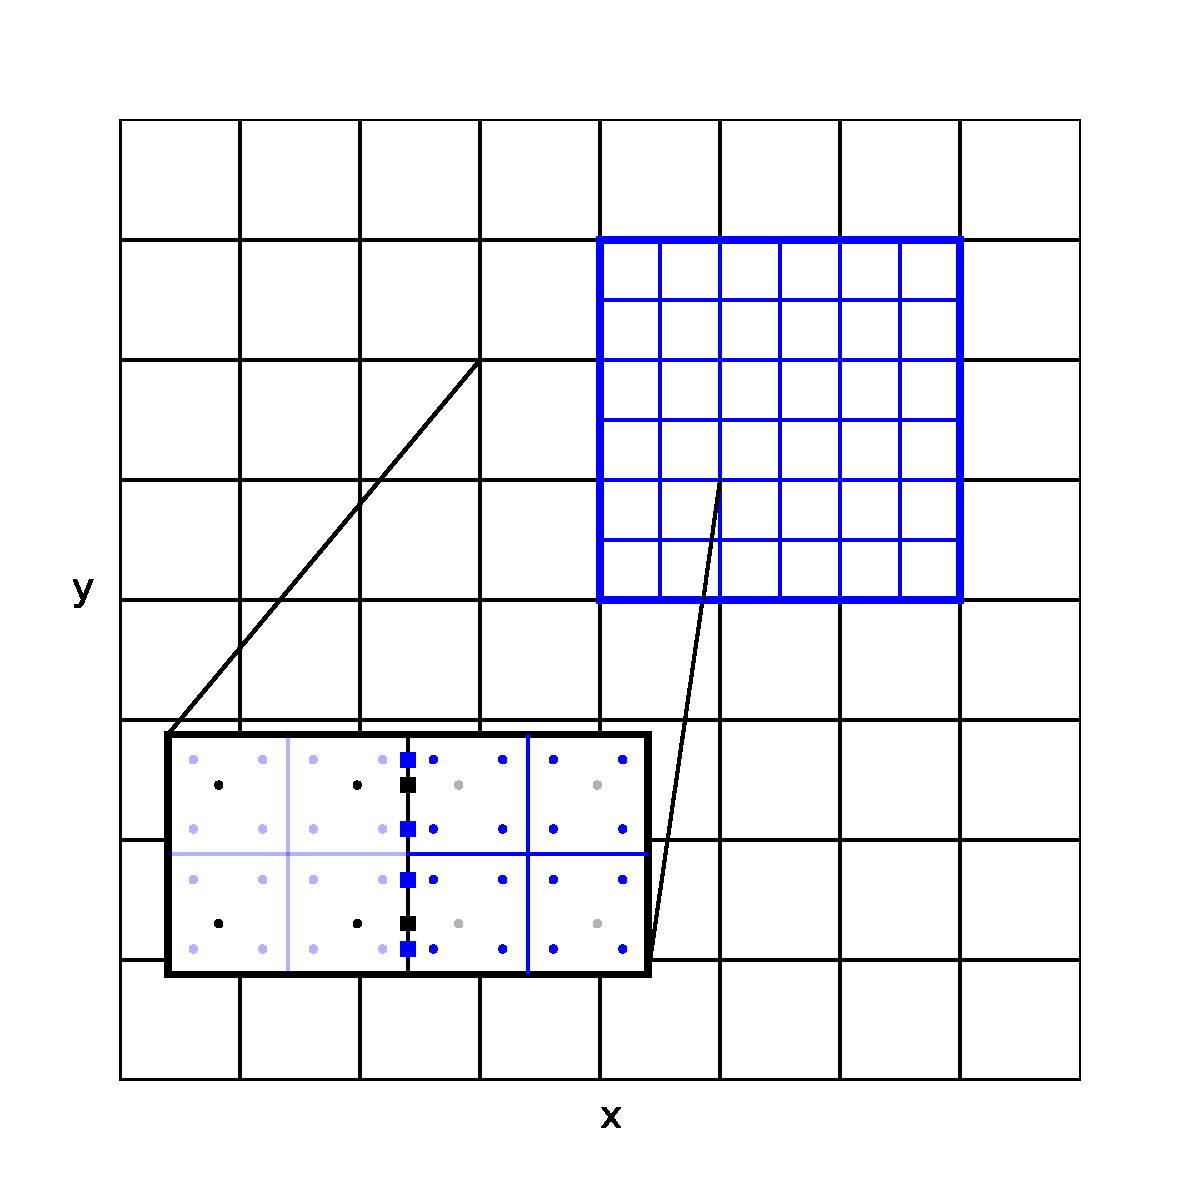
\includegraphics[width=0.5\textwidth]{fig.MeshRefinement_2D.pdf}
  \caption{Cartoon depicting a 2D mesh with two levels of refinement
  for a second-order DG method.
  The black lines mark the mesh element interfaces on the coarser level
  and the blue lines mark those on the finer level.
  The black dots denote the Legendre--Gauss quadrature points on the coarser
  level and the blue dots denote those on the finer level.
  The solid black squares denote the Legendre--Gauss quadrature points
  on the interface between two elements on the coarser level and the solid blue
  squares denote those between two elements on the finer level.
  The dots and lines with a degree of transparency should be viewed as
  belonging to ghost cells.
  }
  \label{fig.MR2D}
\end{figure}

%------------------------------------------------------------------------------%
\section{Results}

Here we present and discuss results from a suite of test problems designed to
test different aspects and capabilities of our solver.

\subsection{Sine Wave Advection}

Our first test problem examines the effects of the flux corrections on the
accuracy of our numerical method.
We investigate this with the one-dimensional linear advection of a
smooth density profile using an ideal \eos\ with $\Gamma=4/3$
and periodic boundary conditions.
At $t=0$ the density, velocity, and pressure are set to
\begin{equation}
  \rho\left(x\right)=1+0.1\,\sin\left(2\pi x/L\right),
  \hspace{1em}v\left(x\right)=0.1,\hspace{1em}p\left(x\right)=1,
\end{equation}
with $x\in\left[0,L\right]$ and $t\in\left[0,L/v\right]$, with $L=1$.
For these simulations, we apply neither the slope limiter nor the
bound-enforcing limiter.
By allowing the profile to advect until it returns to its original state,
we can quantify the accuracy of our method via, e.g., the relative error of
the density, $E_{1}\left[\rho_{h}\right]$, which we define as
\begin{equation}
  E_{1}\left[\rho_{h}\right]
  :=\frac{\int_{\mc{D}}\left|\rho_{h}\left(L/v,x\right)
          -\rho\left(x\right)\right|\,dx}
         {\int_{\mc{D}}\left|\rho\left(x\right)\right|\,dx}.
  \label{eq.Error}
\end{equation}
The integrals in \myeqref{eq.Error} are computed with Gaussian quadrature,
using ten quadrature points per element.
In order to assess the effect of the flux corrections, we perform eight
simulations: four with a single-level mesh, two with a two-level mesh
where flux corrections are not applied,
and two with a two-level mesh where flux corrections are applied.
For the two-level mesh simulations, we place the (stationary)
refinement boundary at $L/2$.
Each simulation has $N=\NSSPRK$.
Our results are shown in \tabref{tab.CR}.
% Generated by /home/kkadoogan/Work/Analysis/thornadoHydroXCFC_MethodsPaper_Software/./computeL1Error.py
% on 2024-02-03 17:43:15.562823
% Modified to work with Vanderbilt dissertation format
\begin{table}[b]
  \scriptsize
  \renewcommand{\tabcolsep}{0.09cm}
  \centering
  \begin{tabularx}{0.4\textwidth}{cccccc} \\
    \toprule \\
    $N$              &
    $\NK$            &
    Mesh             &
    Flux Corrections &
    $E_{\rho}$       \\ \\
    \midrule \\
2 & 32 & Single & N/A & $2.19\times10^{-5}$ \\
2 & 48 & Multi & Yes & $1.20\times10^{-5}$ \\
2 & 48 & Multi & No & $3.59\times10^{-4}$ \\
2 & 64 & Single & N/A & $5.13\times10^{-6}$ \\
3 & 32 & Single & N/A & $7.00\times10^{-6}$ \\
3 & 48 & Multi & Yes & $3.07\times10^{-6}$ \\
3 & 48 & Multi & No & $1.42\times10^{-5}$ \\
3 & 64 & Single & N/A & $9.77\times10^{-7}$ \\
  \bottomrule \\
  \end{tabularx}
  \caption{%
Effects of flux corrections on the accuracy
of our numerical method.
The first column is the number of DG nodes per element,
the second column is the number of elements,
the third column specifies whether or not the simulation used a single-
or multi-level mesh,
the fourth column specifies whether or not a multi-level mesh simulation
applied flux corrections,
and the fifth column denotes the error as defined in
\myeqref{eq.Error}.}
  \label{tab.CR}
\end{table}


The first point we note is that, for a given number of DG nodes and
a single-level mesh, the error decreases with increasing
resolution, as expected.
The second point we note that is that, defining $\NK$ as the number of
elements, when going from, e.g., $\NK=32$ with a single-level mesh
to $\NK=48$ with a two-level mesh and not applying flux corrections,
the error increases;
however, when going from $\NK=32$ with a single-level mesh
to $\NK=48$ with a two-level mesh and applying flux corrections,
the error decreases.
This demonstrates the importance of the flux corrections in this simple
scenario;
this effect is enhanced in more complicated flows.

\subsection{Sod's Shock Tube}

Our next test problem is the well-known (to those who know it well)
Sod shock tube \citep{s1978},
with open boundary conditions,
$\Gamma=4/3$,
$t\in\left[0,0.4\right]$,
$x\in\left[0,1\right]$ with the discontinuity situated at $x=0.5$,
and the left and right states of the fluid at $t=0$ given by
\begin{alignat*}{3}
  &\rho_{\textsc{l}}=1,\hspace{1em}
  &v_{\textsc{l}}=0,\hspace{1em}
  &p_{\textsc{l}}=1 \\
  &\rho_{\textsc{r}}=0.125,\hspace{1em}
  &v_{\textsc{r}}=0,\hspace{1em}
  &p_{\textsc{r}}=0.1.
\end{alignat*}
We refine the mesh based on the gradient of the density in order to capture
the shock and the contact discontinuity.
We obtain the exact solution for this problem with the code presented
in \citet{mm2003}.
Our results are shown in \figref{fig.Sod}.
The single-level mesh simulation ($\NK=256$) captures all discontinuities well.
The AMR simulation, which has $\NK=16$ on its coarsest level and $\NK=256$
on its finest level, captures the discontinuities as well as the single-level
mesh simulation and uses fewer degrees of freedom in the smooth regions; e.g.,
outside of the Riemann fan and in the post-shock and post-contact flow regions.
\begin{figure}[htb!]
  \centering
  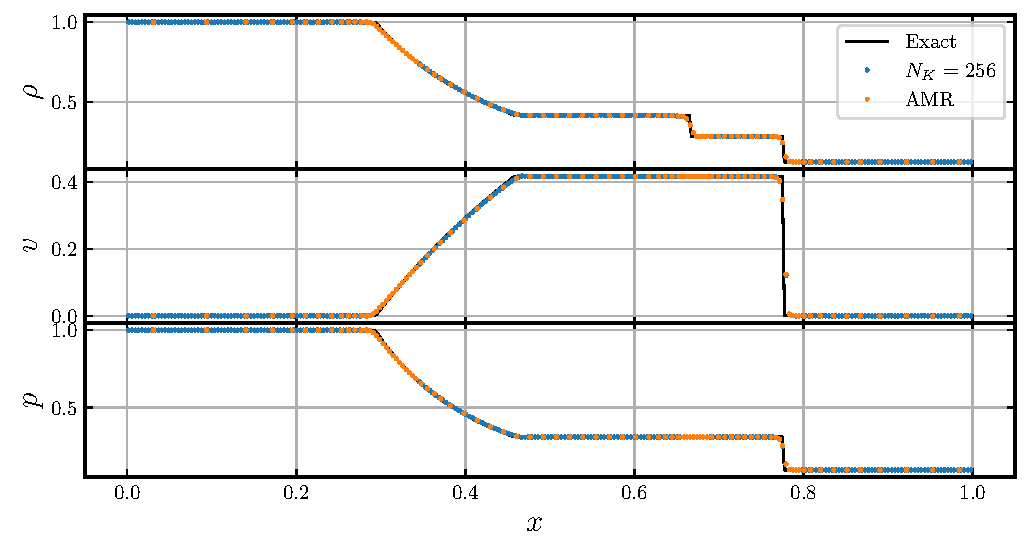
\includegraphics[width=0.9\textwidth]{fig.Sod.pdf}
  \caption{
Comoving baryon mass density (top panel),
velocity (middle panel),
and pressure (bottom panel),
plotted as functions of space at $t=0.4$ for the Sod shock tube problem.
Numerical results are shown as dots and
analytical results are shown as solid lines.
Single-level mesh results with $\NK=256$ are shown in blue
and five-level mesh results are shown in orange.}
  \label{fig.Sod}
\end{figure}

\subsection{2D Blast Wave}

Our next test is a 2D blast wave from \citet{db2002},
which tests the code's
ability to resolve strong shocks in multiple dimensions.
The setup for the problem is
$\Gamma=5/3$,
$t\in\left[0,0.4\right]$,
$x\times y\in\left[0,1\right]\times\left[0,1\right]$
with discontinuities located at $x=0.5$ and $y=0.5$,
open boundary conditions,
and the state of the fluid at $t=0$ given by
\begin{align}
\begin{split}
  \left(\rho_{\textsc{ne}},v^{1}_{\textsc{ne}},
  v^{2}_{\textsc{ne}},p_{\textsc{ne}}\right)
  &=\left(0.1,0,0,0.01\right) \\
  \left(\rho_{\textsc{nw}},v^{1}_{\textsc{nw}},
  v^{2}_{\textsc{nw}},p_{\textsc{nw}}\right)
  &=\left(0.1,0.99,0,1\right) \\
  \left(\rho_{\textsc{sw}},v^{1}_{\textsc{sw}},
  v^{2}_{\textsc{sw}},p_{\textsc{sw}}\right)
  &=\left(0.5,0,0,1\right) \\
  \left(\rho_{\textsc{se}},v^{1}_{\textsc{se}},
  v^{2}_{\textsc{se}},p_{\textsc{se}}\right)
  &=\left(0.1,0,0.99,1\right)
\end{split},
\end{align}
where the subscripts refer to the four quadrants of the domain
(north-east, north-west, south-west, south-east).
We perform two simulations: one using a single-level mesh and $256^{2}$
elements and another using a four-level mesh with $32^{2}$
elements on the coarsest level
and, therefore, $256^{2}$ elements on the finest level.
Both simulations have $N=3$ and $\NSSPRK=3$.
For the four-level mesh run, the tagging criteria are based
on the gradient of the density.
Our results are shown in \figref{fig.dZB2002}.
In the single-level mesh results (left panel),
the bow shock is well resolved.
The four-level mesh simulation (middle panel)
captures the shock with high resolution but, as can be seen in the right panel,
in regions outside the shock, the mesh is coarser, leading to a savings in
computation, walltime, and the size of the plotfiles.
Specifically, at the snapshot shown, the four-level mesh simulation has
21,736 leaf elements, while the single-level mesh simulation as 65,536
leaf elements.
There are features near
$x=0.6$, $y=0.6$, $x=0.2$, and $y=0.2$ that are clearly
visible in the single-level
mesh simulation, but are much fainter in the four-level mesh simulation.
This could likely be improved with an improved tagging criteria.
The same is true of the features near $x=0.85$ and $y=0.85$,
which are more diffusive in the four-level simulation
than they are in that of the single-level mesh.
\begin{figure}[htb!]
  \includegraphics[width=0.3\textwidth]%
    {fig.dZB2002_256x256.pdf}\hfill%
  \includegraphics[width=0.3\textwidth]%
    {fig.dZB2002_032x032_AMR.pdf}\hfill%
  \includegraphics[width=0.3\textwidth]%
    {fig.dZB2002_032x032_AMR_Mesh.pdf}
  \caption{Plots of the 2D blast wave from \citet{db2002}.
The left panel shows the pressure from
a single-level mesh simulation with $256^{2}$ elements,
the middle panel shows the pressure from a four-level mesh
simulation with $32^{2}$ elements on the coarsest level,
and the right panel shows the density from the same four-level
mesh simulation, and also overplots the mesh.}
  \label{fig.dZB2002}
\end{figure}

\subsection{Scaling Studies}

In addition to offering tools for mesh refinement, coupling to \amrex\
allows \thornado\ to run in parallel with MPI.
Because CCSN simulations are very computationally expensive,
any code aiming to simulate them must efficiently use all available
resources.
We present our results for both strong and weak scaling below.
All scaling results are shown for a "Bergamo" node on the ISAAC-NG
cluster at the University of Tennessee, Knoxville.

\subsubsection{Strong-scaling}

Strong-scaling allows a code to solve a problem with a fixed size quicker when
more processes are used.
To examine the strong-scaling capability of \thornado, we run
a problem having $256 \times 512=131,072$ elements with
1, 2, 4, 8, 16, 32, 64, and 128 MPI processes.
Our results are shown in \figref{fig.SS}.
We see ideal scaling out to $\sim\mc{O}\left(10^{6}\right)$ degrees of freedom
per process, and then good, but less than ideal scaling after that.
(This is likely due to the cost of communication between MPI processes
dominating over the cost of computation on a patch of data.)
We use this number to inform our weak-scaling study, which is described next.
\begin{figure}[htb!]
  \centering
  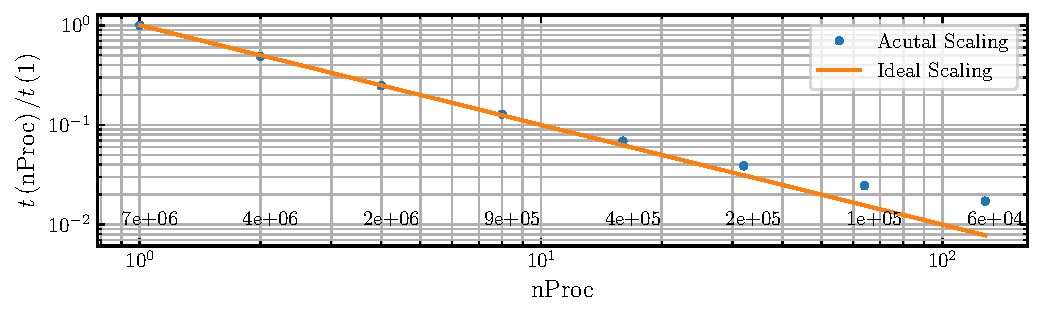
\includegraphics[width=0.8\textwidth]{fig.StrongScaling.pdf}
  \caption{The walltime to complete a simulation with different numbers of
processes, normalized to the walltime to complete the same simulation with one
process, plotted as a function of the number of processes.
Our data are shown as blue dots and the ideal scaling rate is shown as an
orange line.
The numbers reflect the approximate number of degrees of freedom per MPI
process for each simulation.}
  \label{fig.SS}
\end{figure}

\subsubsection{Weak-scaling}

Weak-scaling allows a code to run larger problems that would otherwise
overwhelm the memory of a single processor.
To examine the weak-scaling capability of \thornado, we keep the number
of degrees of freedom per process fixed and increase the problem
size.
Given that we see ideal strong-scaling out to $\mc{O}\left(10^{6}\right)$
degrees of freedom per MPI process, we use that value for our single-process
weak-scaling reference.
Our results are shown in \figref{fig.WS}.
We see reasonable weak-scaling out to 32 MPI processes.
\begin{figure}[htb!]
  \centering
  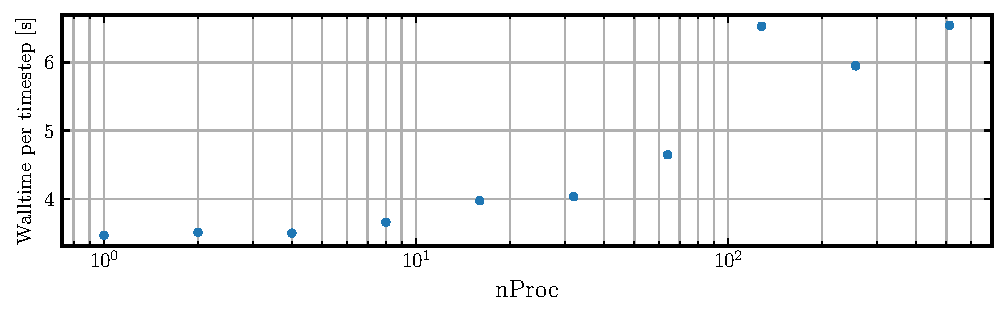
\includegraphics[width=0.8\textwidth]{fig.WeakScaling.pdf}
  \caption{The walltime per timestep in seconds vs.
the number of MPI processes.}
  \label{fig.WS}
\end{figure}

%------------------------------------------------------------------------------%
\section{Applications}

\subsection{1D Adiabatic Collapse}

Our second application is the 1D evolution of a 15 Solar mass progenitor
from \citet{wh2007} through collapse, bounce, and post-bounce phases with the
SFHo \eos, including self-gravity.
We first compare a single-level mesh simulation with resolution of 0.5 km
to a five-level mesh simulation with resolution on the finest level of 0.5 km.
Our refinement scheme is based on the density: at each new decade, starting
from $\rho=10^{9}\,\g\,\cm^{-3}$, a new level is added.

\subsubsection{Validation of AMR Implementation}

Our results from the collapse phase are shown in \figref{fig.Collapse_0.5km}.
We see that, overall, the two simulations agree.
There are slight differences as the system becomes
more compact; i.e., the five-level mesh simultation seems to be evolving
slightly quicker, as can be seen by the dashed lines moving slightly ahead
of the solid lines.
This may be an artifact of the two simulations not writing plotfiles at
exactly the same times.
\begin{figure}[htb!]
  \centering
  \includegraphics[width=0.8\textwidth]%
    {fig.AdiabaticCollapse_Collapse_dr0.50km.pdf}
  \caption{%
Mass density in grams per cubic centimeter (top left),
fluid velocity normalized to the speed of light (top right),
conformal factor (top of bottom left),
lapse function (bottom of bottom left),
and temperature in Kelvin (bottom right),
plotted as functions of radius in kilometers for a single-level mesh
simulation (solid) and for a five-level mesh simulation (dashed).
Each line corresponds to the density reaching a new decade.}
  \label{fig.Collapse_0.5km}
\end{figure}

Next, we discuss the post-bounce phase, the results from which are shown in
\figref{fig.PostBounce_0.5km}.
We again see general agreement with the single-level and five-level mesh
simulations.
We note differences in the post-shock entropy per baryon,
in particular, the oscillations in the flow are larger in the five-level mesh
simulation than in the single-level mesh simulation.
We attribute this to the coarser mesh in that region.
A tagging criteria that also accounts for the bounce shock may mitigate
this issue.
\begin{figure}[htb!]
  \centering
  \includegraphics[width=0.8\textwidth]%
    {fig.AdiabaticCollapse_PostBounce_dr0.50km.pdf}
  \caption{%
Mass density in grams per cubic centimeter (top left),
temperature in Kelvin (top right),
electron fraction (bottom left),
and entropy per baryon in units of Boltzmann's constant (bottom right),
plotted as functions of radius in kilometers
for the same simulations as are shown in
\figref{fig.Collapse_0.5km}.
The snapshots are chosen such that the shock radius, $\rsh$, is,
for each simulation,
$\rsh/\left(10^{3}\,\km\right)=\left(0.1,0.5,1,2,4,7.5\right)$.}
  \label{fig.PostBounce_0.5km}
\end{figure}

\subsection{Resolution Study}

\begin{figure}[htb!]
  \centering
  \includegraphics[width=0.8\textwidth]%
    {fig.CentralValues.pdf}
  \caption{Change in central entropy per baryon (top) and central
electron fraction (bottom) relative to their values at the beginning of
the simulations, plotted vs. central density in grams per cubic centimeter
(left) and vs. post-bounce time in milliseconds (right).
All runs use AMR and have 512 elements on the coarsest level.
The blue line corresponds to a seven-level run,
the orange line to a six-level run,
and the green line to a five-level run.
The vertical axis for the electron fraction plots has been scaled by $10^{5}$
in order to make the behavior of the the variables more clear.}
  \label{fig.CentralValues}
\end{figure}

\begin{figure}[htb!]
  \centering
  \includegraphics[width=0.8\textwidth]%
  {fig.CentralDensityVersusPostBounceTime.pdf}
  \caption{Central density in grams per cubic centimeter
vs. post-bounce time in milliseconds, offset by $0.6\,\ms$.
The lines corresponds to the same simulations as those in
\figref{fig.CentralValues}.}
  \label{fig.CentralDensity}
\end{figure}

%------------------------------------------------------------------------------%
\section{Software}

\href{https://amrex-codes.github.io/}{AMReX}
\citep{zab2019},
\href{https://matplotlib.org/}{Matplotlib}
\citep{h2007},
\href{http://www.numpy.org/}{NumPy}
\citep{hmw2020},
\href{https://yt-project.org/}{yt}
\citep{tso2011}

\section{Vector Components}

A generic four-vector, $u$, can be expanded in any coordinate basis
(e.g., the 3+1 coordinate basis),
$\left\{\p/\p x^{\mu}\right\}$, as
\begin{equation}
  u=u_{\left(x\right)}^{\mu}\,\pd{}{x^{\mu}},
\end{equation}
where $\p/\p x^{\mu}$ is the $\mu$-th basis vector
and $u_{\left(x\right)}^{\mu}$ is the $\mu$-th component of $u$ in
that basis.
In general, these basis vectors are not orthonormal;
i.e., $g\left(\p/\p x^{\mu},\p/\p x^{\nu}\right)
=:g^{\left(x\right)}_{\mu\nu}\neq\eta_{\mu\nu}$,
where, here, $g$ is the $\left(0,2\right)$ metric tensor.
We can also expand $u$ in an orthonormal basis, $\left\{e_{\mu}\right\}$,
\begin{equation}
  u=u^{\mu}\,e_{\mu},
\end{equation}
where the $e_{\mu}$ are defined such that
$g\left(e_{\mu},e_{\nu}\right)=\eta_{\mu\nu}$.
If $e_{0}$ is a four-velocity then this basis can be associated
with an observer, and $\left\{e_{\mu}\right\}$ can properly
be called a frame of reference.
In particular, if $e_{0}\equiv n$ (see \secref{ss.3+1}) then this frame defines
an Eulerian observer, and $\left\{e_{\mu}\right\}$ is the frame of
reference of an Eulerian observer.

As an example of immediate relevance,
the four-velocity of the fluid as measured by an Eulerian observer
in the 3+1 basis (in which the 0-th component is zero) is
\begin{equation}
  v=v_{\left(x\right)}^{\mu}\,\pd{}{x^{\mu}}
  =v_{\left(x\right)}^{i}\,\pd{}{x^{i}}.
\end{equation}
The $v_{\left(x\right)}^{i}$
are what we initialize in our test problems and applications.
In spherical-polar coordinates, this vector takes the form
\begin{equation}
  v=v_{\left(x\right)}^{r}\,\pd{}{r}
  +v_{\left(x\right)}^{\theta}\,\pd{}{\theta}
  +v_{\left(x\right)}^{\varphi}\,\pd{}{\varphi}.
\end{equation}
This should be contrasted with the perhaps more familiar form,
\begin{equation}
  v=v^{i}\,e_{i}
  =v^{r}\,e_{r}+v^{\theta}\,e_{\theta}
  +v^{\varphi}\,e_{\varphi},
\end{equation}
where
\begin{equation}
  e_{i}:=\left|\left|\pd{}{x^{i}}\right|\right|^{-1}\,
  \pd{}{x^{i}}\hspace{1em}\left(\mathrm{no\ sum\ over\ }i\right),
\end{equation}
with
\begin{equation}
  \left|\left|\pd{}{x^{i}}\right|\right|
  :=\left|g\left(\pd{}{x^{i}},
  \pd{}{x^{i}}\right)\right|^{1/2}
  =\left|g^{\left(x\right)}_{ii}\right|^{1/2}=h^{\left(x\right)}_{i},
\end{equation}
and where $h^{\left(x\right)}_{i}$ is the $i$-th scale factor in the
coordinate system $\left\{\p/\p x^{\mu}\right\}$.
From this, we see that the components of $v$ in the 3+1 basis,
$v_{\left(x\right)}^{i}$,
are related to the components of $v$ in the basis of the Eulerian
observer, $v^{i}$, as
\begin{equation}
  v^{i}
  =h^{\left(x\right)}_{i}\,v_{\left(x\right)}^{i}
  \ \left(\mathrm{no\ sum\ over\ }i\right).
\end{equation}

Also, note that the $v_{\left(x\right)}^{i}$ are different from
the coordinate velocities,
which are instead defined as (dropping the $\left(x\right)$ subscript)
\begin{equation}
  \dot{x}^{i}:=\td{x^{i}}{t}
  =\td{\tau}{t}\,\td{x^{i}}{\tau}
  =\frac{u^{i}}{u^{0}}
  =\frac{W}{u^{0}}\left(v^{i}+n^{i}\right)
  =\alpha\left(v^{i}+n^{i}\right)
  =\alpha\,v^{i}-\beta^{i}.
\end{equation}


%------------------------------------------------------------------------------%

\chapter{Summary, Conclusions, and Outlook}
\label{ch.con}

We have shown, via detailed numerical simulations, that GR may play an
important role in our further understanding of the SASI, and that for simulation codes to
accurately predict observables, they should use GR gravity and GR hydrodynamics.
In particular, in order to correctly capture the growth rate of the
instability, GR must be used.
This is important for the creation of templates for gravitational waves
and may also be important for CCSNe with more massive progenitors.
As mentioned in the conclusion of Chapter~\ref{ch.sasi},
next steps for this project include performing 3D simulations.
The behavior of the additional spiral modes may also influenced by GR,
and only simulations will reveal that.
The simulations we have performed revealed aspects of the pure SASI and its
behavior under GR;
it would also be worthwhile to perform simulations with some implementation of
neutrino transport because the SASI in CCSNe may behave differently than
the SASI we have investigated.
This would be difficult because disentangling neutrino-driven convection
from the SASI would be a non-trivial task.

We have detailed our implementation of the DG method to solve the GRHD
``Euler--Einstein" system of equations.
This includes how we mitigate spurious oscillations,
enforce physical bounds, and update the solution in time.
Additionally, we discussed how we coupled \thornado\ to \poseidon,
a gravity solver for the \xcfc\ system of equations.
We have also detailed our coupling to \amrex, including how we interpolate
fluid fields across different levels of refinement in a conservative manner
and how we achieve conservation across coarse-to-fine interfaces.
We have checked our implementation by performing several
simulations of test-problems as well as by simulating the adiabatic collapse,
bounce, and
post-bounce evolution of a 15 Solar mass progenitor in parallel, with AMR.
Future work includes performing the same simulation but in 2D and 3D.
This will take some development because of the restriction on the timestep
imposed at the origin and at the poles;
one possible remedy is to implement a filtering scheme as is done in
\texttt{SphericalNR} \citep{jmz2023}.
Future work also includes
simulating a SASI as we have done in \citet{dem2023}, but using AMR.
We will compute the power in the $\ell=1$ mode for simulations performed
with and without AMR and examine the results.
Future work will also involve comparing the AMR adiabatic collapse simulations
to determine what resolution is sufficient to maintain stability of the PNS.

Beyond finishing the methods paper, future work involves porting the
\thornado-\amrex\ coupling to GPUs,
a necessity for taking full advantage of current, and future,
leadership-class supercomputers.
Future work also includes coupling the existing framework to the DG, GR
neutrino transport module and performing full, three-dimensional
CCSN simulations.
This will bring its own challenges, particularly in multi-dimensional simulations
because of the large number of degrees of freedom imposed by a spectral,
multi-group two-moment scheme.

In the meantime, we have a code that solves the GRHD equations in AMR coupled
to an \xcfc\ metric solver.
This code is free and open-source and available to anyone who wishes to use it
for their application.
For example, the code could potentially be used to simulate the late stages
of a CCSN progenitor, when the neutrinos are all in the free-streaming regime.


\singlespacing
%\bibliographystyle{apalike}
\bibliographystyle{aasjournal}
\bibliography{main}{}


\end{document}
